\documentclass[]{course-notes}

\title{Design \& Make}
\author[Gopsill \& Valentine]{\normalsize James Gopsill \& Rod Valentine}

\begin{document}

\maketitle

\begin{abstract}
    The Design \& Make exercise introduces Engineering Design Process Models, Principles of Design \& Manufacture, and Project Management techniques. 
    The lectures provides a overview of the techniques that are typically employed whilst the exercise provides an opportunity to put some of these techniques into practice as you design a product to meet a design brief. 
    You will then manufacture and assemble your design in the 2nd year. This document contains the course notes that support the exercise and lectures.
\end{abstract}

\clearpage
\setcounter{tocdepth}{2}
\tableofcontents

\clearpage
\listoffigures

\clearpage
\listoftables

\clearpage
\section*{List of Acronyms}
\begin{acronym}[TDMA]
    \acro{BOM}{Bill of Materials}
    \acro{CAD}{Computer Aided Design}
    \acro{CNC}{Computer Numerically Controlled}
    \acro{CPM}{Critical Path Methods}
    \acro{DfA}{Design for Assembly}
    \acro{DfM}{Design for Manufacture}
    \acro{DfX}{Design for X}
    \acro{DMLS}{Direct Metal Laser Sintering}
    \acro{FDM}{Fused Deposition Modelling}
    \acro{FFF}{Fused Filament Fabrication}
    \acro{MCDA}{Multi-Criteria Decision Analysis}
    \acro{NASA}{National Aeronautics and Space Administration}
    \acro{PDS}{Product Design Specification}
    \acro{PERT}{Project Evaluation and Review Techniques}
    \acro{PLM}{Product Lifecycle Management}
    \acro{SLM}{Selective Laser Melting}
    \acro{SLS}{Selective Laser Sintering}
    \acro{STL}{Stereolithography}
    \acro{VDI2221}{Systematic Design Process Model}
\end{acronym}

\section{Introduction}

\newthought{The aim of this exercise}\marginnote{intended learning outcomes} is to introduce you to Engineering Design Process Models, Principles of Design \& Manufacture, and Project Management techniques. 
The lectures provides a overview of the techniques that are typically employed whilst the exercise provides an opportunity to put some of these techniques into practice as you design a product to meet a design brief, which you will then manufacture in your 2nd year.

Over the next five weeks you will be introduced to:

\begin{itemize}
  \item Defining Engineering Design;
  \item Design Process Models;
  \item The Design Brief and Product Design Specification;
  \item Concept Design;
  \item Concept Selection;
  \item Design for X;
  \item Rapid Prototyping; and,
  \item Project Management Essentials.
\end{itemize}

To\marginnote{support} support the exercise, there are lectures and tutorial classes that you should attend. 
In addition, there is a Moodle course page containing support material and a Q\&A forum. 
All out of lecture and tutorial hour queries should be submitted to the Q\&A. 
This enables us to provide fair and balanced feedback across the all the groups.

As the coursework builds on the previous weeks work, it is crucial that you keep up-to-date to avoid overloading yourselves at the end. These exercises have been developed so that you can begin to experience and learn how best to manage your team and the tasks that need to be completed.

\cref{tbl-lectures} provides an overview of the lecture and pre-work that should be performed ahead of the tutorial session so you can ask for feedback in the sessions.

\begin{table}[h!]
    \caption{Supporting lecture and tutorial sessions}
    \label{tbl-lectures}
    \centering
    \small
    \begin{tabular}{r p{0.4\textwidth} p{0.4\textwidth}}
        \toprule
        
        Week & Lecture & Activities \\
        
        \midrule

        07 & 
        Exercise, Design Process Models \& Product Design Specification & 
        PDS \& Morphological Chart \\
        
        08 & 
        Concept Generation \& Concept Selection 
        & Concept Selection \\
        
        09 & 
        Embodiment Design \& Design for Assembly & 
        Embodiment Design \& Design for Assembly \\
        
        10 & 
        Design for Manufacture & 
        Design for Manufacture \\
        
        11 & 
        Project Management Essentials & 
        Design Report \\

    \bottomrule
    \end{tabular}
\end{table}

As with your Engineering Drawing classes\marginnote{feedback}, you will be given formative feedback throughout your tutorials. These are supported by staff and post-graduate researchers. This is your opportunity to get feedback on your design work, so use this time wisely. You are expected to work outside of these hours and that you come to the tutorial sessions ready with questions concerning your design.

Engineering Design\marginnote{significance of engineering design} is the discipline of transferring your theoretical knowledge and understanding of engineering systems into practical and usable products. You may find it interesting to discover that up to 80\% of the committed cost of a product occurs when decisions are made early-on in its design \pref{fig-committed}.\cite{ullman2002}\cite{corbett1986}\cite{mileham1993}

\begin{figure}[t!]
    \centering
    \includestandalone[width=0.9\textwidth]{01_introduction/commited-cost}
    \caption[The committed cost during a design project]{The committed cost during a design project~\citep{ullman2002}}
  \label{fig-committed}
\end{figure}

It is the objective of the designer to consider all the potential implications of these decisions and their impact across the Product's Lifecycle. This is becoming evermore critical as companies become more reliant on the sale of products as part of a service, which is often referred to as Product Service Systems. For example, Rolls-Royce's sale strategy is now focused on the idea of `Power by the Hour'. Thus, issues in the design of the product can greatly impact the profitability and safety of the service they provide.

With companies becoming ever-more global, engineering teams are often collaborating across the world on new product development. The competencies and skills that you will develop throughout your design exercises in Bath will enable you to meet these challenges head-on.

It\marginnote{thirty-three percent} may also be interesting to know that the majority of you will progress into higher-levels of management, be it in an engineering, consultancy, medical, banking, start-up and/or other industrial sectors. The success of engineers in business is further demonstrated by the fact that a third of the top Chief Executive Officers (CEO's) have an engineering degree.\cite{bi2011}\cite{hbr2014} Nearly as many who have an MBA! 

\section{Defining Engineering Design}

\newthought{Over the years}, there has been many attempts to define Engineering Design. 
This has been a non-trivial task and is mainly due to the increasingly complex and multi-disciplinary nature of design. 
An element that continue to increase over the years with the rate of technological development.

\marginnote{fielden report}In the first two years of the Bath Engineering Degree, we will be focusing on the design of mechanical components, systems and machines. 
Therefore, we will be using Fielden's definition of Engineering Design:

\begin{center}
  ``The use of scientific principles, technical information and imagination in the definition of a mechanical structure, machine or system to perform pre-specified function with the maximum economy and efficiency.''~\cite{fielden1963}
\end{center}

\citeauthor{pahl2013}~\cite{pahl2013} also provides an interesting perspective on Engineering Design and how it forms the bridge between the sciences (\cref{fig-ed}). It is being able to analyse and critique designs both objectively and subjectively, which is key to being a Design Engineer.

\begin{figure*}
    \centering
    \includestandalone[width=0.75\textwidth, mode=buildnew]{02_engineering_design/cross-over}
    \caption[Positioning Engineering Design within the sciences]{Positioning Engineering Design within the sciences~\citep{pahl2013}}\label{fig-ed}
\end{figure*}

\section{Design Process Models}

Design process models exist at the core of any engineering design exercise. They aid us in defining the approach and the key stages we will take to develop a solution to a given problem. Now, there are a large number of approaches that researchers and industry have developed over the years. \citeauthor{wynn2017}\cite{wynn2017} recent review of process models in design and development revealed that there are over 50 different models, which range from mapping the entire product development process to supporting specific elements of the process. These models also take different perspectives to how Engineering Design should be managed such as abstract, analytical, management science and procedural. 

\begin{figure*}[h!]
  \centering
  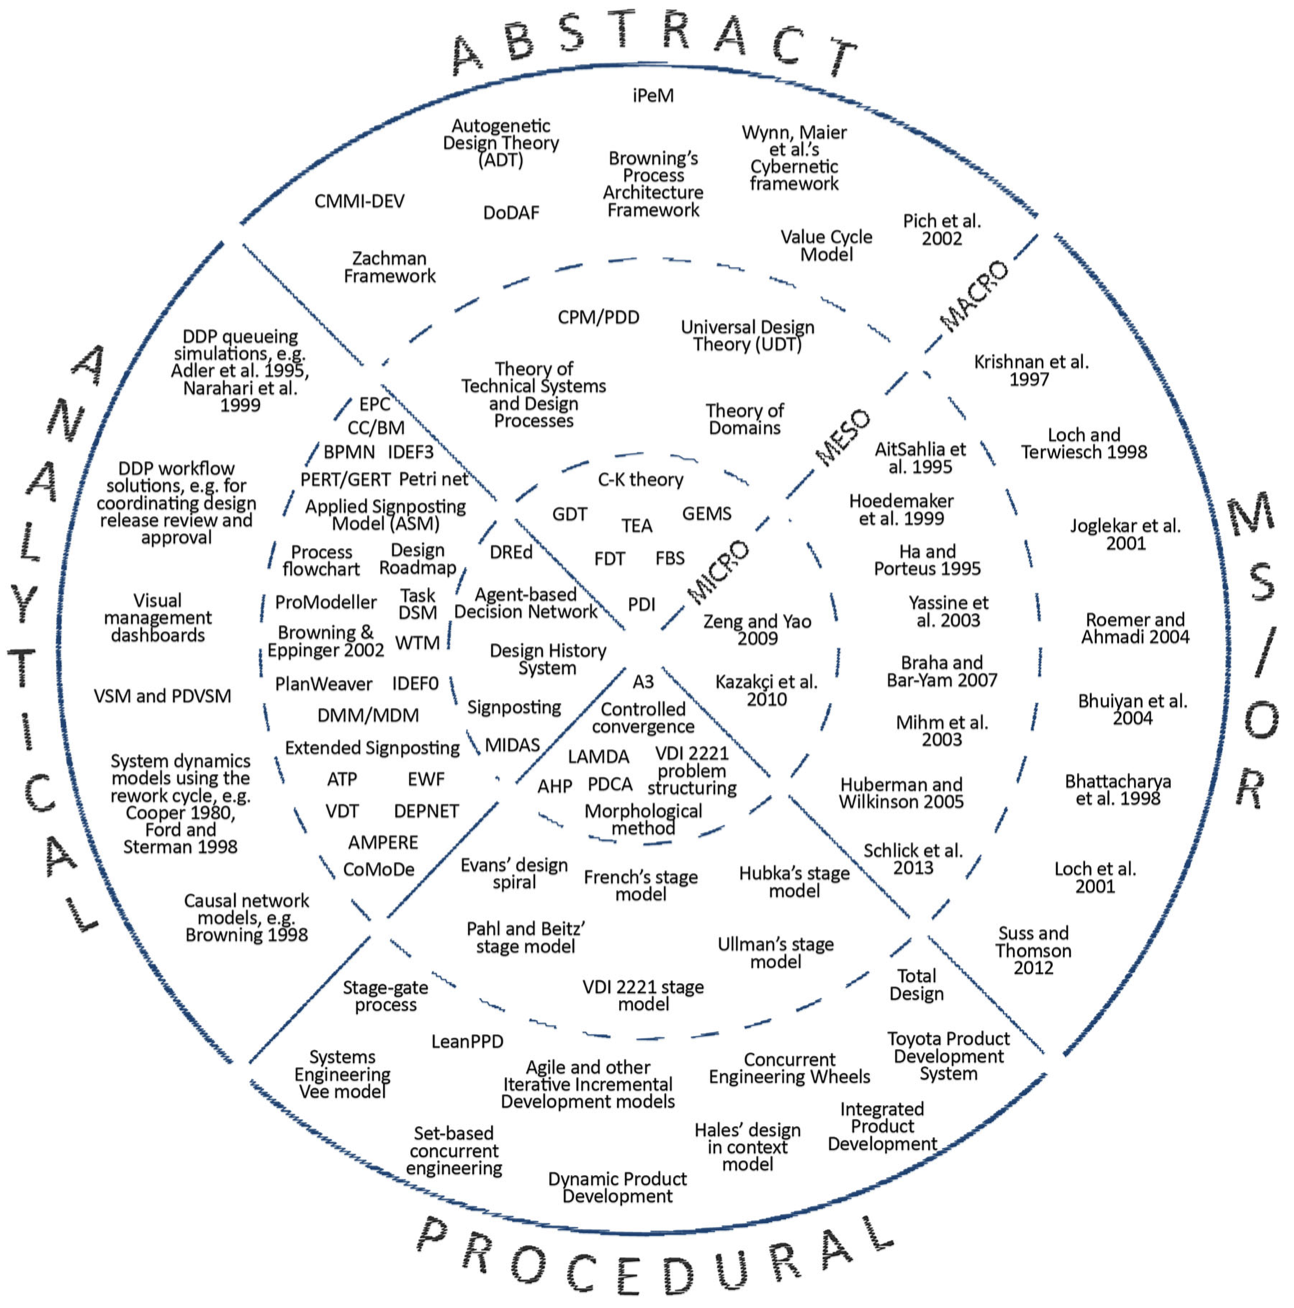
\includegraphics[width=0.8\textwidth]{03_design_process_models/wynn-review.png}
  \caption[Mapping of design process models against their scope and type]{Mapping of design process models against their scope and type~\citep{wynn2017}}
\end{figure*}


It is often the case that industry will customise a generic approach to fit their culture and domain. Many companies, particularly engineering consultancies, have identified that it is not only the solution but the process they take to solve problems that provides them with a competitive advantage in business. 

In this section, we will cover four commonly adopted models:

\begin{enumerate}
  %\item The Systematic Design Process VDI2221
  \item VDI2221 -- Systematic Design Process Model
  \item V-Model
  \item Design Double Diamond
  \item Stage-Gate Model
\end{enumerate}


\subsection{VDI2221 -- Systematic Design Process Model}

The \acf{VDI2221} was developed by senior designers from industry and academia. The aim was to provide a generic approach for the design of products within the fields of mechanical, precision, control, software and process engineering. The approach (\cref{fig-vdi}) includes seven basic working steps.

As this process was designed for general applicability, the \ac{VDI2221} has a very abstract structure, thus permitting product-specific and company-specific variations. \cref{fig-vdi} should therefore be regarded as a guideline to which detailed working procedures can be assigned. Special emphasis is placed on the iterative nature of the approach and the sequence of the steps must not be considered rigid. Some steps might be omitted, and others repeated frequently. This flexibility is in accordance with practical design experience and enables companies to frame their processes in a similar manner to enable communication of where they are in their product development cycle.

\begin{figure*}[h!]
    \centering
    \includestandalone[width=0.6\textwidth, mode=buildnew]{03_design_process_models/VDI2221}
    \caption[Systematic Design Approach]{Systematic Design Approach~\citep{pahl2013}}\label{fig-vdi}
\end{figure*}



\subsection{Design Double Diamond}

The Design Council\cite{council2007} illustrates the design process as a Double Diamond (\cref{fig-dd}), which is divided into four distinct phases:

\begin{enumerate}
    \item Discover
    \item Define
    \item Develop
    \item Deliver
\end{enumerate}

\begin{figure}[h!]
    \centering
    \includestandalone[width=0.7\textwidth, mode=buildnew]{03_design_process_models/double_diamond}
    \caption[Design Double Diamond]{Design Double Diamond}\label{fig-dd}
\end{figure}

In all creative processes a number of possible ideas are created (`divergent thinking') before refining and narrowing down to the best idea (`convergent thinking'), and this can be represented by a diamond shape. The Double Diamond indicates that this happens twice – once to confirm the problem definition and once to create the solution. One of the greatest mistakes is to omit the left-hand diamond and end up solving the wrong problem.

In order to discover which ideas are best, the creative process is iterative. This means that ideas are developed, tested and refined a number of times, with weak ideas dropped in the process. This cycle is an essential part of good design.

Practical design methods -- like user diaries, journey mapping and character profiles -- move a project through the four phases of the Double Diamond. 

The\marginnote{discover} first quarter of the Double Diamond model covers the start of the project. Designers try to look at the world in a fresh way, notice new things and gather insights.

The\marginnote{define} second quarter represents the definition stage, in which designers try to make sense of all the possibilities identified in the Discover phase. Which matters most? Which should we act on first? What is feasible? The goal here is to develop a clear creative brief that frames the fundamental design challenge.

The\marginnote{develop} third quarter marks a period of development where solutions or concepts are created, prototyped, tested and iterated. This process of trial and error helps designers to improve and refine their ideas.

The\marginnote{delivery} fourth and final quarter of the double diamond model is the delivery stage, where the resulting project (a product, service or environment, for example) is finalised, produced and launched.

\subsection{V-Model}

The V-Model \pref{fig-v-model} has been widely adopted across systems design where a product can be split into separate sub-systems that can be developed and tested independently from one another.
The left-hand side of the ``V'' details the processes that organisations follow to decompose the list of requirements for a product into a set of separate system element specifications that are then used to generate a set of designs for the sub-systems of the product.

The sub-systems can then be tested independently before being integrated until the full product is formed (right-hand side of the `V'). 
Testing is performed at each stage of the integration of the systems, which simplifies the identification of issues as the product is built-up.

\begin{figure*}[h!]
    \centering
    \includestandalone[width=0.8\textwidth]{03_design_process_models/v-model.tex}
    \caption{Systems Engineering V-Model}\label{fig-v-model}
\end{figure*}


\subsection{Stage/Phase-Gate Model}

Stage/Phase-Gate models arose during the management of large-scale projects for mechanical and chemical engineering in the 1940s. One of the major organisations to develop this model further was in the \acf{NASA}.
\ac{NASA} introduced its phased review process in the 1960s and broke up the development of their projects into a series of phases that could be individually reviewed.

\begin{figure*}
    \centering
    \includestandalone[width=0.9\textwidth]{03_design_process_models/stage-gate}
    \caption{Stage-Gate Model}\label{fig-stage}
\end{figure*}

The phased review process consisted of five stage with periodic development reviews between stages \pref{fig-stage}. 
The stages phases are:

\begin{table}
    \begin{tabular}{r l}
        Start & Discovery \& Idea Generation \\
        Stage 1 & Scoping \\
        Stage 2 & Building the Business Case \\
        Stage 3 & Development \\
        Stage 4 & Testing \& Validation \\
        Stage 5 & Launch \\
    \end{tabular}
\end{table}

The\marginnote{start} design team will be given a design brief that provides a high-level abstraction of a problem that they are trying to solve. From this, the organisation will begin to develop potential ideas that will solve this problem using concept generation techniques. 

These ideas will then be presented at the first gate review where they will follow a concept selection technique to decide which idea(s) will continue into the scoping stage of the project. It is not uncommon for more than one idea to continue into the next stage if budget and resource is available.

With\marginnote{stage one: scoping} the ideas selected, the project continues into Stage 1 of the model. This is where engineers evaluate the product and the market that it will be entering. Engineers need to consider the strengths and weaknesses of the product and what it is going to offer to the potential consumer. 

Analysis of the competition enables the organisation to estimate the level of market penetration the potential product might have. This information is then fed back into the review gate where the senior management team will decide whether to continue with the development of the product. Remember, this model is typically applied to large engineering projects that are potentially worth Millions or Billions of pounds. Thus, these organisations need to be clear of the business opportunity before committing their resources to a project.

If\marginnote{stage two: building the business case} a clear market gap and engineering solution has been presented, and the organisation has decided to go ahead, the engineers then move into Stage 2, which is to fully define and build the business case around the project. This is the last stage before the commitment of engineering work and resource is made to the project. Business cases and their format can vary considerably between industries but in general, they will include reports detailing the product definition, business case, project plan, and review of the projects' feasibility.

After\marginnote{stage three: development} review of the business case, the organisation will decide whether to continue on with the project. If accepted, the project moves into Stage 3, which is where the project is actually executed. This covers the product's design and development, and will include some early prototyping and stakeholder feedback.

The results of this stage is a fully-functional prototype of the product that is to be manufactured and sold. This will be taken into the review where it will be critiqued in relation to the PDS and further checking of the business case to ensure the opportunity in the market still exists.

With\marginnote{stage four: testing and validation} the prototype fully developed, the project can move into the testing and validation stage. This is where the prototype will be tested in a variety of use cases and provided to the stakeholders for trialling and feedback.

If\marginnote{stage five: launch} the testing and validation is successful, the organisation is now is ready to launch the product and ramp-up production.

\subsection{This Design Exercise}

In this exercise, we will be adapting \ac{VDI2221} and follow the process shown in \cref{fig-dm-process}.
The process has been developed to map with University timetabling and study hours for the course.

\begin{figure}[h!]
    \centering
    \includestandalone[width=0.65\textwidth]{03_design_process_models/design_and_make}
    \caption{Design \& Make Design Process}\label{fig-dm-process}
\end{figure}

The\marginnote{design brief} exercise will begin with a design brief and is the general problem that you're going to try and solve. In doing so, you will need to clarify elements of the task and start to build the boundaries and constraints in order to solve the design problem.

The\marginnote{product design specification} formalisation of these boundaries and constraints comes in the development of a \acf{PDS}. Your design will need to meet these requirements in order to be a valid solution to the problem. The PDS will be a mixture of subjective and objective requirements, which will be used to assess the viability of your design ideas. 

With\marginnote{concept generation} the requirements set, we will then move into the concept generation stage. This is where you will develop a number of concepts that will aim to meet the PDS. To develop these concepts, we will be discussing and applying some concept generation techniques. The aim of concept generation is to diverge by exploring the design space and developing as many potential ideas as possible. No matter how crazy they may seem!

Now\marginnote{concept selection} we have a number of potential concepts, we need to begin to converge by assessing the concepts against the \ac{PDS}. We will be introducing you to four techniques to do this.

\marginnote{embodiment design} Having selected the final concept, it is time to develop the concept further by refining how the components will interact and fix against one another. This is where engineers perform a comprehensive analysis of all the forces, heat transfer, fluid flow, system dynamics and/or kinematics relating to the product.

This provides us with a preliminary layout of all the components within the product and estimates for the component sizes.

This\marginnote{detail design} takes us into the detail design section of the design process and is where you will be selecting components, drawing up components for manufacture and developing the instructions for the assembly of the prototype. In this stage, you will be using the ideas from Design for Assembly and Design for Manufacture to further refine the design. The result will be the instructions of producing the parts, generating the purchase orders for the suppliers and creating a \acf{BOM} for the prototype.

\section{Product Design Specification}

\newthought{The \acf{PDS}} is a description of what you intend to design and lists all the requirements that a design needs to achieve in order to meet the customers needs. 
There are many ways a \ac{PDS} can be collated and formed, and in this exercise we will be using the format as shown in \cref{tbl-pds} and contains the following information:


\begin{table}
    \small
    \begin{tabular}{r p{0.6\textwidth}}
        No. & Requirement number or revision number. \\
        Date & Date captured. \\
        Source & Reference to the material used to generate the requirement. \\
        Requirement & A description of the requirement. \\
        Target & A quantitative or qualitative metric that should be attained by the design. \\
        Must/Wish & Whether the requirement must be achieved by the design or you wish the design to achieve it. \\ 
        Method of Evaluation & A description of how you have evaluated your design against this requirement (e.g.\ force/stress calculations, user survey and/or expert vote). \\
        Cross-reference & Position in the report that this requirement is discussed.
    \end{tabular}
\end{table}

\begin{table*}[h!]
    \centering
    \caption{Product Design Specification Template}
    \label{tbl-pds}
    \small
    \begin{tabular}{l l l l l l l l}
        \toprule
        No. & Date & Source & Requirement & Target & Must/Wish & Method of Evaluation & Cross-Ref \\
        \midrule
        1 & & & & \\
        Rev 1a & & & & \\
        2 & & & & \\
        \ldots & & & & \\
        \bottomrule
    \end{tabular}
    \vspace{1em}
\end{table*}

\marginnote[3em]{garvins' dimensions of quality} In addition to this, there are a variety of ways one can breakdown the \ac{PDS} to ensure that all aspects are covered. This could be by component/sub-system or looking at the design from a number of different perspective. One such breakdown is Garvins' Dimensions of Quality\cite{garvin1987}, which are defined as:

\begin{table}
    \small
    \begin{tabular}{r p{0.6\textwidth}}
        Performance & The operating characteristics of the design \\
        Features & Additional capabilities and characteristics of the design \\
        Reliability & Factors that effect the likelihood of failure of the design in a specific time period \\
        Conformance & The standards and rules to which a design must adhere (i.e.\ health and safety) \\
        Durability & Factors that affect the lifespan of the design \\
        Serviceability & Factors that affect the maintenance of the design \\
        Aesthetics & Factors relating to how the design looks \\
        Manufacture \& Assembly & Factors relating to how the design is made and assembled \\
    \end{tabular}
\end{table}

\section{Concept Generation}\label{sec-concept-generation}

\newthought{Concept generation is a fundamental part} of any Engineering Design process. In this section, we discuss four methods that can be used in generating concepts.

\begin{enumerate}
    \item Brainstorming
    \item Competitor analysis \& patent search
    \item Morphological charts
    \item Prototyping \& construction kits
\end{enumerate}

\subsection{Brainstorming}

Brainstorming is a technique by which a group attempts to find a solution for a specific problem by amassing all the members' ideas spontaneously. Although many consider brainstorming as an ad-hoc exercise where teams get together to form ideas, rules and guidelines to maximise the creative output have been developed.

\begin{marginfigure}
    \centering
    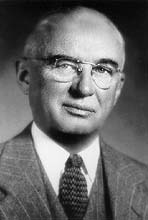
\includegraphics[width=0.7\textwidth]{05_concept_generation/osborn.jpg}
    \caption[Alex Osborn]{Alex Osborn}
    \label{fig-osborn}
\end{marginfigure}

Alex Osborn was one of the first to develop a rule-set for brainstorming. The objective was to improve the creation of new ideas within business meetings. 

The rules can be summarised as:

\begin{itemize}
  \item No criticism of ideas
  \item Go for large quantities of ideas
  \item Build on other ideas or combine them
  \item Encourage wild and unusual ideas
\end{itemize}

Through these rules, his studies revealed that more ideas were created and \emph{``quantity produced quality''}.

Since then, there have been many more studies into brainstorming and methods that can support the generation of ideas. Here are a just a few of them \pref{fig-brainstorm}.

\begin{figure}[h!]
    \centering
    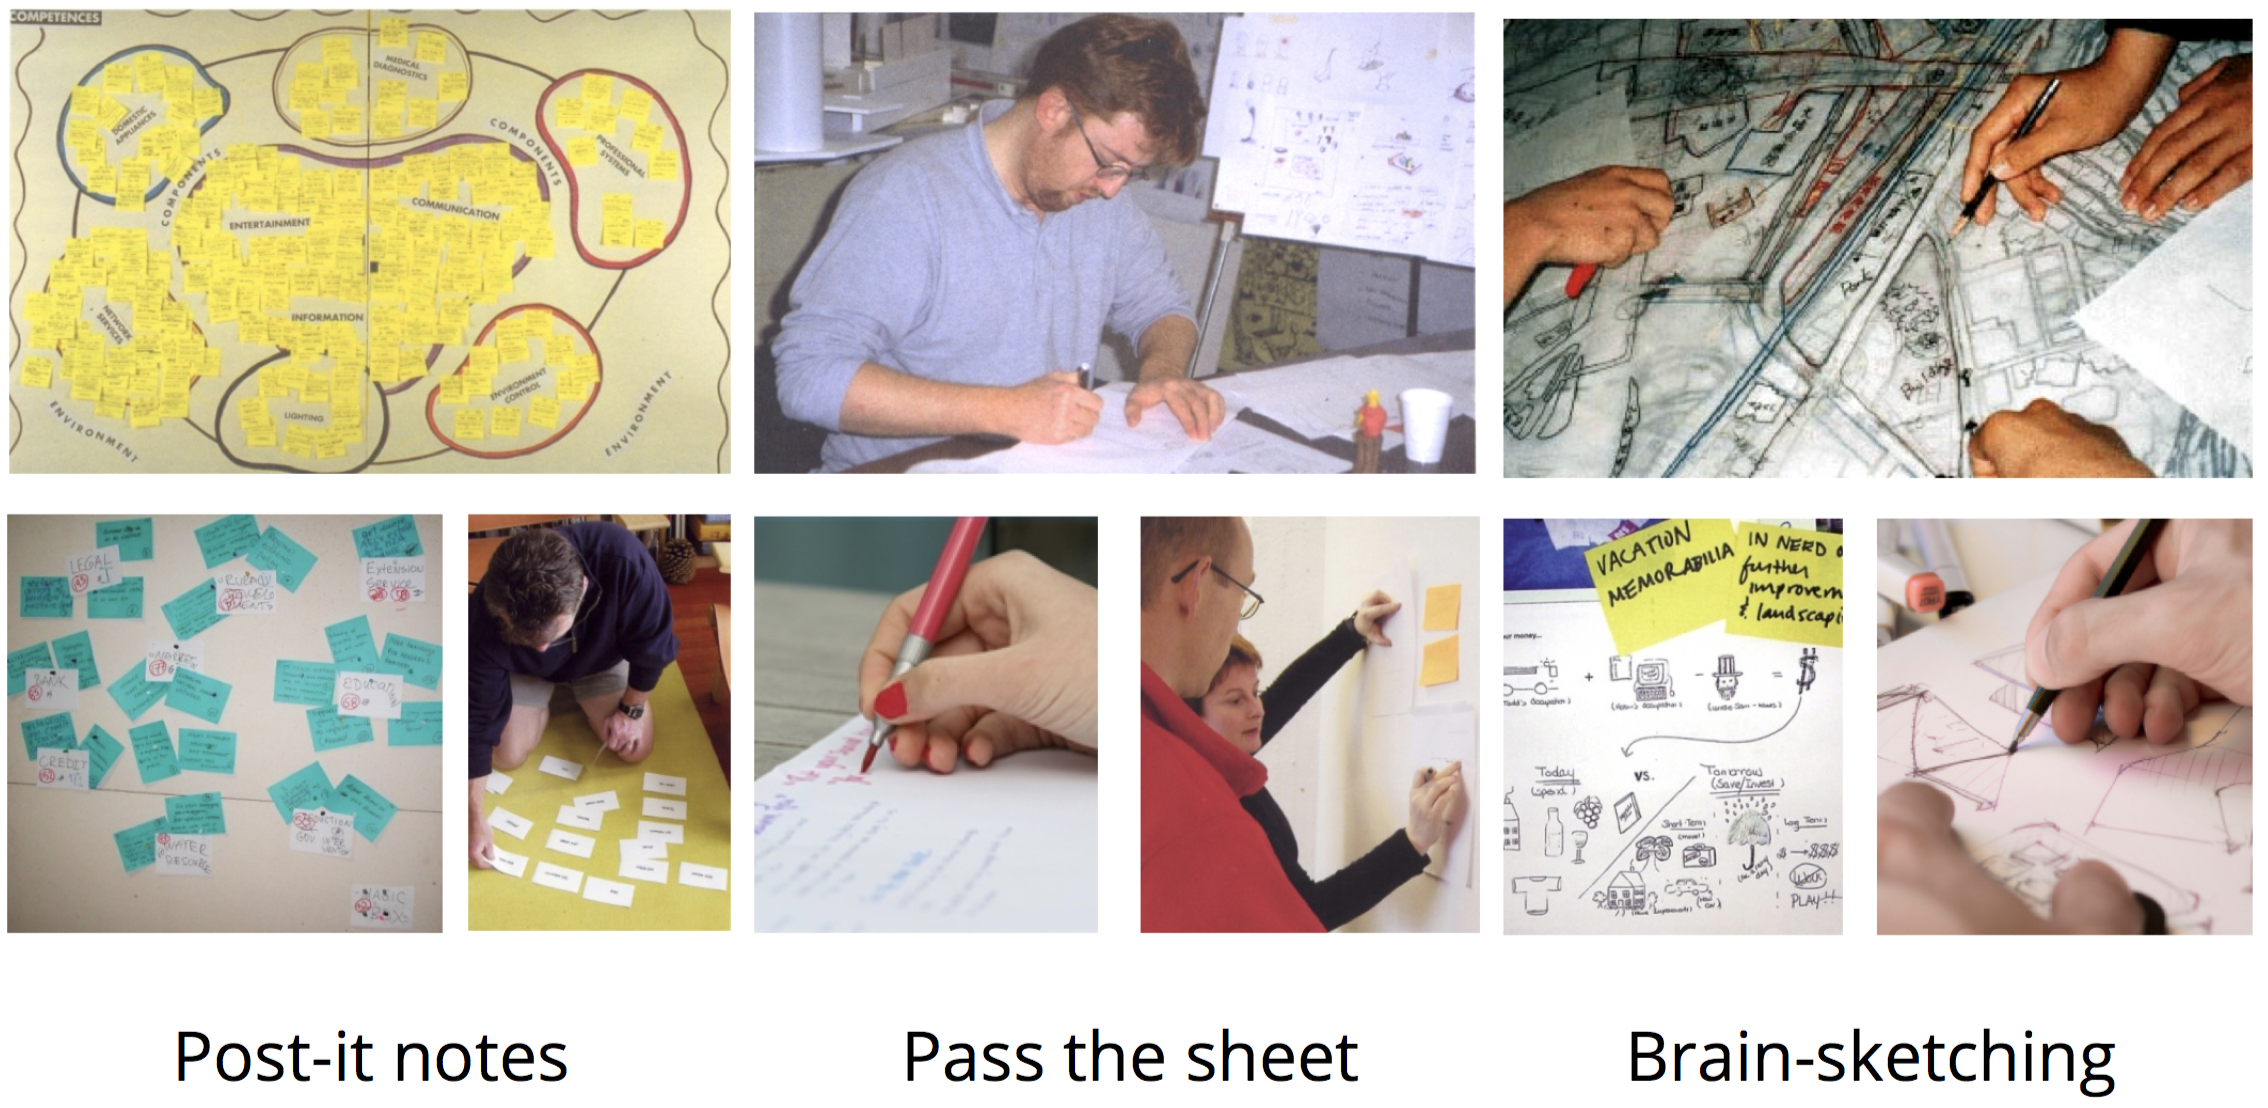
\includegraphics[width=0.95\textwidth]{05_concept_generation/brainstorm.png}
    \caption{Brainstorming techniques}
    \label{fig-brainstorm}
\end{figure}


The\marginnote{post-it notes} `Post-it Note' exercise requires engineers to write and/or sketch onto a post-it note. This is then placed on the table for the rest of the group to see. As more notes are added, the facilitator can start to form groups of notes that follow a similar theme and/or answer a particular part of the design task.

In\marginnote{pass the sheet} the `Pass the Sheet' exercise, each designer is given a sheet of paper and are asked to write a couple of sentences for a potential idea to solve the problem. These are then passed around to the next designer in the group who tries to build-upon the existing idea by writing an additional couple of sentences. Once passed around the whole group, the ideas are read aloud and a discussion is had on the relative merits from each one. The group then converges upon one of the ideas and/or combine features of each to develop their final concepts.

In\marginnote{brain-sketching} `Brain-sketching', the group is not aloud to talk or write their ideas. All they can do is sketch. Annotations on the sketches may be permitted to convey what the item is. This is a great way of tackling challenges where form and/or packaging is a critical issue. 

With\marginnote{running a session} one of these methods selected, the common approach to running a brainstorming session is as follows:

\begin{table}
    \small
    \begin{tabular}{r p{0.6\textwidth}}
        Assign a facilitator & It's their job to make sure everybody is contributing, keep everyone on track and record ideas. \\
        Record everything & Every idea that anyone says should be drawn or written down. \\
        Build on others & Use everyone else's ideas as a starting point for more of your own. \\
        Contribute & Everyone should speak or draw.  Take it turns if required. \\
        Park ideas & If you are struggling or hit a dead end, park that idea until later. \\
    \end{tabular}
\end{table}

\subsection{Competitor Analysis \& Patent Search}

More often than not, you will be developing a product that will be competing with and/or complementing an existing product line. Therefore, it is always a good idea to analyse existing products on the market with respect to your \ac{PDS}.  Patent searching also enables you to discover what attempts have been made to solve the problem and what aspects might be protected by people across the world.

The\marginnote{advantages} main advantages are that you will have confidence that a variation of an existing design has a greater potential to work when compared to a completely novel design. It also enables you to quickly generate potential designs. By comparing existing products to your PDS, you can start to identify areas that will make your product unique and help you decide where to focus your design resources and time on.

The\marginnote{disadvantages} potential issue in using existing products is that you have the potential to infringe on intellectual property and copyright.
The companies you will be working for will have legal teams to help you in deciding what elements of existing designs can be used.

\subsection{Morphological Charts}

Morphological charts are a great method for generating ideas where the product to be designed has clear functional and/or sub-system boundaries. For each function, designers can come up with a range of potential solutions.
From this, a matrix of function vs.\ solution can be created.
An example is shown in \cref{fig-morphological-chart}.


\begin{table*}[h!]
    \centering
    \caption[Morphological chart for a forklift truck]{Morphological chart for a forklift truck~\citep{cross1989}}
    \label{fig-morphological-chart}
    \small
    \begin{tabular}{l | c c c c c}
        \toprule
        Function & \multicolumn{5}{l}{Solution} \\
        \midrule
        Support & Wheels & Track & Air Cushion & Slides & Pedipulators \\
        Propulsion & Driven wheels & Air thrust & Moving cable & Linear induction \\
        Power & Electric & Petrol & Diesel & Bottled gas & Steam \\
        Transmission & Gears and shafts & Belts & Chains & Hydraulic & Flexible cable \\
        Steering & Turning wheels & Air thrust & Rails & & \\
        Stopping & Brakes & Reverse thrust & Ratchet & & \\
        Lifting & Hydraulic arm & Rack and pinion & Screw & Chain or rope hoist & \\
        Operator & Seated at front & Seated at rear & Standing & Walking & Remote control \\
        \bottomrule
    \end{tabular}
    \vspace{2em}
\end{table*}


Using this matrix, designers systematically analyse the potential combinations to provide an overall concept for a product.
This enables designers to generate a great number of concepts very quickly.
Theoretically, a \(10\times10\) matrix could yield \num{10e9} concepts for a product.


\subsection{Prototyping \& Construction Kits}

Prototyping \& construction kits are a great way of quickly refining and identifying potential geometric issues during the early design phases (\cref{fig-why-prototype}). The use of kits such as LEGO\texttrademark{} remove the potential bias introduced by the quality of designers' sketches and wording of ideas as all ideas are created to the same level of refinement. The simplicity of these kits also enables wider stakeholder engagement where you can have you customers and different departments involved in the generation of potential solutions. In some instances, the design problem can be very large with multiple dependencies between requirements. Prototyping is a method that can focus the designers attention to specific parts of the design problem, which can then be later combined to form an overall concept (\cref{fig-why-prototype}).

\begin{figure}[h!]
    \centering
    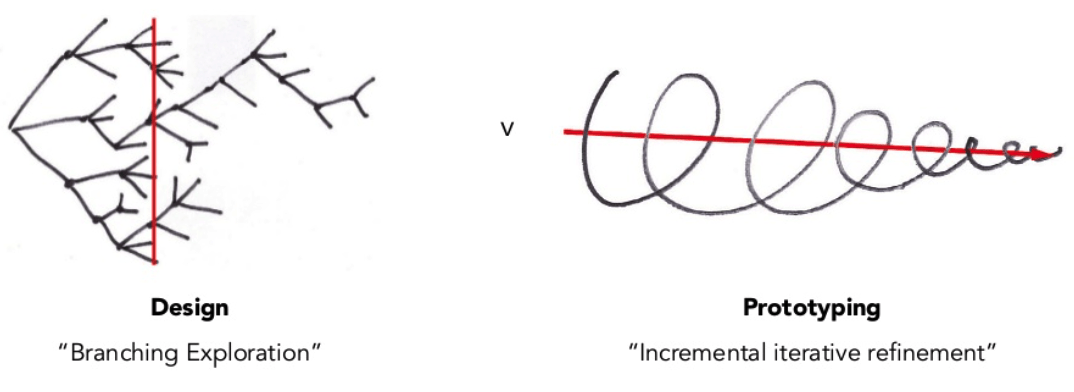
\includegraphics[width=0.9\textwidth]{05_concept_generation/whyprototype.png}
    \caption[Bill Buxton, Sketching User Experiences]{Bill Buxton, Sketching User Experiences~\citep{buxton2010}}
    \label{fig-why-prototype}
\end{figure}

However\marginnote{Research at Bath}, the use of prototyping and construction kits can introduce constraints and biases in the exploration of the solution space. 
For example, lets take 7 $2\times2$ LEGO\texttrademark{} bricks ($B_{2,2}(7)$), which we want to connect together by adding one brick at a time. In this scenario, there are \num{1.8e9} unique pathways of constructing the bricks and \num{1.3e6} morphologically unique combinations. The greater number of paths to unique combinations provide the perception that there are a lot more potential solutions than there actually are. Further, if one were to look at the number of pathways to each unique combination, some have more pathways than others and hence, are statistically more likely to be created by a designer. An example of this is shown in \cref{fig-combinations} and is part of the ongoing research at Bath where the findings are being used to help design future construction kits to support concept generation\cite{design2018}.

\begin{figure*}[ht!]

    %\hfill
    \subfloat[Combination 1\newline Number of Pathways: 8]{
        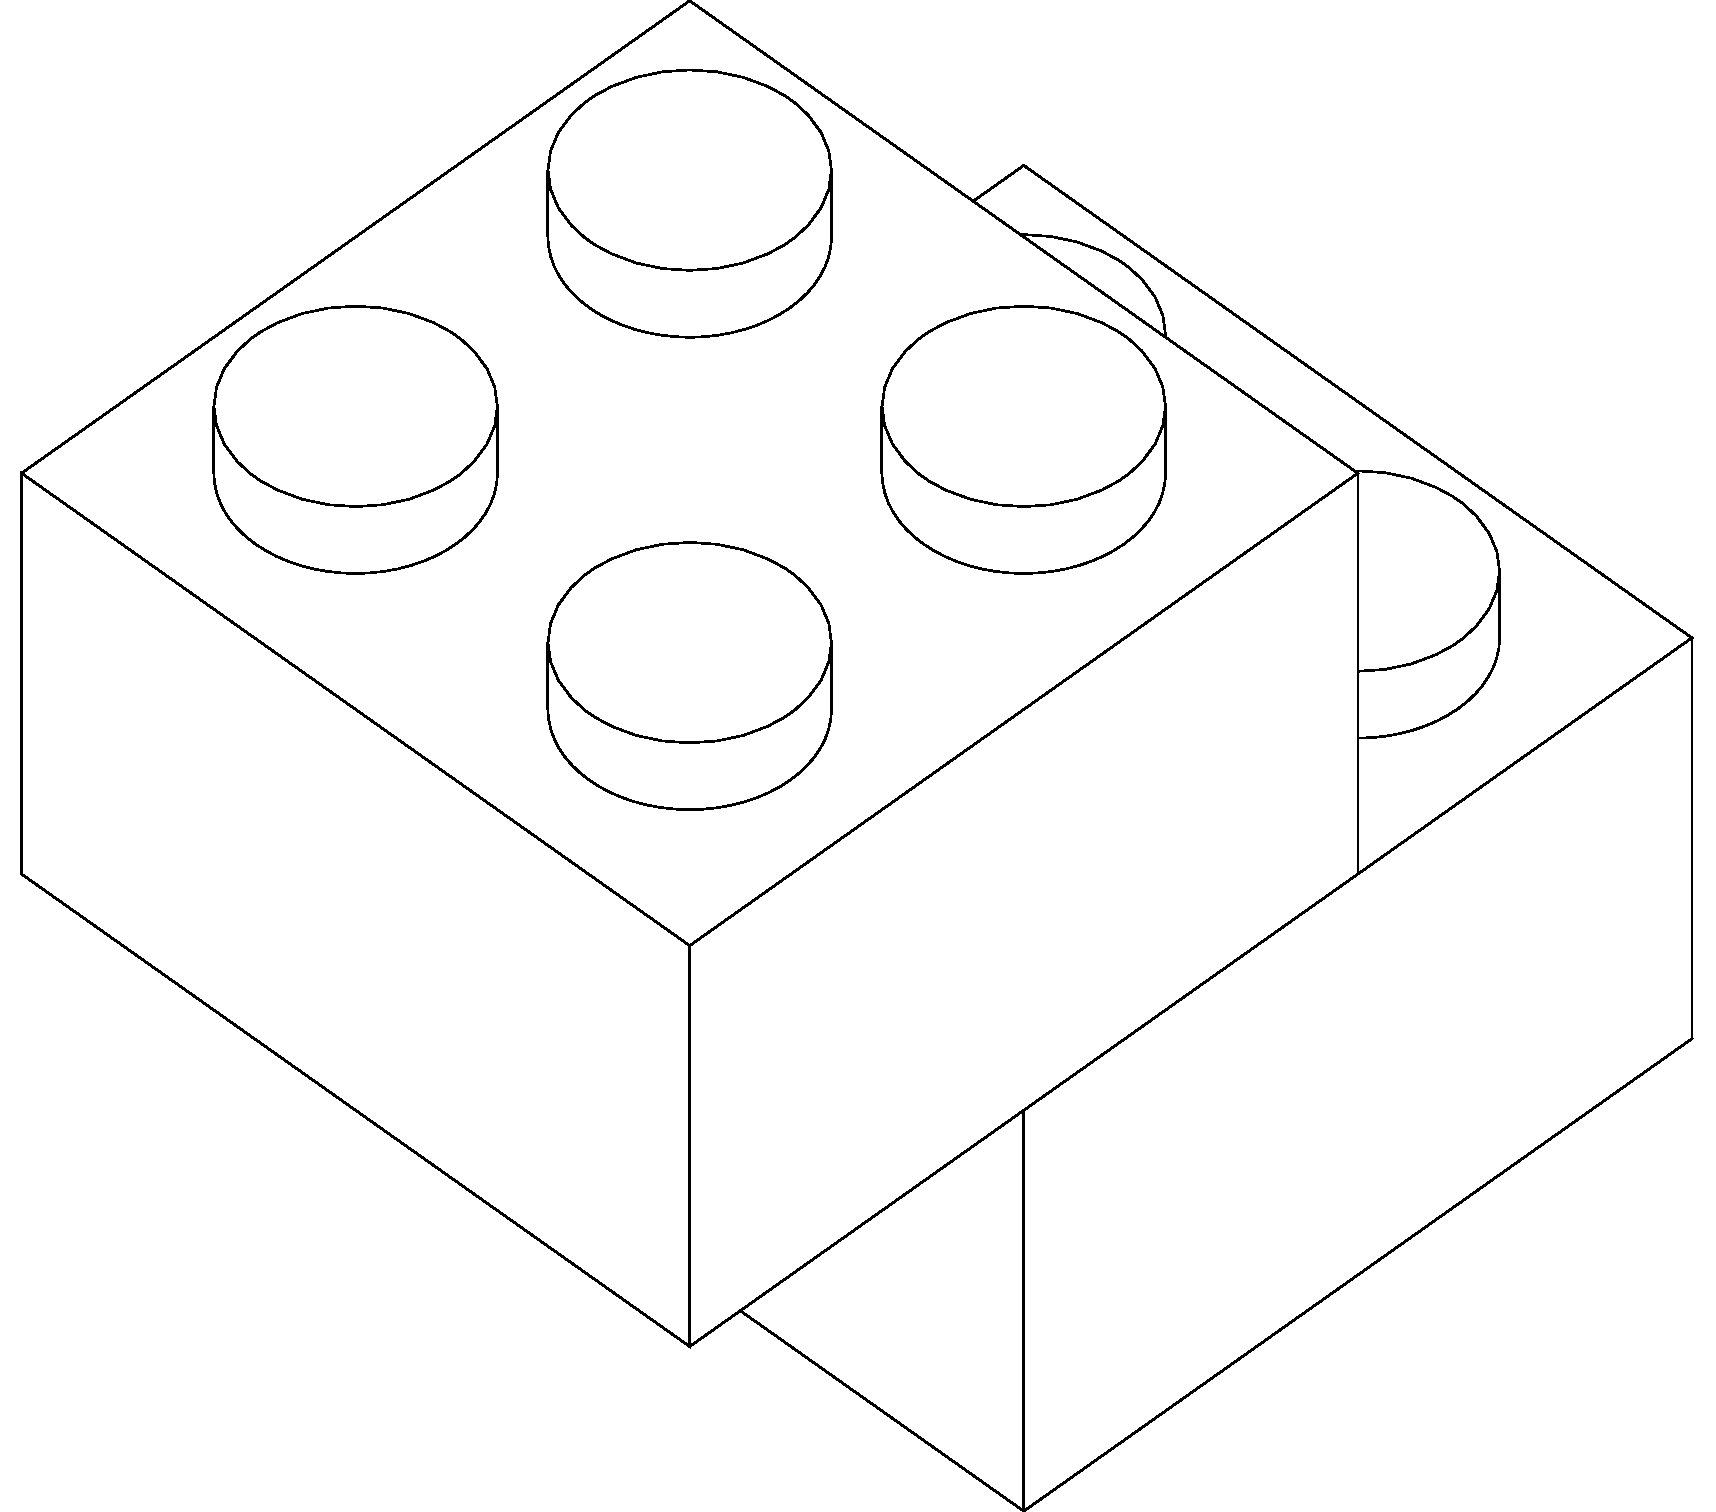
\includegraphics[height=4.5cm]{05_concept_generation/2x2-brick-combo-1.pdf}
    }
    \hfill
    \subfloat[Combination 2\newline Number of Pathways: 8]{
        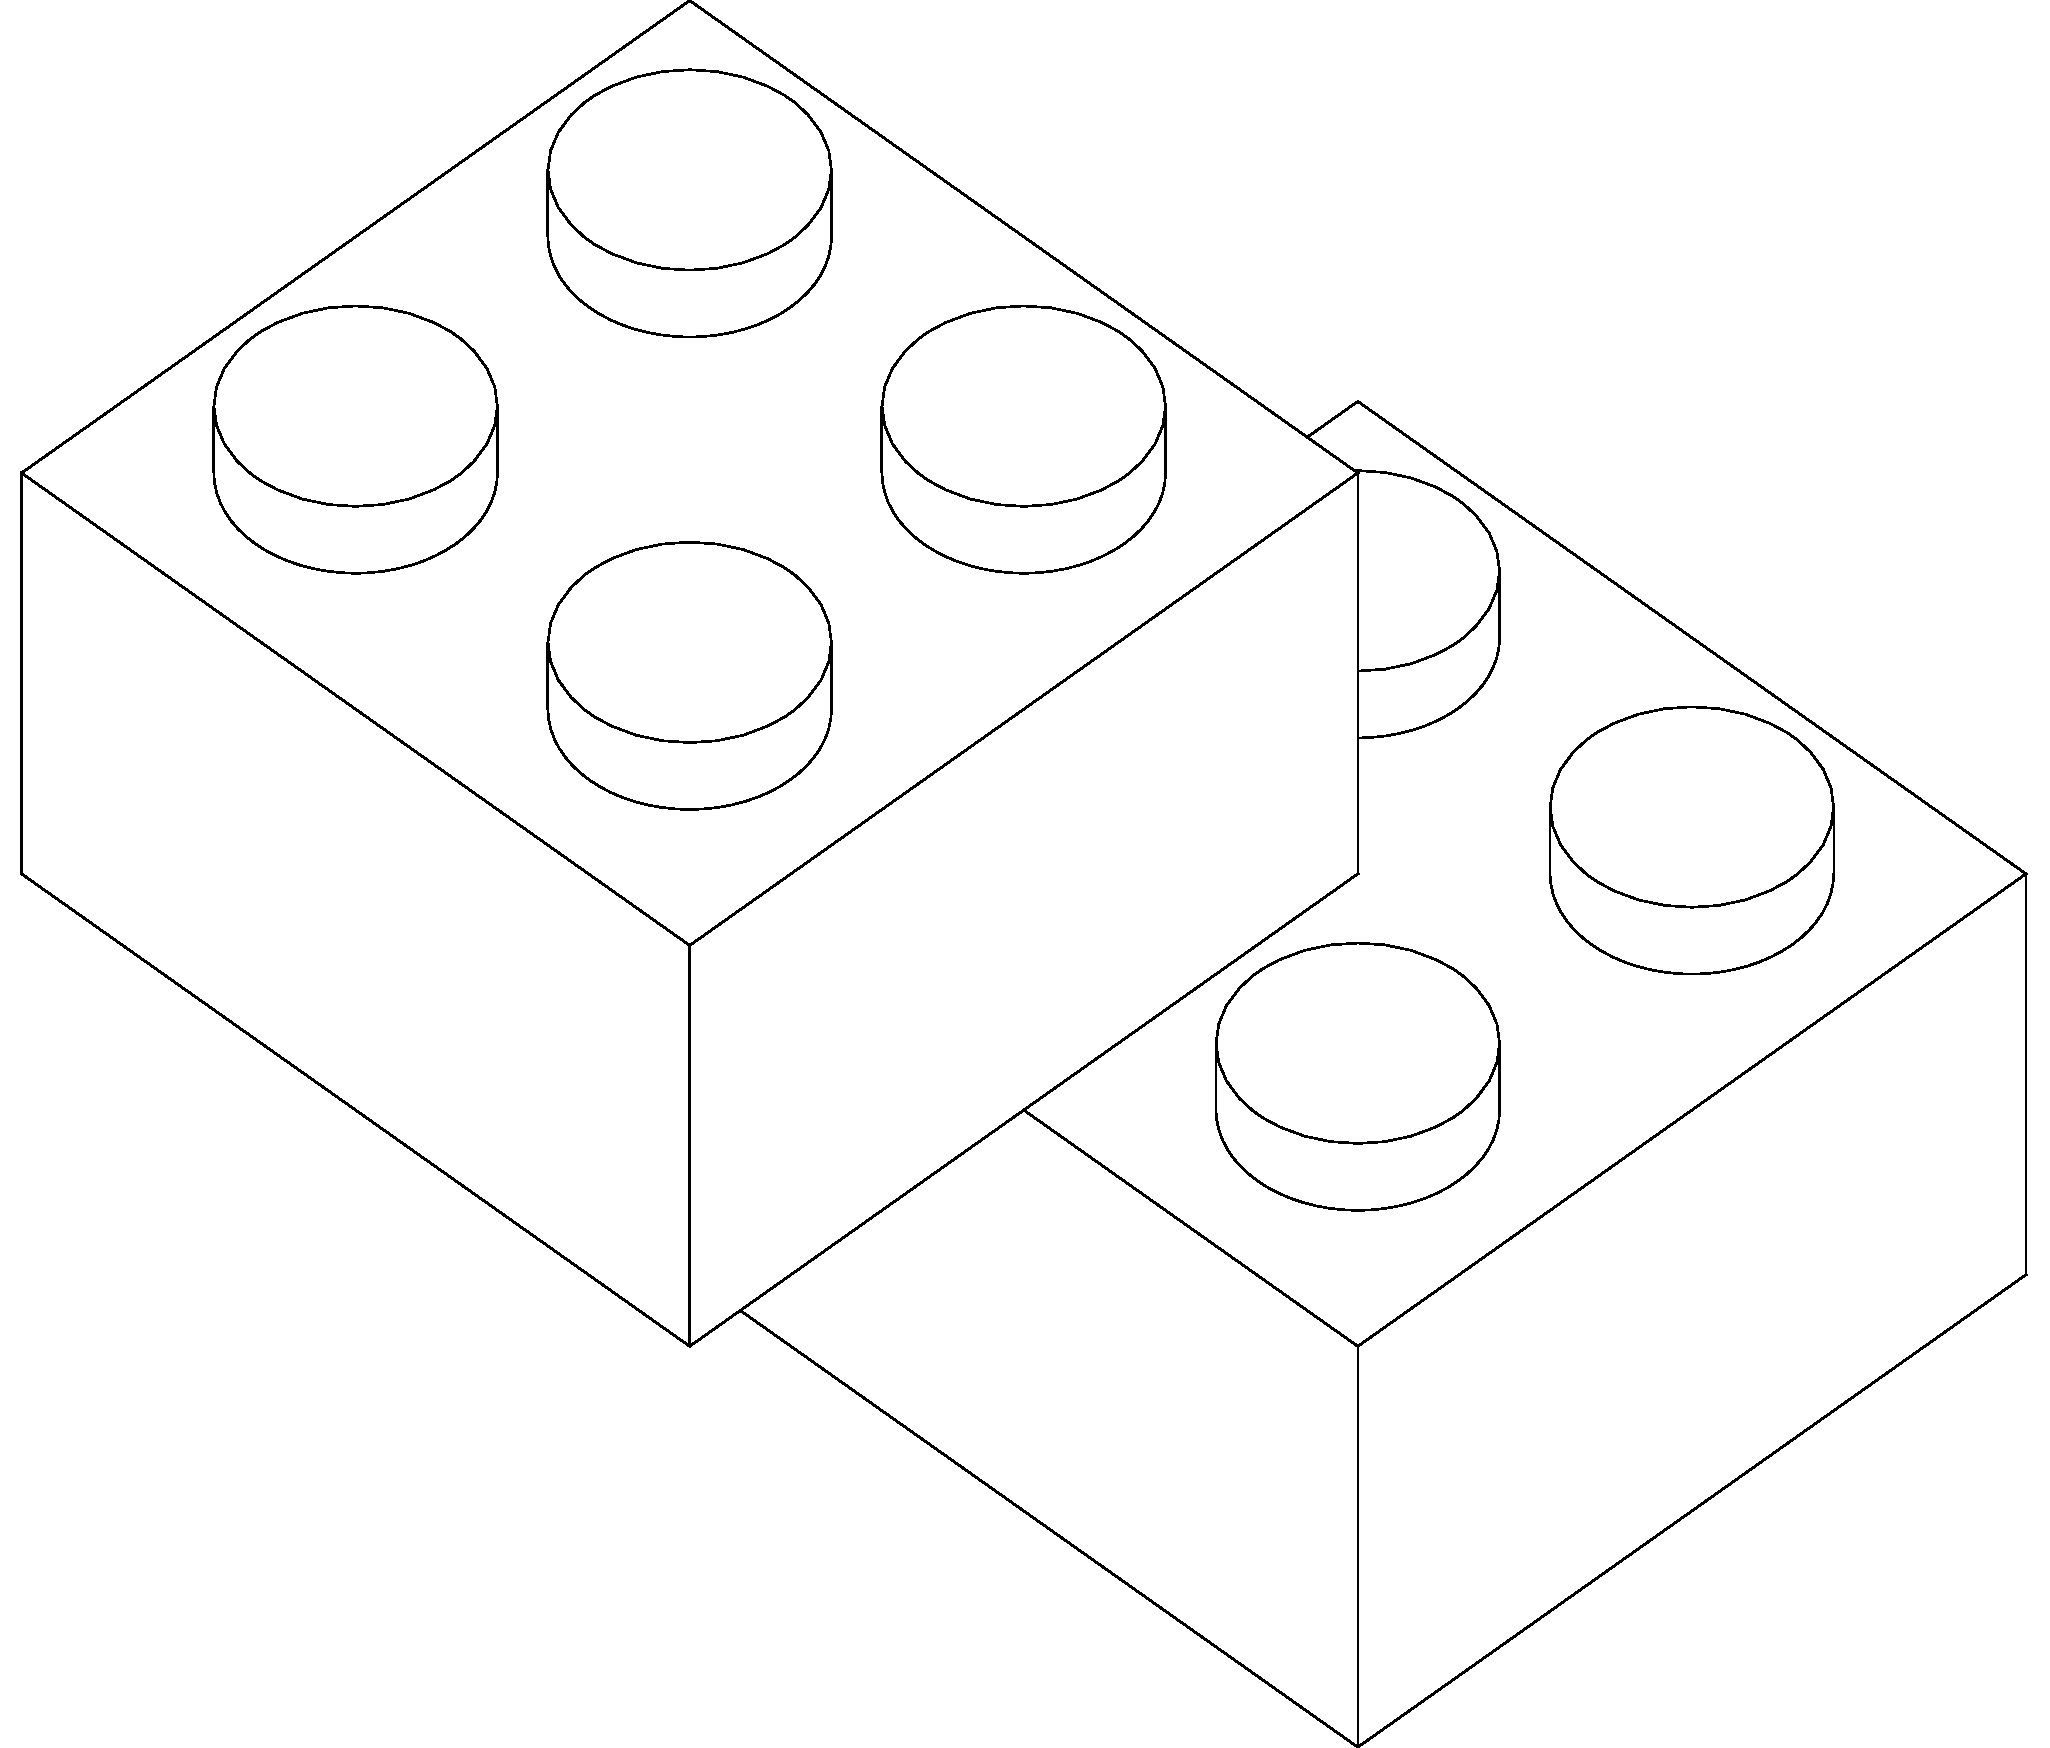
\includegraphics[height=4.5cm]{05_concept_generation/2x2-brick-combo-2.pdf}
    }
    \hfill
    \subfloat[Combination 3\newline Number of Pathways: 2]{
        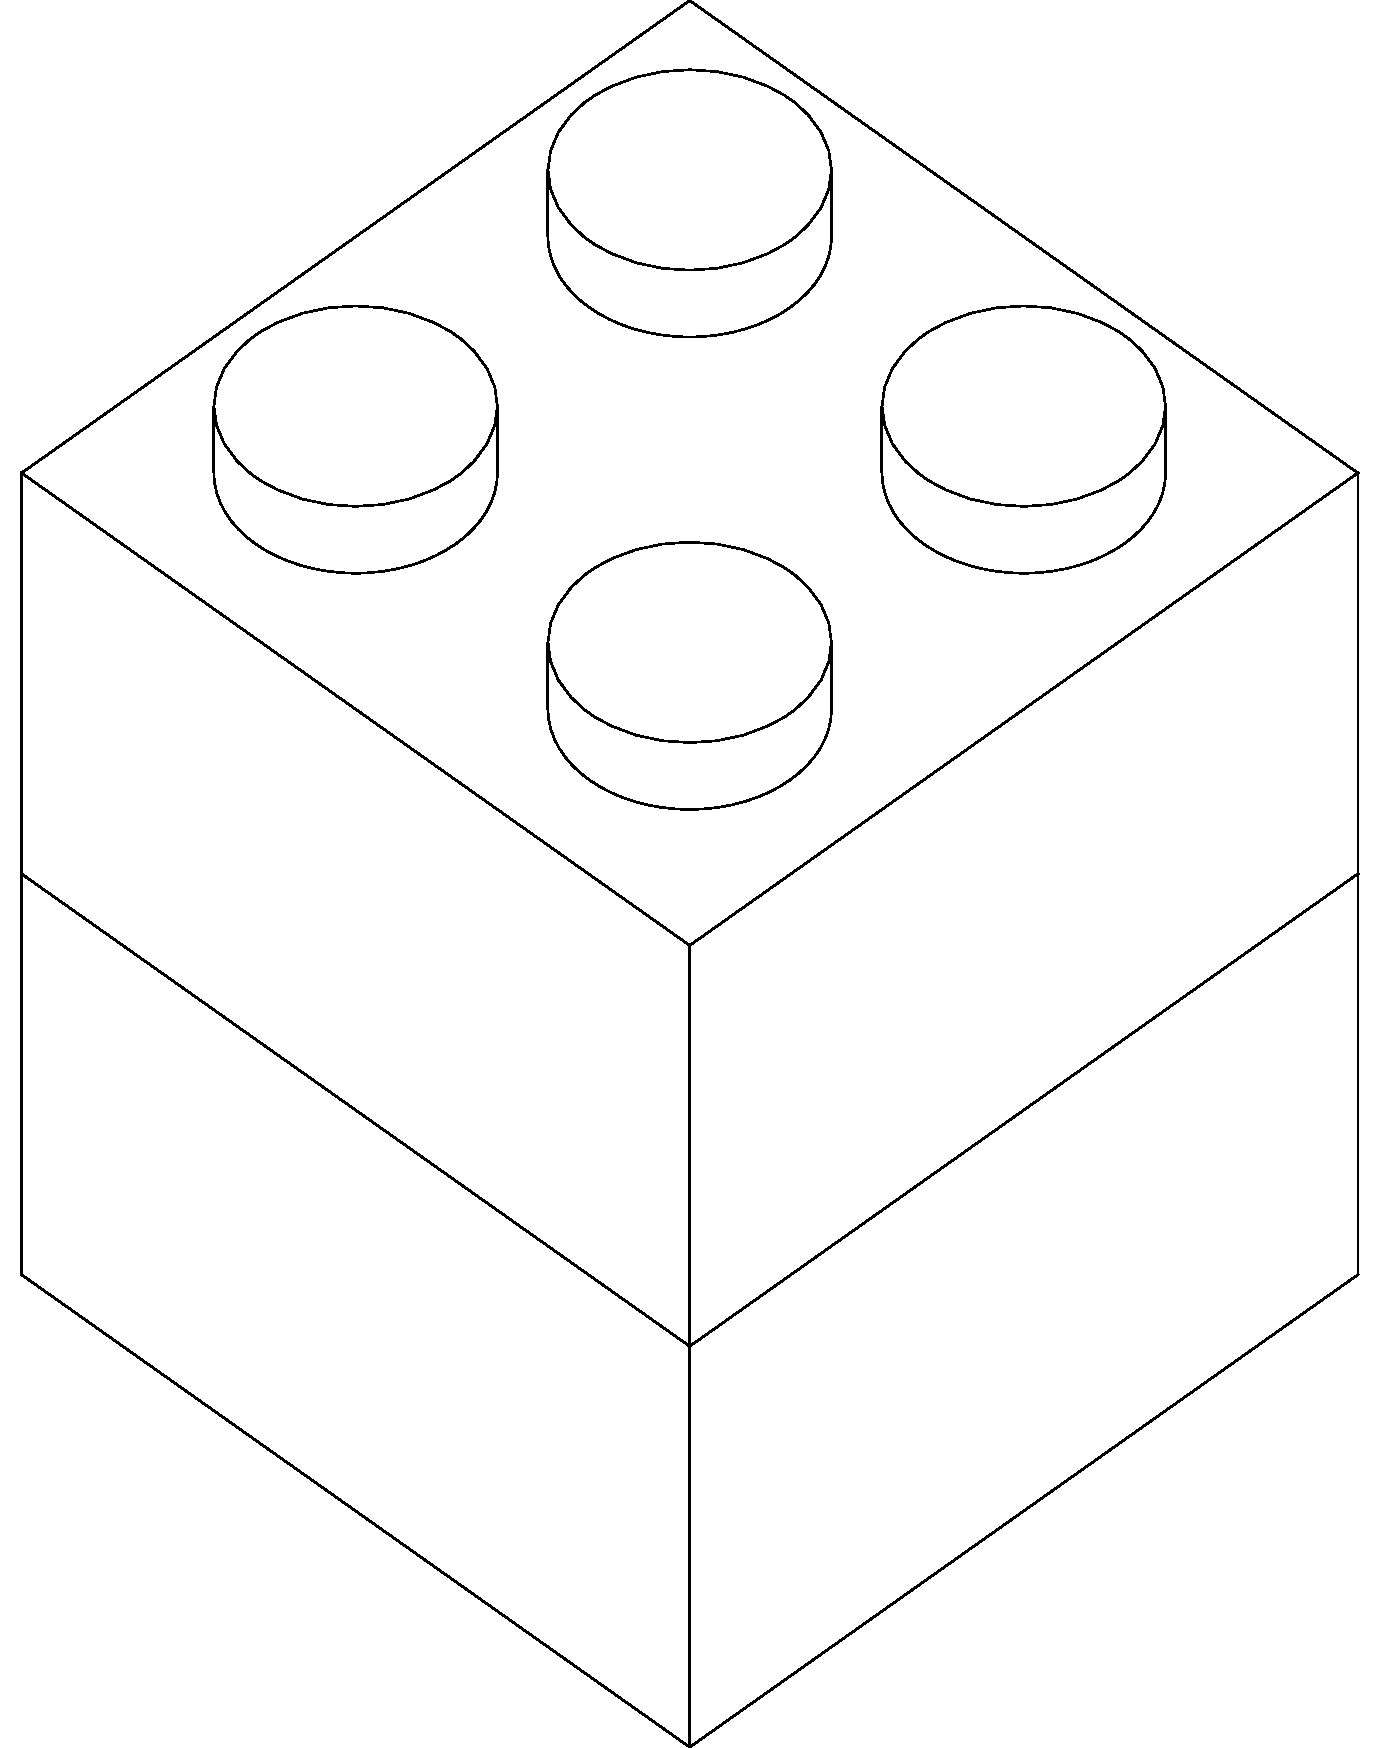
\includegraphics[height=4.5cm]{05_concept_generation/2x2-brick-combo-3.pdf}
    }
    %\hfill
    
    \vspace{2em}
    \caption{$B_{2,2}(2)$ combinations}
    \label{fig-combinations}
\end{figure*}

\section{Concept Selection} 

\newthought{Concept selection is the process} by which we decide upon the idea(s) that best satisfy the \ac{PDS}. These idea(s) are then selected for the detailed design stage.
It is important that we use a means that provides an unbiased systematic process to evaluating our concepts. In this section, we discuss four such methods.

\begin{enumerate}
    \item Controlled convergence
    \item Dot-sticking
    \item Multi-criteria decision analysis
    \item Weighted objectives tree
\end{enumerate}

\subsection{Controlled Convergence} Developed in the the 1980s by Stuart Pugh\cite{pugh1993}, Controlled Convergence uses a simple matrix to compare concepts against a set of pre-determined criteria.

\cref{tbl-controlled-convergence} provides an example of a controlled convergence matrix. The rows contain the requirements from the \ac{PDS} and each column represents one of the concepts that have been generated.

\begin{table}[ht!]
    \center
    \small
    \caption{Example of Controlled Convergence}
    \begin{tabular}{l c c c c}
        \toprule
        Criteria & Concept 1 & Concept 2 & Concept 3 & Concept 4 \\
        \midrule
        Ease of use &  & + & + & - \\
        Aesthetic appeal & D & - & + & + \\
        Manufacturability & A & + & + & - \\
        Low weight & T & + & - & + \\
        Energy efficiency & U & S & + & - \\
        Safety & M & - & + & S \\
        $\sum+$ & & 3 & 5 & 2 \\
        $\sum-$ & & 2 & 1 & 3 \\
        $\sum\text{S}$ & & 1 & 0 & 1 \\
        \midrule
        Net Score & 0 & 1 & 4 & -1 \\
        Rank & 3 & 2 & 1 & 4 \\
        \bottomrule
    \end{tabular}
    \label{tbl-controlled-convergence}
\end{table}

Taking one concept as a datum, we take the remaining concepts in turn and compare them to the datum with respect to each requirement. If the concept outperforms the datum on that criteria then a `$+$' should be placed in the table. A `$-$' if it under-performs and an `S' if it is the same as the datum. The assessment for each criteria can be subjective or objective. The important thing to remember is to record how you performed the assessment for each criteria.

Once all the concepts have been evaluated, the scores are tallied and the concepts ordered based on their rank. The concept with the highest score is usually taken forward but it is important to also reflect upon the matrix and see if their are any features that could be combined to develop a concept that is potentially more suited to the \ac{PDS}.

\subsection{Dot-Sticking}

Dot sticking \pref{fig-dot} is the method of voting for your preferred concept to carry forward. The reviewers of the concepts are provided with sticky dots (on-line forms are increasingly used) and they are asked to place the dot on their preferred concept. Each concept should be presented in the same manner so as to avoid bias in the selection process.

\begin{figure}[h!]
    \centering
    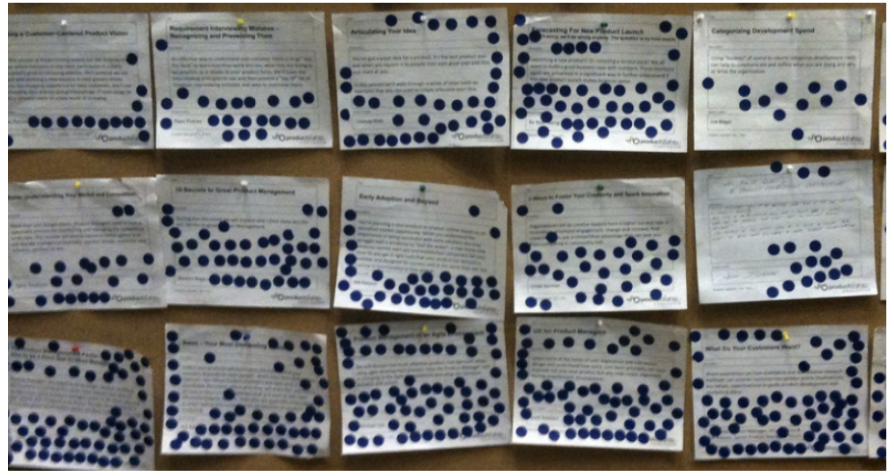
\includegraphics[width=0.95\textwidth]{06_concept_selection/dot-sticking.png}
    \caption{Dot sticking}
    \label{fig-dot}
\end{figure}

The technique is very simple and can be used to great effect when you need wider stakeholder engagement with the design process. In addition, it is very quick and can help reduce the number of concepts down to a small number in a short space of time. It is a very good tool to get initial feedback on the concepts you have generated.

\subsection{Multi-Criteria Decision Analysis}

\acf{MCDA} is very similar to the controlled convergence strategy in that it is a matrix formed of rows denoting your requirements and columns denoting your concepts. However, instead of using a datum concept, each concept is scored separately against the criteria and is typically performed using a Likert scoring scale (\cref{tbl-mcda}). Each requirement can also be weighted based on their priority/relative importance. The scores and weights are then summed to create an overall score for the concept. The concept with the greatest score is often considered the most suitable given the \ac{PDS}, but it is always important to reflect and investigate whether certain features of the other concepts can be merged/combined to generate a further, more refined concept.

\begin{table*}[h!]
    \centering
    \caption{MCDA comparing two potential projects}\label{tbl-mcda}
    \begin{tabular}{l l l l l l}
        \toprule
        & & \multicolumn{2}{c}{Project A} & \multicolumn{2}{c}{Project B} \\
        Criteria & Weighting & Score & Weighted & Score & Weighted \\
        \midrule
        Compatibility with strategic objectives & 7
        & 4
        & 28
        & 4
        & 28 \\
        High Market Value
        & 9
        & 4
        & 36
        & 4
        & 36 \\
        Genuine advantages over competition
        & 9
        & 4
        & 36
        & 5
        & 45 \\
        Generate or save large amounts of money
        & 10
        & 4
        & 40
        & 4
        & 40 \\
        Contact with the market
        & 8
        & 4
        & 32
        & 4
        & 32 \\
        Technical expertise available
        & 4
        & 5
        & 20
        & 3
        & 12 \\
        Commercial expertise available
        & 7
        & 1
        & 7
        & 1
        & 7 \\
        Project management resources available
        & 4
        & 3
        & 12
        & 3
        & 12\\
        Clear route for implementation
        & 4
        & 2
        & 8
        & 2
        & 8 \\
        Evolving/lurking risk factors
        & 6
        & 2
        & 12
        & 2
        & 12 \\
        Compliance with industry standards
        & 3
        & 2
        & 6
        & 2
        & 6 \\
        Total 
        & 450
        & 44
        & 292
        & 46
        & 317 \\
        \midrule
        \% of Total & & 65\% & & 70\% \\
        Rank & & 2 & & 1 \\
        \bottomrule
    \end{tabular}
    \vspace{1em}
\end{table*}

\marginnote[3em]{Pair-Wise Comparison} Applying weightings to the requirements can be a challenge but methods do exist to help us generate these weightings. Pair-wise comparison is one such method where you take each requirement and compare it with all the other requirements in your \ac{PDS}. You then determine which requirement is more important for your design. Performing this across all your requirements forms a matrix of comparisons. These can be re-ordered to highlight the order of priority of your requirements. Taking the most important requirement as the highest weighted requirement, all the other requirements can then be scaled to match.

\begin{table}
    \centering
    \caption{Pair-wise comparison for weighting requirements}
    \begin{tabular}{l l | l l l l l l l l l}
        \toprule
        Criteria & & A & B & C & D & E & F & G & H & I \\
        \midrule
        Functionality & A & - & A & C & D & A & F & A & AH & I \\
        Durability & B & - & - & C & D & B & B & B & H & BI \\
        Quality & C & - & - & - & D & C & F & C & H & C \\
        Affordability & D & - & - & - & - & D & F & D & D & I \\
        Manufacturability & E & - & - & - & - & - & F & E & H & E \\
        Usability & F & - & - & - & - & - & - & F & FH & I \\
        Maintainability & G & - & - & - & - & - & - & - & H & I \\
        Safety & H & - & - & - & - & - & - & - & - & I \\
        Marketability & I & - & - & - & - & - & - & - & - & - \\
        \bottomrule
    \end{tabular}
\end{table}

\subsection{Weighted Objectives Tree}

The Weighted Objectives Tree approach focuses on unpacking the design brief into lower-level requirements that can be assessed or measured through either quantitative and qualitative techniques \pref{fig-wot}. 
Weighted Objectives Trees are particularly useful for highly-complex and inherently hierarchical products.

\begin{figure*}[h!]
    \centering
    \includestandalone[width=\textwidth, mode=buildnew]{06_concept_selection/weighted_objectives_tree}
    \vspace{1em}
    \caption{Weighted objectives tree}
    \label{fig-wot}
\end{figure*}

The high-level objective is usually given a weighting of 1.0.
This value of unity has to be split amongst the next level of objectives.
Taking the example in \cref{fig-wot}, it was decided that reliability was more important than low-mass and compactness by a factor of 0.5 to 0.3 to 0.2.

These relative weightings have to be multiplied by the value of the weighting in the next level up to get the absolute weightings.
Since the objective at the next level up has a value of unity, the absolute weightings are still 0.5, 0.3 and 0.2.
This process is followed down to all the root-objectives. 

At any particular level the relative weightings always add up to 1.0.
The absolute weightings get smaller and smaller as the tree goes down to lower levels.
By definition, the sum of the absolute weightings of all the root objectives must come to exactly 1.0.

%\subsection{This Design Exercise}

%In this design exercise, we would like you to follow the \ac{MCDA} method for selecting the concept that you will be taking forward. You should discuss the \ac{MCDA} method in your report and how you have applied it in your case. There should also be a discussion of the results and if there has been any consideration on merging features from multiple concepts.

%Remember to try and make quantifiable comparisons as much as possible and we will be expecting you to perform some calculations in terms of areas and potential masses for each of the concepts.


\section{Design for X}

\newthought{\acf{DfX}} concerns the development of guidelines and principles that support engineers in developing optimised products for a particular area. Examples include the Design for:

\begin{multicols}{2}
    \begin{itemize}
        \item Additive (3D Printing)
        \item Assembly
        \item Environment
        \item Disassembly
        \item Manufacturing
        \item Inspection
        \item Safety
        \item Service
        \item Six Sigma
    \end{itemize}
\end{multicols}


It is not uncommon for a products design to go through a number of iterations where the engineering design team will focus on a particular \ac{DfX} element.
Over the course of the design, compromises will have to be made to develop a product that meets all these requirements.

In this exercise, we will focus on principles around \acf{DfA} and \acf{DfM}.
Successful \ac{DfA} and \ac{DfM} activities will reduce the material, overhead and labour costs incurred when producing the product.
Remember, 70-80\% of the committed cost is made at the design stage!\cite{ullman2002}\cite{corbett1986}\cite{mileham1993}

\acf{DfA}\marginnote{Design for Assembly} covers the principles and techniques that support the development of a design that is easy to assemble. Significant reductions in cost and the number of parts required to produce a product can be achieved through using these techniques.

Thus, \ac{DfA} is mainly concerned with minimising the number of assembly operations.
This is often achieved by reducing the part count by combining part geometries together in order to increase their functionality.
It is therefore common to see a decrease in parts and increase in part complexity after a \ac{DfA}  exercise is performed on a product. 

\acf{DfM}\marginnote{Design for Manufacture} covers the principles and guidelines that support designers in selecting an appropriate manufacturing technique for a component and optimising a components geometry for a particular technique. Optimising a design for manufacture can greatly reduce manufacturing lead-times and production costs. 

In this exercise, you will be using the tools available in the student workshops, rapid prototyping tools including laser cutting and 3D printing, and buying in standard components. The following sections will cover:

\begin{itemize}
    \item Design for (Manual) Assembly
    \item Design for Manufacture (Laser Cutting)
    \item Design for Manufacture (3D Printing)
\end{itemize}

Although we are focusing on laser cutting and 3D printing technologies in these course notes.
You should also be looking back at your student workshop experience and bring that knowledge to bear on the development of the manufacturing processes for your components.
So remember to think about the use of:

\begin{itemize}
    \item Hand-tools;
    \item Lathes;
    \item Pillar drills; and,
    \item CNC machining in your design.
\end{itemize}

\subsection{Design for (Manual) Assembly}

Before\marginnote{principles for DfA.\\\noindent\normalfont Acknowledgements to \citet{boothroyd2011} and Stienstra's Lecture on an ``Introduction to Design for (Cost Effective) Assembly and Manufacturing''.} one starts out on a DfA activity, there is a need to identify the aims and objectives of the activity to ensure that we can assess the output.
For DfA, engineers often aim to:

\begin{itemize}
    \item Minimise part count
    \item Design parts with self-locating features
    \item Design parts with self-fastening features
    \item Minimise the re-orientation of parts during assembly
    \item Design parts for retrieval, handling \& insertion
    %\item Emphasise the application of `top-down' assembleis
    \item Standardise parts and minimise the number of fasteners
    \item Encourage modularisation to enable parallel assembly
    \item Introduce symmetry to increase the number of orientations available for assembly
\end{itemize}

However, the aims and objectives may differ for your exercise so remember to look at the context of the design problem and see how these aims might help or hinder the progress of your design. In your case, remember that you're building a prototype of your design so you may want to ensure there is flexibility in the positioning of components in case some of your calculations have any errors as well as the manufacturing tolerances from techniques that will be employed.

With\marginnote{the DfA activity} the aims set, we can now proceed to assess the designs ability to be assembled. In the case of this exercise, we will follow a four step procedure:

\begin{description}
    \item[Step 1] Functional analysis of the design
    \item[Step 2] Estimating Assembly Time
    \item[Step 3] Applying Design for Manual Assembly Guidelines
    \item[Step 4] Compare the new design to the old design
\end{description}

To\marginnote{Step One} start, we form a spreadsheet of all the parts in the current design and if possible, place them within their potential sub-assemblies. Once all the parts have been listed, we then determine the number of parts ($N_p$) and number of interfaces ($N_i$) these parts have with one another. 

Now it is time to determine whether a part is essential to the designs function or not and this can be achieved by asking the questions outlined in the functional analysis chart \pref{fig-functional}. 

\begin{figure*}[h!]
    \centering
    \includestandalone[width=0.9\textwidth, mode=buildnew]{07_design_for_x/functional_analysis_chart}
    \vspace{1em}
    \caption{Functional Analysis Chart}\label{fig-functional}
\end{figure*}

Alongside this, we need to assess whether there are any components that can be further standardised within the products. The level of standardisation is not critical at the moment and could be at the assembly, full assembly, assembly plant, corporation or industry levels. Then there is the question as to whether the part should be standardised. A `Yes' should only be placed next to part if both these criteria are met.

Having\marginnote{Part Count Efficiency $(\eta_{\text{part count}})$} calculated these values, we can begin to assess the performance of our current design. One metric that we use to assess a design is on it's part count efficiency. This is defined as the ratio between the theoretical number of parts required for the product to perform its function and actual number of parts within the design \pref{equ-part-eff}.

\begin{equation}
    \eta_{\text{part count}} = \frac{\sum{N_\text{essential}}}{\sum{N_p}}
    \label{equ-part-eff}
\end{equation}

It is common that the designs following a DfA will have $\eta_{\text{part cout}}>0.6$ and this is the value that we will use as our objective.

In\marginnote{DfA Complexity Factor} addition to part count efficiency, we have the \ac{DfA} complexity factor, which is based on the number of parts and interactions within the design. It is calculated as the square root of the number of parts multiplied by the number of interactions.

\begin{equation}
    \text{Complexity Factor} = \sqrt{\sum{N_p}\times\sum{N_i}}
\end{equation} 


The objective of \ac{DfA} is to reduce this value, which can be achieved by reducing both the number of parts and interactions within the product. \cref{tbl-parts} shows an example output of Step 1.

\begin{table}[h!]
    \centering
    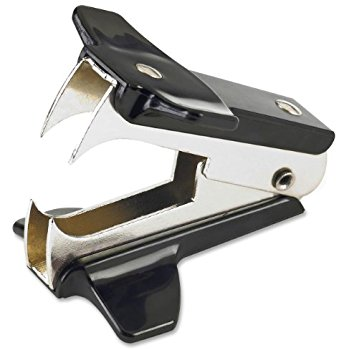
\includegraphics[width=0.3\textwidth]{07_design_for_x/staple-remover.jpg} \\
    \footnotesize
    \begin{tabular}{l l r r c c}
        \toprule
          Part No. & Part Name & $N_p$ & $N_i$ & Essential &Standardised? \\
        \midrule
          1. & Lower Arm Sub-Assembly \\
        \midrule
          1.1 & Lower Arm & 1 & 6 & Y & N \\
          1.2 & Lower Arm Cover & 1 & 3 & N & Y \\
          1.3 & Rivet & 2 & 4 & N & N \\
        \midrule
          2. & Upper Arm Sub-Assembly & & \\
        \midrule
          2.1 & Upper Arm & 1 & 6 & N & N \\
          2.2 & Upper Arm Cover & 1 & 3 & N & Y \\
          2.3 & Rivet & 2 & 4 & N & N \\
        \midrule
          3. & Spring & 1 & 3 & N & N \\
        \midrule
          4. & Pivot & 1 & 3 & N & N \\
        \midrule
          Totals & & 10 & 32 & 1 & 2 \\
        \bottomrule
    \end{tabular}
    \caption{Staple remover functional analysis}\label{tbl-parts}
\end{table}


With\marginnote{Step Two} the functional analysis of the product complete, the next step is to calculate the assembly time for the product. This is not too much of a problem when you have an existing design that you're already manufacturing but can be challenging to estimate when you're early in the conceptual design phases.

To help us with determining the assembly time of components, researchers have performed studies into the time taken to perform common assembly tasks such as screwing components together, inserting bolts and handling time for small components. Figure~\ref{fig-screw} provides one such example.

\begin{figure}
    \centering
    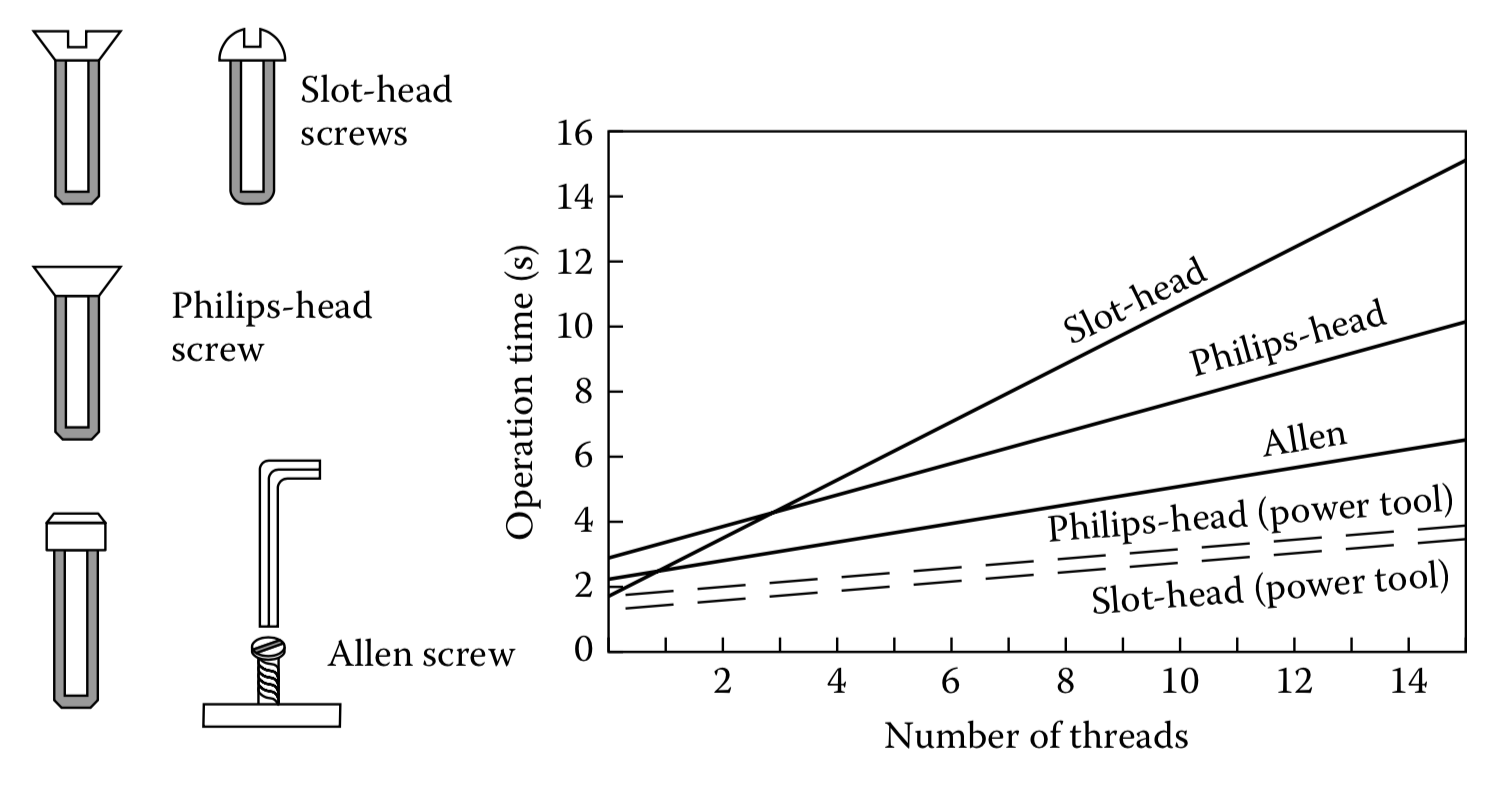
\includegraphics[width=\textwidth]{07_design_for_x/screwing.png}
    \caption[Effect of number of threads on time to pick up the tool, engage the screw, tighten the screw, and replace the tool]{Effect of number of threads on time to pick up the tool, engage the screw, tighten the screw, and replace the tool~\citep{boothroyd2011}.}\label{fig-screw}
\end{figure}


From these charts, we can build an estimate for the assembly time for the current design. This forms the baseline that we can use to compare future iterations against.

\marginnote{Assembly Index} The assembly time can also be used to calculate the assembly index and is an indicator of the efficiency of the assembly process by comparing it to a theoretical minimum assembly time. This is obtained by multiplying the theoretical minimum part count of four by a minimum time of assembly for each part of 3s. 

\begin{equation}
  \text{Assembly index} = \frac{3\sum{N_i}}{\text{Assembly time}}
\end{equation}


With\marginnote{Step Three} our baseline set, we can begin to analyse and generate ideas of how we can improve the design for assembly. Step 3 is where we apply the \ac{DfA} guidelines to the current design and see if improvements can be made to ease its assembly.

It\marginnote{Component Elimination} is a rule of thumb that if a third of the components in a product are fasteners then one should look at the method of assembly. \cref{fig-bracket} shows an example of a roll-bar redesign where the number of parts has been reduced from 25 to 14.

\begin{figure*}[t!]
  \centering
  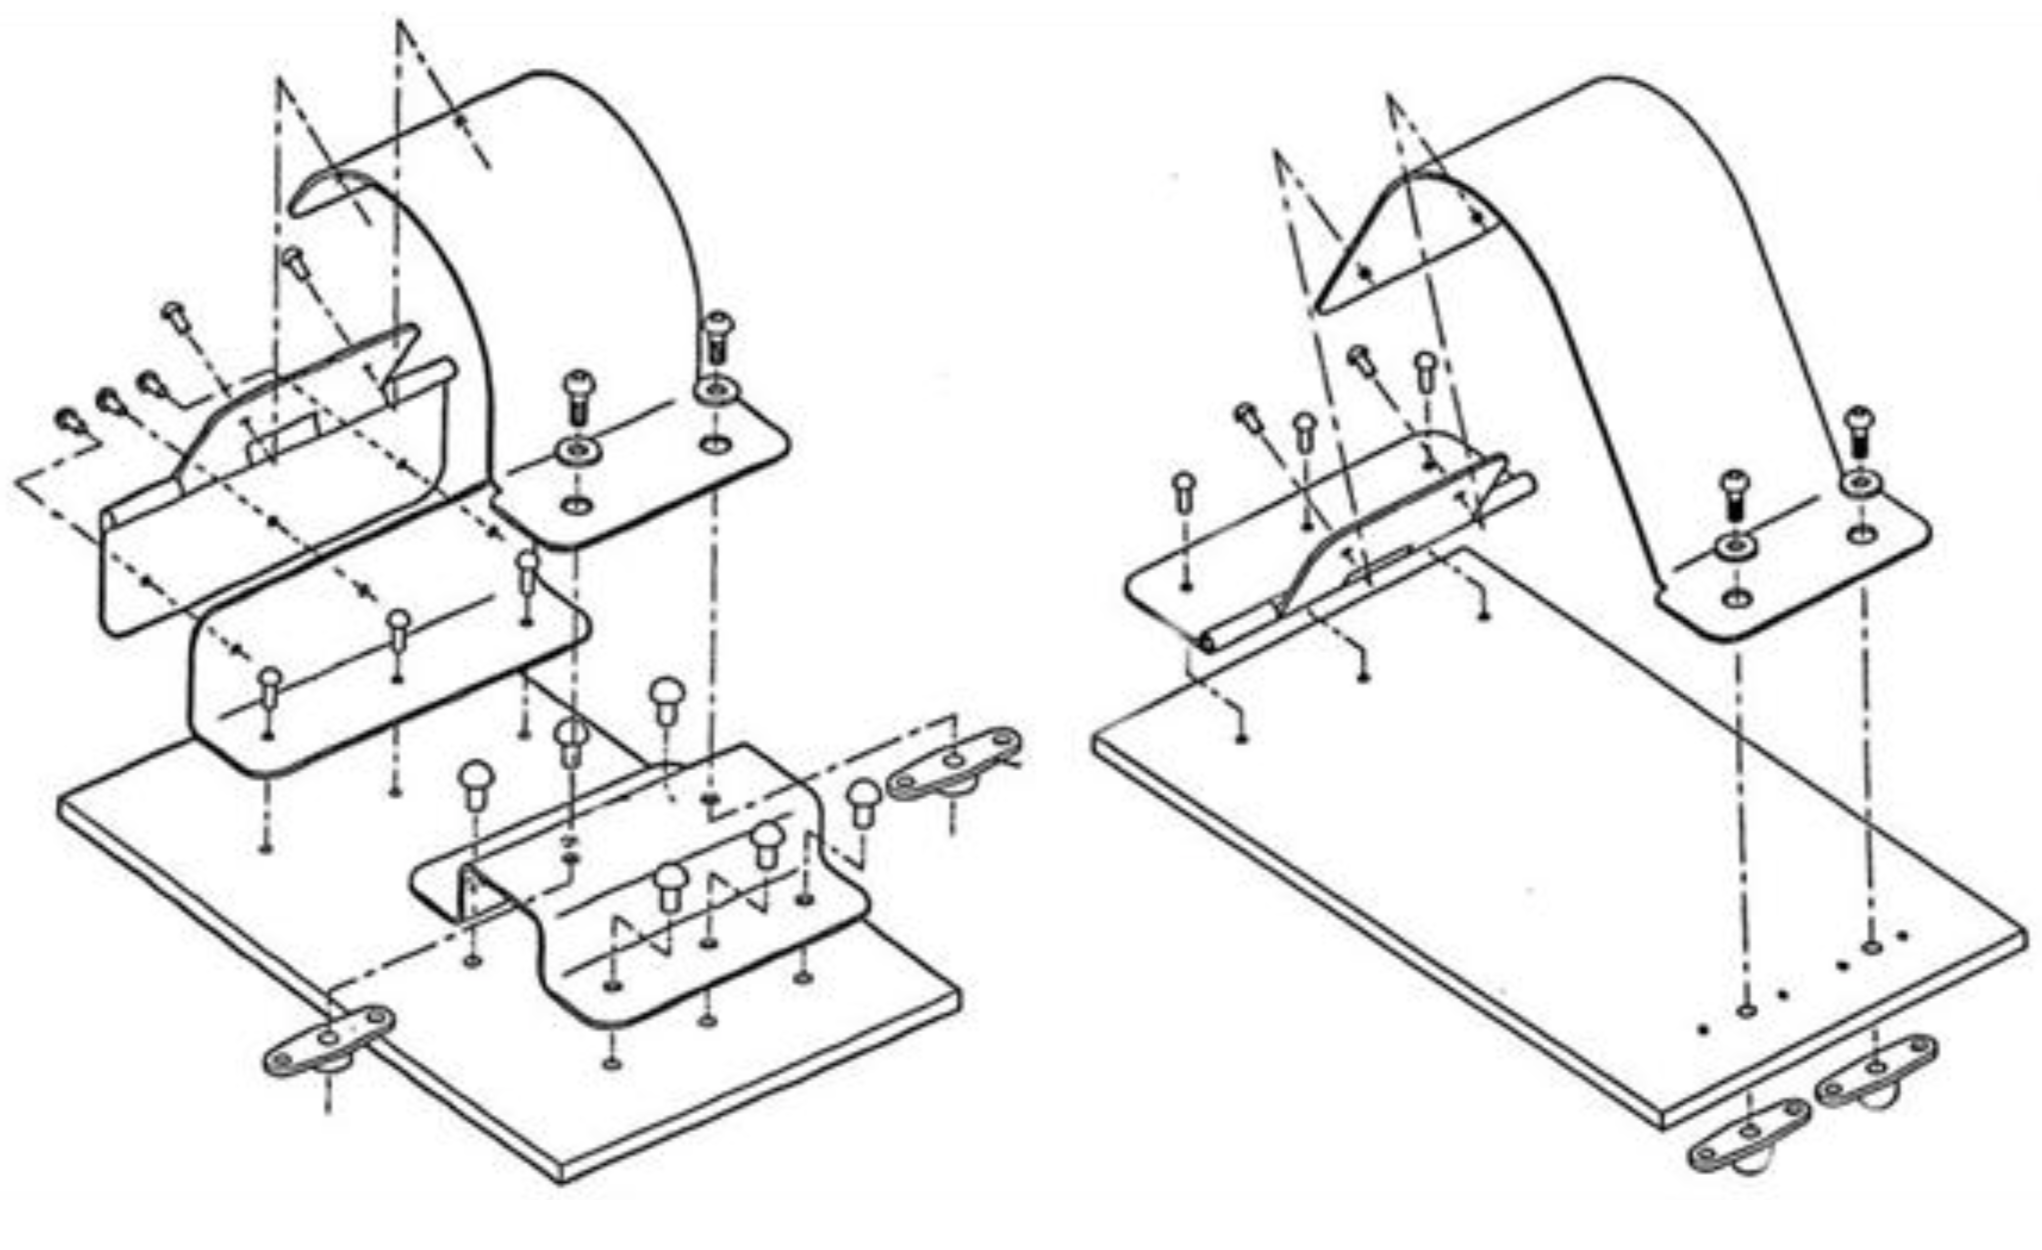
\includegraphics[width=0.8\textwidth]{07_design_for_x/simplification.png}
  \caption{Simplification of a sheet metal bracket}\label{fig-bracket}
\end{figure*}


Remember, eliminated parts never need to be:

\begin{multicols}{3}
    \begin{itemize}
        \item Designed
        \item Detailed
        \item Prototyped
        \item Produced
        \item Scrapped
        \item Tested
        \item Re-engineered
        \item Purchased
        \item Progressed
        \item Received
        \item Inspected
        \item Rejected
        \item Stocked
        \item Outdated
        \item Written-off
        \item Unreliable
        \item Recycled
        \item Late
    \end{itemize}
\end{multicols}

However\marginnote{Standard Sizes}, there are times when fasteners are required and the number cannot be reduced further. In these cases, it is worth checking whether the types of fastener (e.g.\ bolt size) can be reduced. It is much easier for a company to stock one type of bolt than it is a hundred and simplifies the assembly time as there is less chance the wrong bolt is selected to mate two parts.

Fasteners\marginnote{Fastener Cost} also have an inherent cost in terms of the time it takes to assemble a component with them. Some of the lowest cost fasteners are snap fits requiring very little time and effort use. Whilst bolting requires additional equipment and many turns until the two parts are assembled. In addition, they may be the need to torque the bolt to a specific level, which further increases the assembly time.

In\marginnote{Part Handling} general, for ease of part handling, a design engineer should attempt to:

\begin{enumerate}
    \item Design parts that have an end-to-end symmetry and rotational symmetry about the axis of insertion. If this cannot be achieved, try to design parts having the maximum possible symmetry (\cref{fig-handling}a).
    \item Design parts that, in those instances where the part cannot be made symmetric, are obviously asymmetric (\cref{fig-handling}b).
    \item Provide features that prevent jamming of parts that tend to nest or stack when stored in bulk (\cref{fig-handling}c).
    \item Avoid features that allow tangling of parts when stored in bulk (\cref{fig-handling}d).
    \item Avoid parts that stick together or are slippery, delicate, very small or very large, or that are hazardous to the handler (i.e.\ parts that are sharp, splinter easily, etc.)
\end{enumerate}

\begin{figure}[t!]
    \centering
    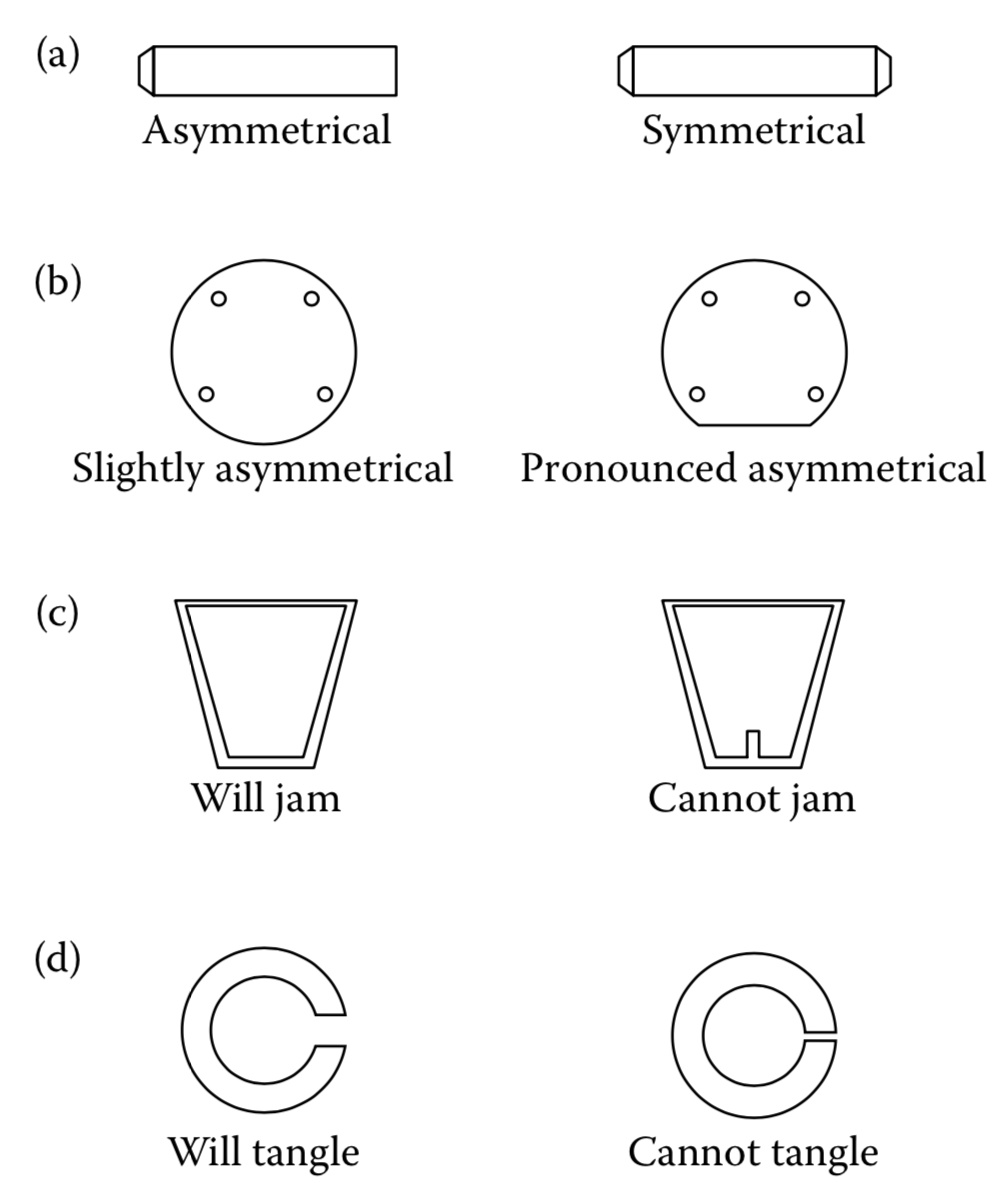
\includegraphics[width=0.6\textwidth]{07_design_for_x/handling.png}
    \caption[Geometric features that effect part handling]{Geometric features that effect part handling~\citep{boothroyd2011}.}\label{fig-handling}
\end{figure}

\marginnote{Insertion and Fastening} For ease of insertion, an engineer should attempt to:

\begin{enumerate}
    \item Design so that there is little or no resistance to insertion and provide chamfers to guide the insertion of two mating parts. Generous clearance should be provided, but care must be taken to avoid clearances that result in a tendency for parts to jam or hang-up during insertion.
    \item Standardize by using common parts, processes, and methods across all models and even across product lines to permit the use of higher volume processes that normally result in lower product cost.
    \item Use pyramid assembly to provide progressive assembly about one axis of reference. In general, it is best to assemble from above.
    \item Avoid, where possible, the necessity for holding parts down to maintain their orientation during manipulation of the sub-assembly or during the placement of another part. If holding down is required, then try to design so that the part is secured as soon as possible after it has been inserted.
    \item Design so that a part is located before it is released. A potential source of problems arises from a part being placed where, due to design constraints, it must be released before it is positively located in the assembly. Under these circumstances, reliance is placed on the trajectory of the part being sufficiently repeatable to locate it consistently.
    \item When common mechanical fasteners are used, the following sequence indicates the relative cost of different fastening processes, listed in the order of increasing manual assembly cost.
    \begin{enumerate}
        \item Snap fits
        \item Plastic bending
        \item Riveting
        \item Screw fastening
    \end{enumerate}
    \item Avoid the need to re-position the partially completed assembly in the jig.
\end{enumerate}

By\marginnote{Step Four} evaluating your designs with respect to these guidelines, new design should emerge that will ease the assembly of the product. To evaluate the relative success of the DfA activity, we now perform Steps 1 \& 2 again for the new design and compare it with the old version.

To demonstrate the potential improvements that can be gained by performing this activity, \cref{fig-motor} illustrates the design changes that were made to a motor drive assembly.
And, \cref{tbl-comparison} shows the comparison of the original motor design against the re-design motor assembly.
The results show a:

\begin{itemize}
    \item 68\% reduction in the number of parts required;
    \item 70\% reduction in assembly time; and,
    \item 71\% reduction in labour costs.
\end{itemize}


\begin{figure*}[ht!]

    \hfill
    \subfloat[Original design]{
        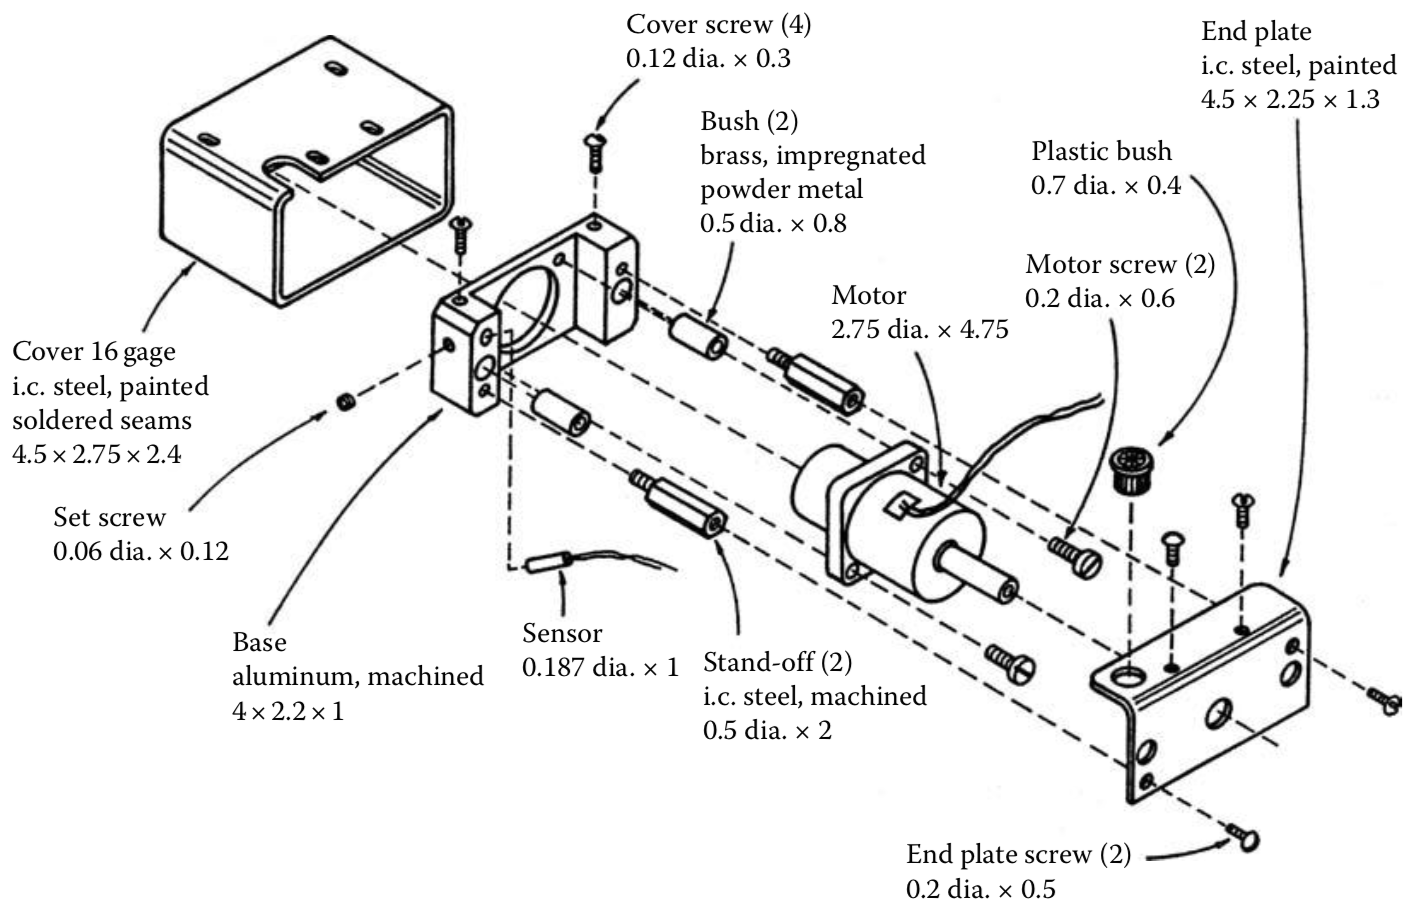
\includegraphics[width=0.43\textwidth]{07_design_for_x/motor-1.png}
    }
    \hfill 
    \subfloat[Re-design]{
        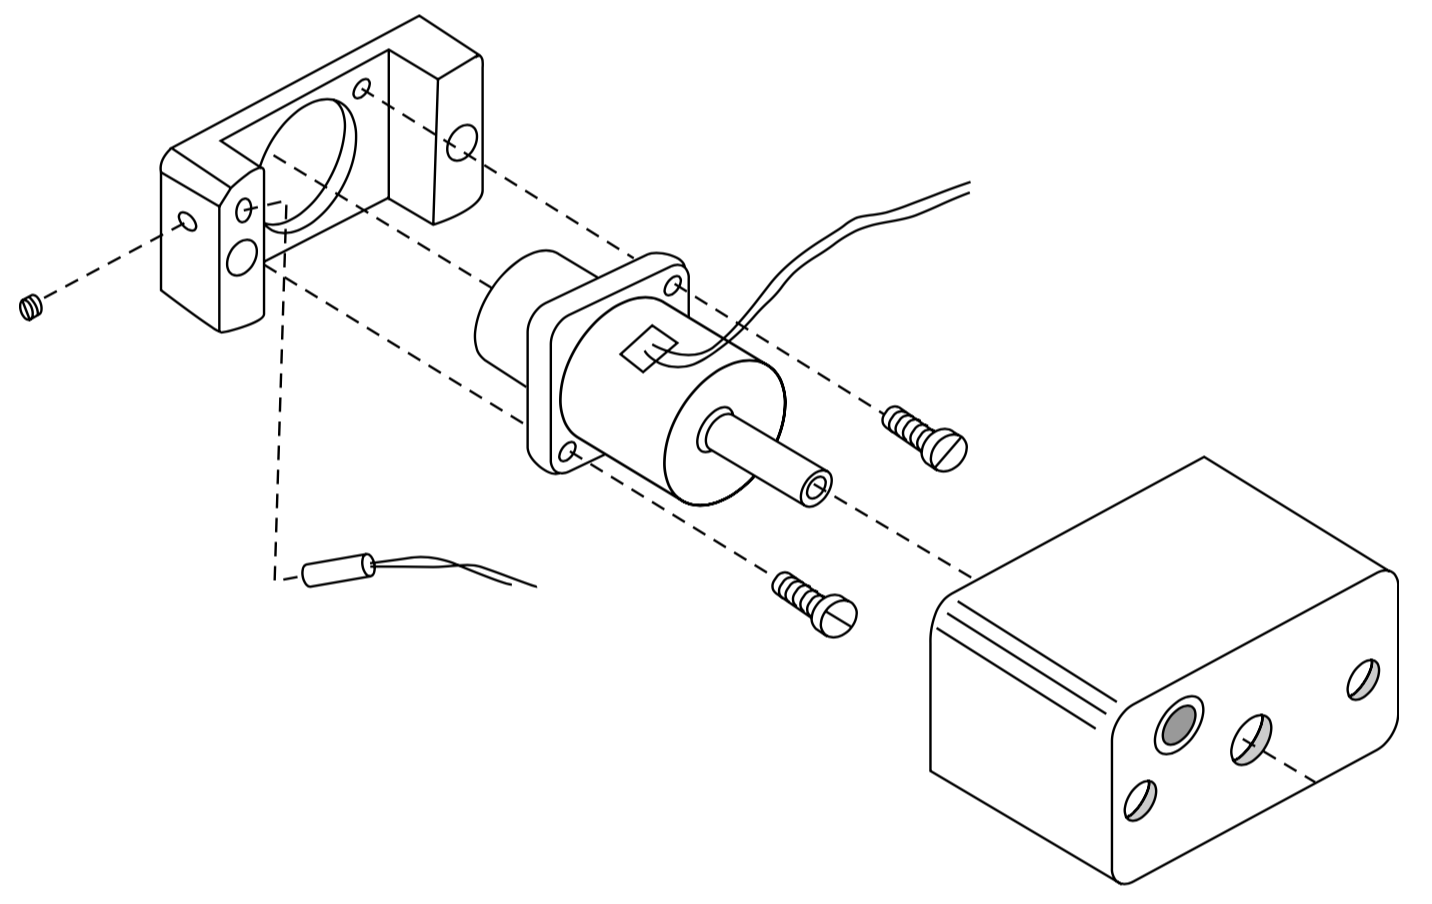
\includegraphics[width=0.43\textwidth]{07_design_for_x/motor-2.png}
    }
    \hfill
    
    \vspace{1em}
    \caption{Motor drive assembly DfA re-design}\label{fig-motor}
\end{figure*}

\begin{table*}[ht!]
    \centering
    \resizebox{\textwidth}{!}{
    \scriptsize
    \begin{tabular}{l | r r | r r | r r | r r}
      \toprule
        Part & \multicolumn{2}{c|}{$N_p$} & \multicolumn{2}{c}{$N_i$} & \multicolumn{2}{c}{Assembly Time (s)} & \multicolumn{2}{c}{Assembly Cost (\textdollar)*} \\
        & Original & Re-Design & Original & Re-Design & Original & Re-Design & Original & Re-Design \\
      \midrule
        Base & 1 & 1 & 1 & 1 & 3.5 & 3.5 & 2.9 & 2.9 \\
        Bushing & 2 & -- & 0 & -- & 12.3 & -- & 10.2 & -- \\
        Motor sub-assembly & 1 & 1 & 1 & 1 & 9.5 & 4.5 & 7.9 & 3.8 \\
        Motor screw & 2 & 2 & 0 & 0 & 21.0 & 12.0 & 17.5 & 10.0 \\
        Sensor sub-assembly & 1 & 1 & 1 & 1 & 8.5 & 8.5 & 7.1 & 7.1 \\
        Set screw & 1 & 1 & 0 & 0 & 10.6 & 8.5 & 8.8 & 7.1 \\
        Standoff & 2 & -- & 0 & -- & 16.0 & -- & 13.3 & -- \\
        End plate & 1 & -- & 1 & -- & 8.4 & -- & 7.0 & -- \\
        End plate screw & 2 & -- & 0 & -- & 16.6 & -- & 13.8 & -- \\
        Plastic bushing & 1 & -- & 0 & -- & 3.5 & -- & 2.9 & -- \\
        Thread leads & -- & -- & -- & -- & 5.0 & 5.0 & 4.2 & 4.2 \\
        Reorient & -- & -- & -- & -- & 4.5 & -- & 3.8 & -- \\
        Cover & 1 & 1 & 0 & 1 & 9.4 & 4.0 & 7.9 & 3.3 \\
        Cover screw & 4 & -- & 0 & -- & 31.2 & -- & 26.0 & -- \\
        \midrule
        Totals & 19 & 6 & 4 & 4 & 160.0 & 46.0 & 133.0 & 38.4 \\
      \bottomrule
      \multicolumn{5}{l}{*labour cost at \textdollar30ph} \\
    \end{tabular}
    }
    \vspace{1em}
    \caption{Motor DfA comparison}
    \label{tbl-comparison}
\end{table*}


\subsection{Design for Manufacture (Laser Cutting)}

Laser\marginnote{\normalfont Acknowledgements to Sculpteo's ``Laser Cutting: The Ultimate Guide''} cutting works by directing the output of a high-power laser through optics. They direct the laser beam generated on a small zone of the material. The material then either melts, burns, vaporizes away, or is blown away by a jet of gas, leaving an edge with a good quality surface finish. Typical prototyping laser cutters can cut up to \SI{20}{\milli\metre} thick material.

Laser cutting machines function from digital orders, based on the topographic information contained in a 2-D vector file. They cut or engrave the material plate in different locations, thus allowing an item's surface to be delineated and decorated.

\subsubsection{Origins of Laser Cutting}

One\marginnote{1965} of the earliest known applications of laser technology in manufacturing was as a cutting device for electrical connections. This had been previously achieved through diamond dies and many thousands were used in the process. Diamond dies were both costly and time consuming to make. Cutting with laser technology overcame this barrier but there were still concerns over its safety.

In 1967\marginnote{1967}, Peter Houldcroft of the The Welding Institute in Cambridge discovered that combining a focused laser beam with an oxygen assist gas could improve the precision and speed by the cutting process. This led to the development of the laser cutting nozzle we know today\cite{sullivan1967}.

Industrial\marginnote{1969} application of laser cutting technologies started to be realised with Boeing becoming one of the first to integrate the technology within its production lines. The focus was on the development of the technology to cut `hard' material such as titanium, hastelloy and ceramic. There results led to the patenting of multi-beam laser cutting.

Now\marginnote{1979} laser cutting had become synonymous of cutting in two dimensions and it wasn't until 1979 when Italian company Prima Industrie demonstrated that it was possible to use the technology in a three-dimensions by placing the process on a 5-axis rotation system.

Fast\marginnote{Today} forward to today and laser cutters have fully-established themselves as a viable manufacturing technology in both prototyping and production. The technology has also shrunk to the size that you can fit one on your desktop. It is used in a range of sectors including marketing, solar panel construction and aerospace. And now in the Design \& Make exercise!

\subsubsection{Laser Cutting Process}

\cref{fig-cutter} shows a schematic of the laser cutting process. The laser originates from a laser resonator, which sends out a beam of intense light that is reflected through a system of mirrors to the cutting head. Within the cutting head, the laser is focused through a lens and narrowed down to an extremely thin, concentrated beam.

\begin{figure}
    \centering
    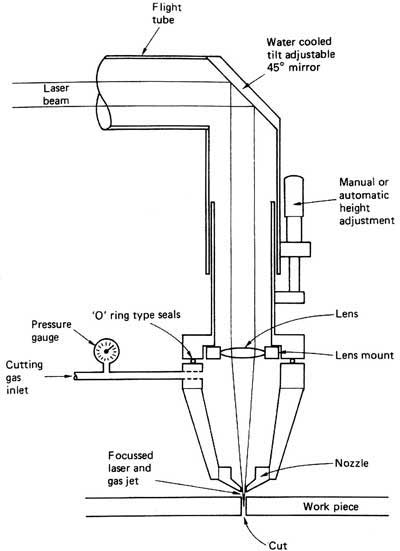
\includegraphics[width=0.6\textwidth]{07_design_for_x/laser-cutter.jpg}
    \caption{Schematic of a laser cutter}\label{fig-cutter}
\end{figure}

Movement is often achieved though either a gantry system where a laser beam is placed perpendicularly to the materials and the beam is directed by three mirrors: one static and two mobile, or a galvanometer system.

\subsubsection{Guidelines}

You\marginnote{Use Material Wisely} will most likely use a full-size sheet for every run you require. So remember to think about how to optimise that use of material. If you know that you will be laser cutting a number of components, try and make them using the same thickness and type of material so that they can be all positioned on the same sheet. This will minimise set-up and change over times. Packing algorithms do exist that optimise positioning of components on two dimensional sheets. The first-fit decreasing height algorithm is one such example.

It\marginnote{Print It Out!} might sound obvious but it's always good to print out your potential laser cut designs so you can check for any issues that might come about through scaling or having selected the wrong units in your CAD software.

The\marginnote{Think about Material Thickness} thicker the material, the longer it will take to cut and cost. It's always good to consider the forces that will be flowing through the part. Smaller thicknesses will speed up prototyping.

Laser\marginnote{Check for Narrow Gaps} cutters typically remove \SI{0.2}{\milli\metre} of material along the line it is tracing (kerf). Therefore, avoid designing parts that have lines with gaps narrower than \SI{1}{\milli\metre} as these will be weak and have a greater chance of breaking.

The\marginnote{Remember the Kerf when Making Assembly Slots} kerf can also effect the fit between your parts. Make sure you take this into consideration when developing your CAD models. You may have a version that fits perfectly on CAD but you may have to create another version of the parts to compensate for the laser cutter.

There\marginnote{Engrave you Group Number and Part Id} will be a lot of parts being laser cut over the summer holidays and you'll have a number of parts that will look similar. Adding an engraving will help identify the parts when you come to build next year.

\subsection{Design for Manufacture (3D Printing)}

3D printing refers to processes in which material is joined or solidified under computer control to create a three-dimensional object. The term is often used interchangeably with Rapid Prototyping and Additive Manufacturing but we tend to use 3D Printing to describe low-cost additive manufacturing systems. And research at the University of Bath has been instrumental in creating low-cost 3D printing.

\begin{marginfigure}
    \centering
    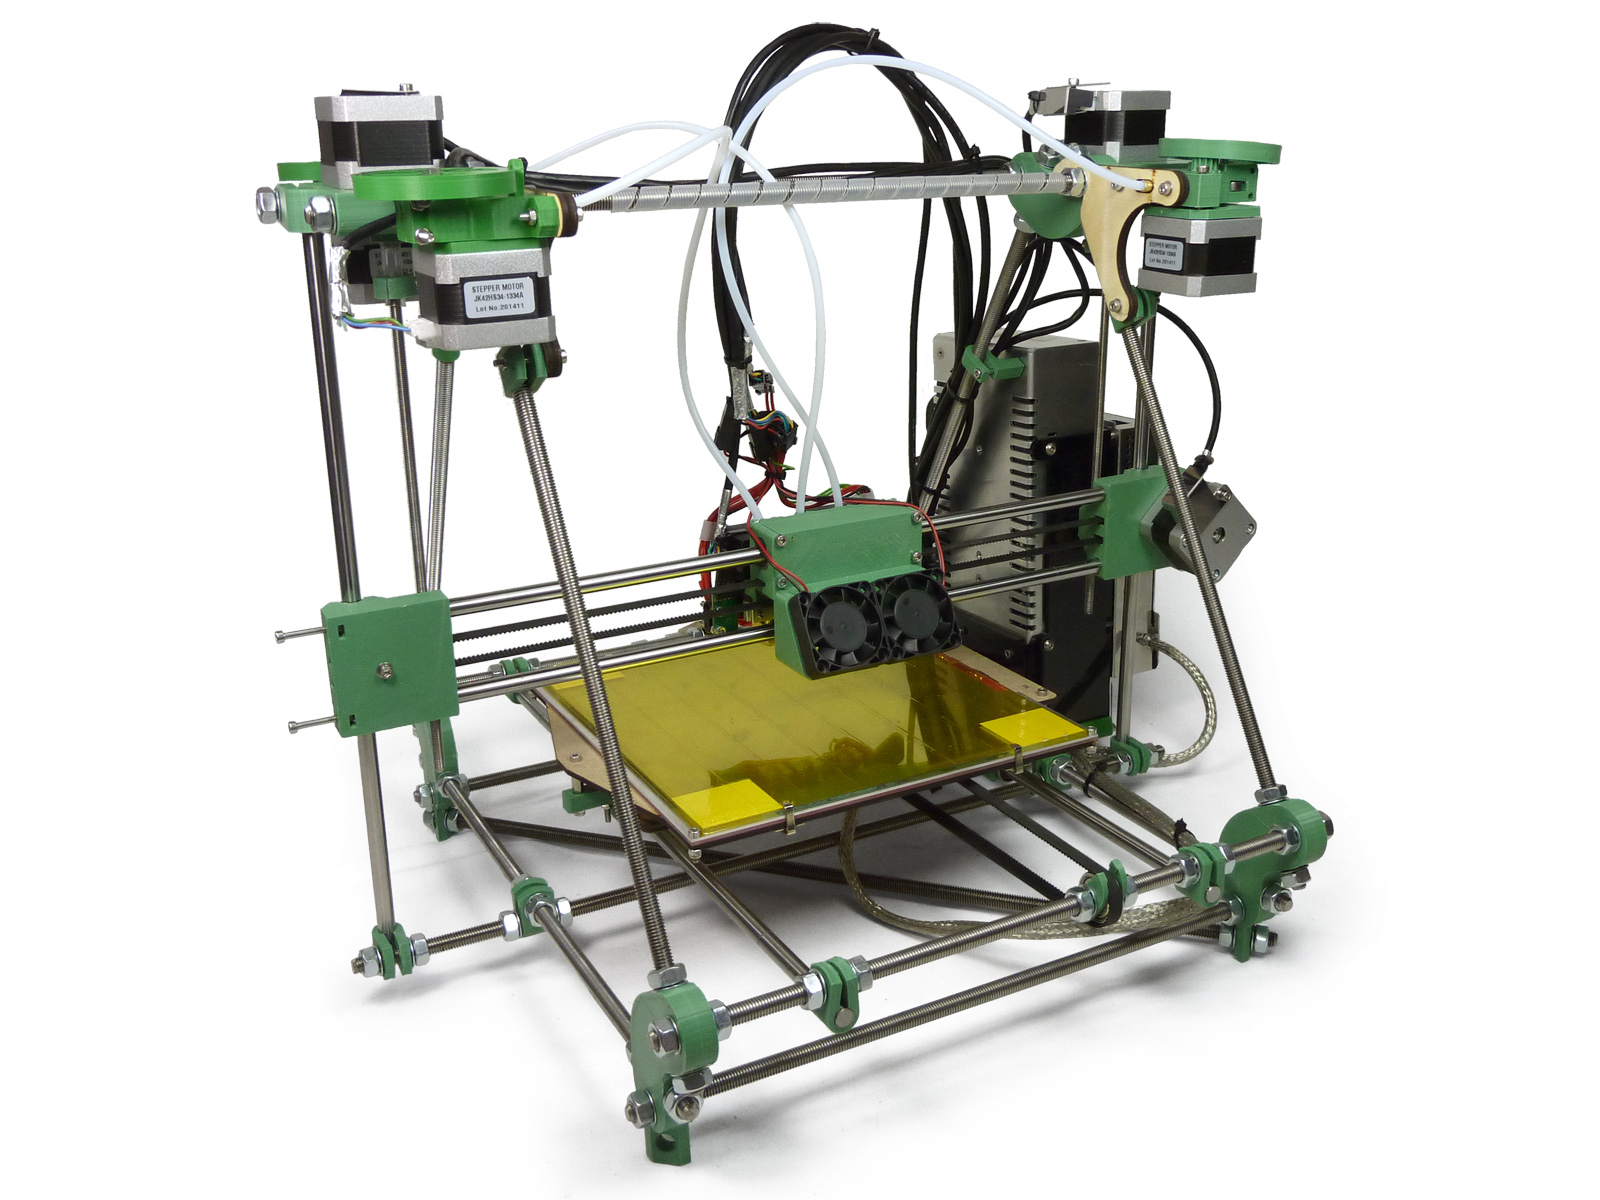
\includegraphics[width=\textwidth]{07_design_for_x/mendel.jpg}
    \caption{Mendel RepRap 3D Printer}
    \label{fig-reprap}
\end{marginfigure}

The work by Dr Bowyer and his colleagues on the open-source RepRap project (\cref{fig-reprap}) has led to the technology that has been implemented in the majority of low-cost Fused Deposition Modelling (FDM) printers on the market today.~\cite{jones2011}

\subsubsection{Types}

There are a number of different types of 3D printing but the most commonly used techniques in rapid prototyping are \acf{FDM} and \acf{SLS}.

\ac{FDM}\marginnote{Fused Deposition Modelling (FDM)}, also known as \acf{FFF} is a 3D printing process that uses a continuous filament of a thermoplastic material. This is fed from a large coil, through a moving, heated extrusion head. The head is \acf{CNC} with the input often being GCode that is turned to machine code to operate the stepper motors on the machine. Extruder temperatures are in the region of \SI{200}{\degreeCelsius}, filament diameters are around \SI{2.85}{\milli\metre} and deposition rates are around \SI{20}{\milli\metre\per\second}.

\ac{SLS}\marginnote{Selective Laser Sintering (SLS)} is a technique that uses a laser to sinter powdered materials. Layers of powdered material is deposited on a bed and after each pass, the laser is directed towards the areas that have been defined in the 3D model as solid geometry. \acf{DMLS} and \acf{SLM} all follow a similar process. The technique was developed and patented by Dr. Deckard in the mid-1980s. The fine-grain structure and accuracy of the laser sintering process enables high-quality prototypes to be generated however, the structural strength of the component is highly-dependent on how well the layers fuse together and there remains is issues when high-tolerances are concerned.

The section now focuses on \ac{FDM} as this is the method that is available to you for your project.

\subsubsection{Terminology}

The\marginnote{Slicing} procedure of taking a \acf{CAD} model and producing the relevant code for the printer to print the model. Users often need to export their \ac{CAD} model as an \acf{STL} file and this is imported into the slicing tool. There are a range of slicing tools that are available and some of the most common are:

\begin{itemize}
    \item Cura
    \item MakerWare
    \item MatterControl
    \item Repetier
    \item Slic3r
\end{itemize}

Research at the University of Bath is leading the development of slicing tools that optimise the internal geometry of printed parts based on the predicted loads through the part \pref{fig-3d-print-bath}~\cite[-3em]{pam2017}.

\begin{figure*}
    
    \hfill
    \subfloat[FEA]{
        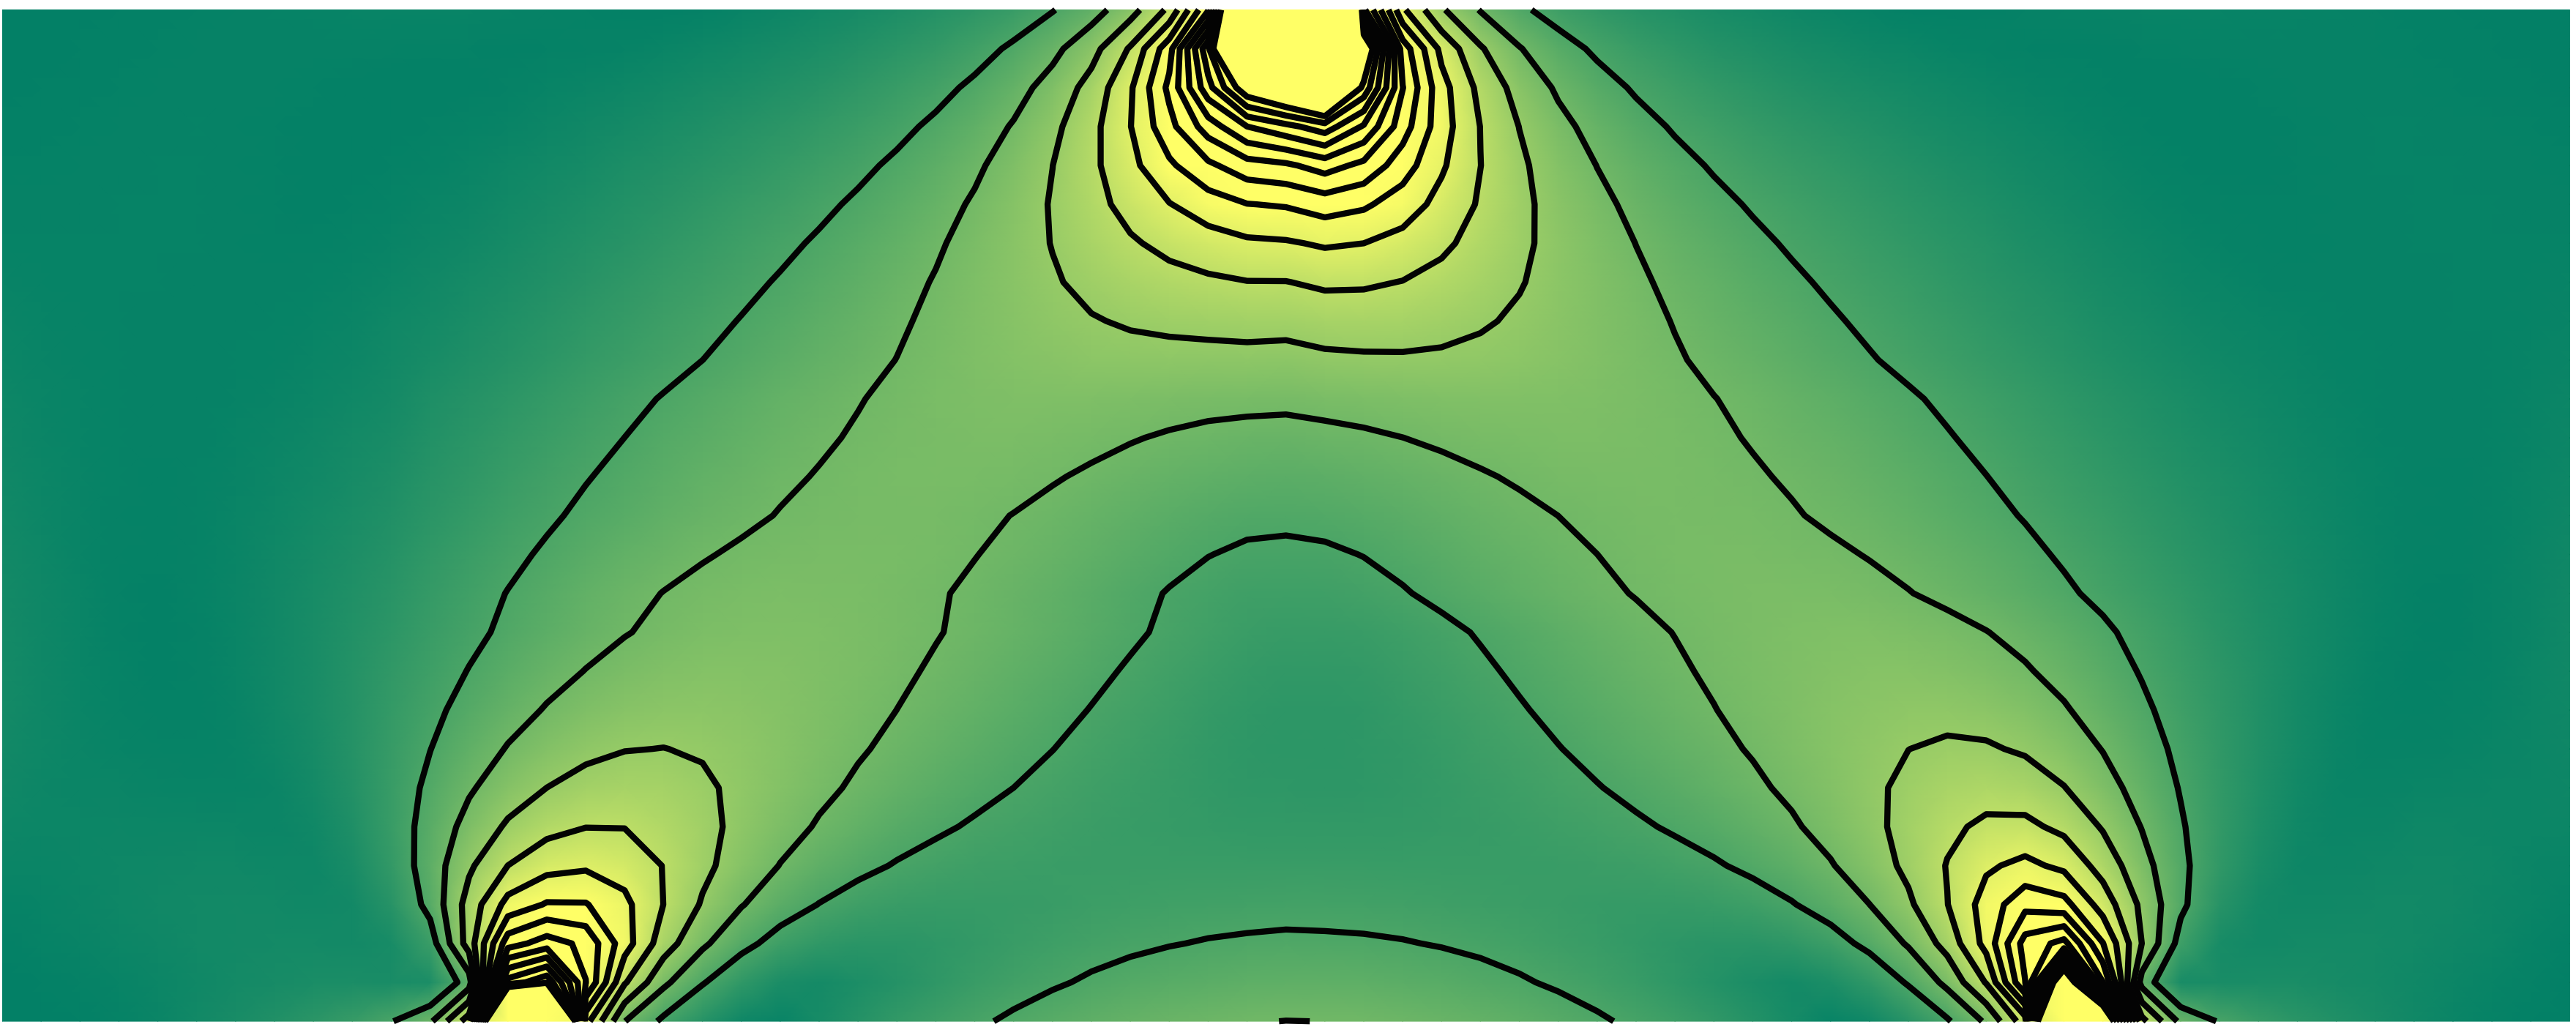
\includegraphics[width=0.45\textwidth]{07_design_for_x/fea_three_point_beam.png}
    }
    \hfill
    \subfloat[Infill Design]{
        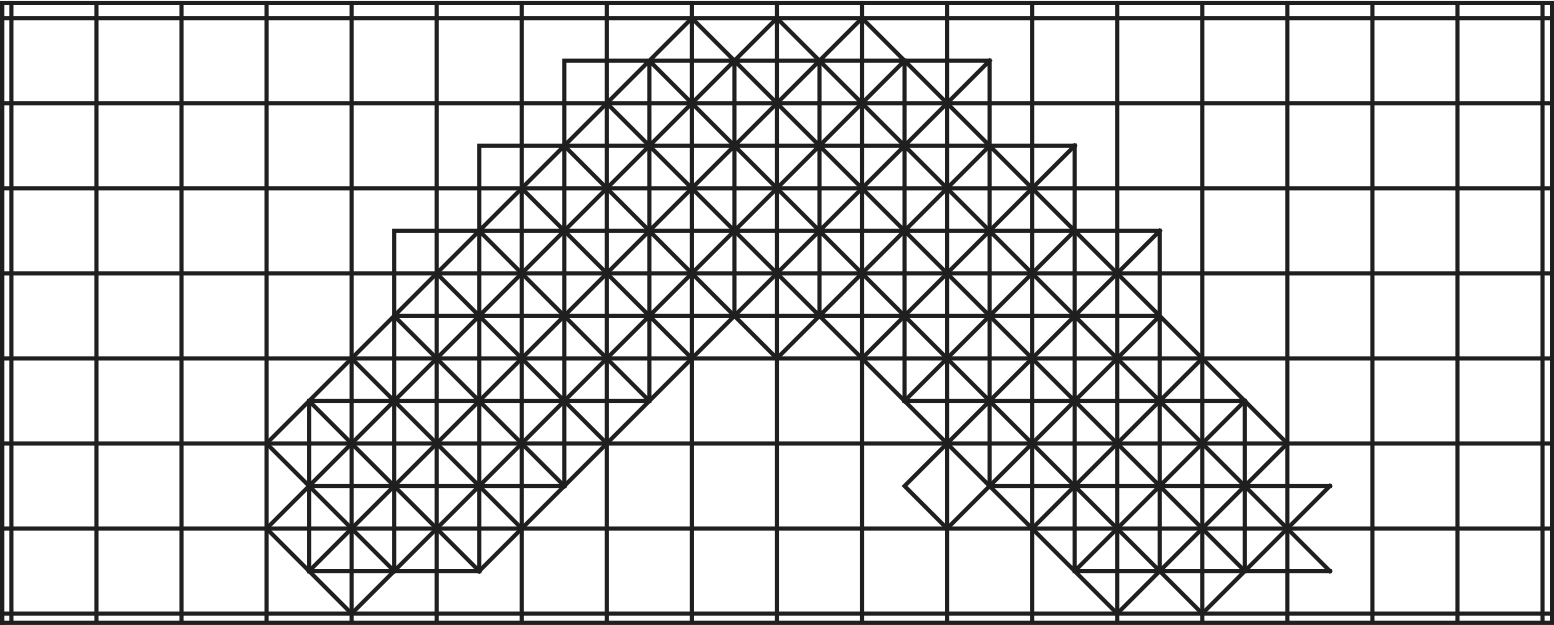
\includegraphics[width=0.45\textwidth]{07_design_for_x/three_point_beam.png}
    }
    \hfill
    
    \vspace{1em}
    \caption{Optimised Lattice Infill for a Three-Point Bend Test}
    \label{fig-3d-print-bath}
\end{figure*}



Slicing tools provide a range of options that aid the user in optimising the print time and material use in creating the prototype. The main options are the number of shells, infill design/density, rafts and supports.

Shells\marginnote[1em]{Shells} are the number of times the 3D printer will print the external geometry of the slice.

Infill\marginnote{Infill} is the design of the internal geometry for the 3D printed part (\cref{fig-infills}). Each infill can have its density adjusted with 100\% being a solid printed part and 0\% being a part within no internal infill. The typical value for infill density is 20\%, which provides a suitable compromise between part strength and print time.

\begin{figure*}[t!]
  \center{}
  \begin{tabular}{p{0.16\textwidth} p{0.16\textwidth} p{0.16\textwidth} p{0.16\textwidth} p{0.16\textwidth}}

  \subfloat[Linear]
  {
  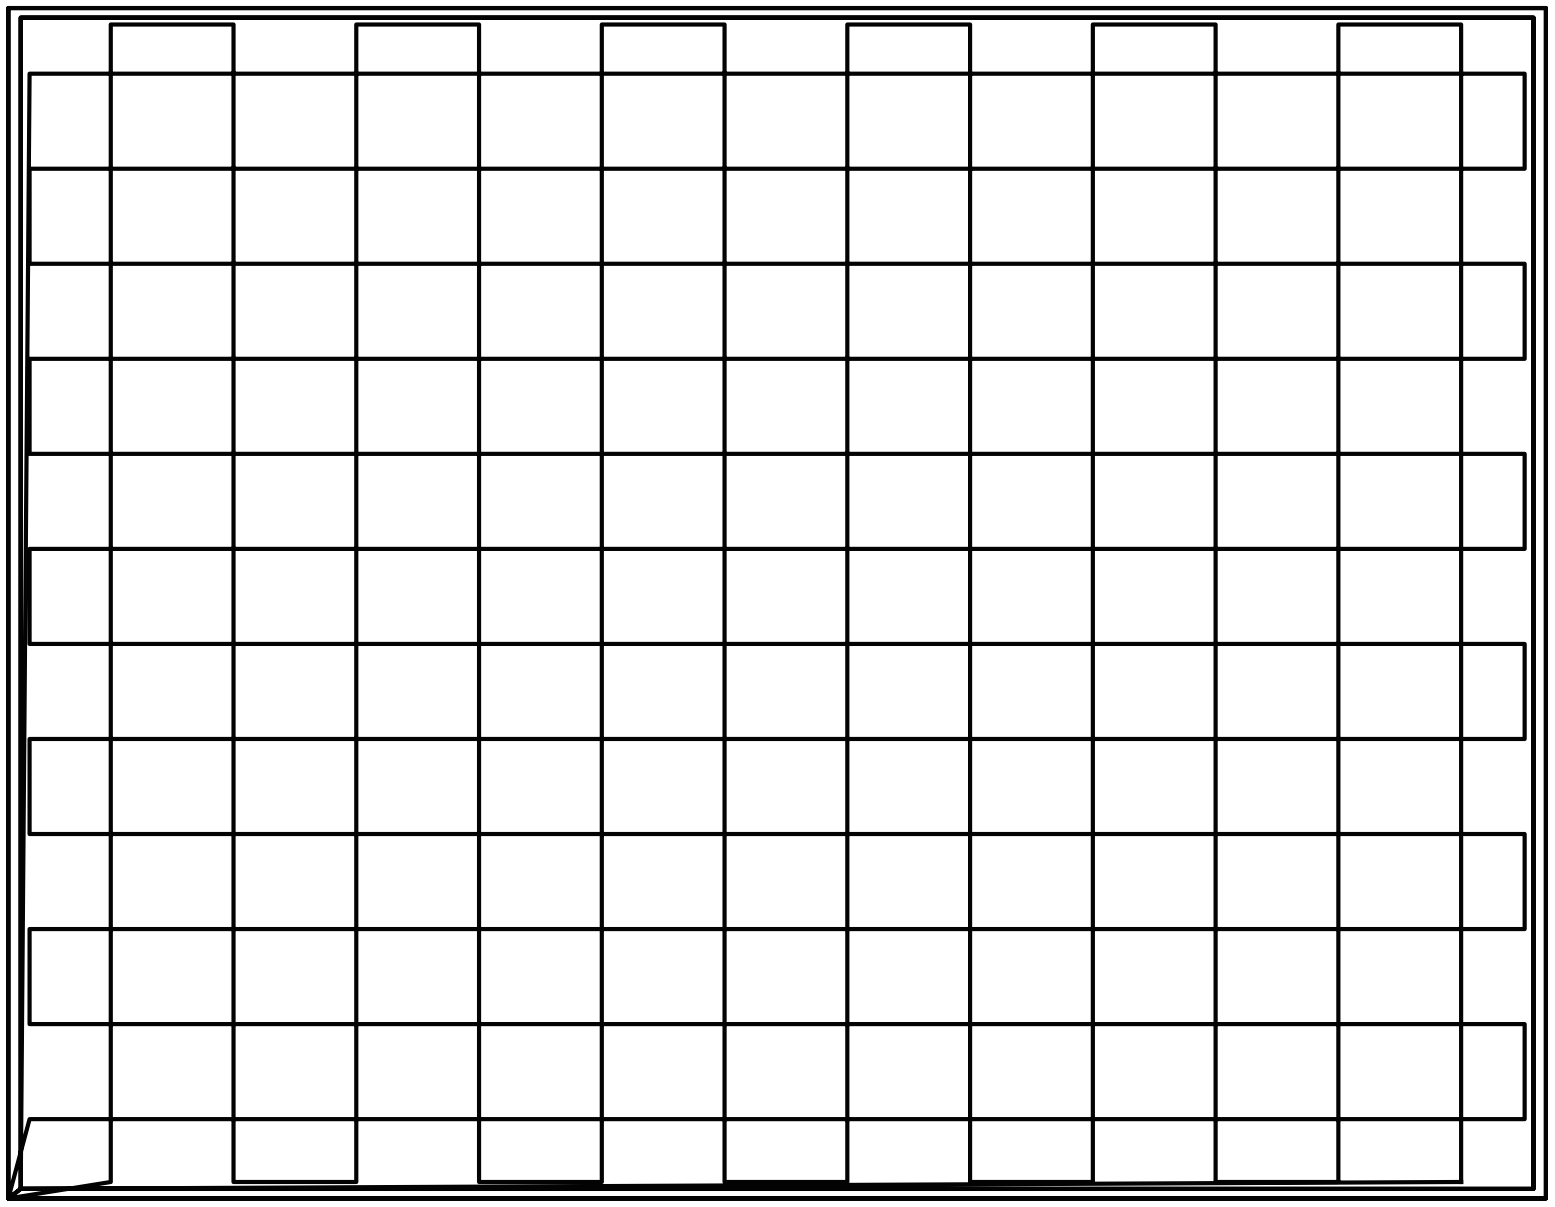
\includegraphics[width=0.18\textwidth]{07_design_for_x/makerbot_infill_strategy_square_linear.png}
  \label{}
  }
  &
  \subfloat[Hexagonal]
  {
  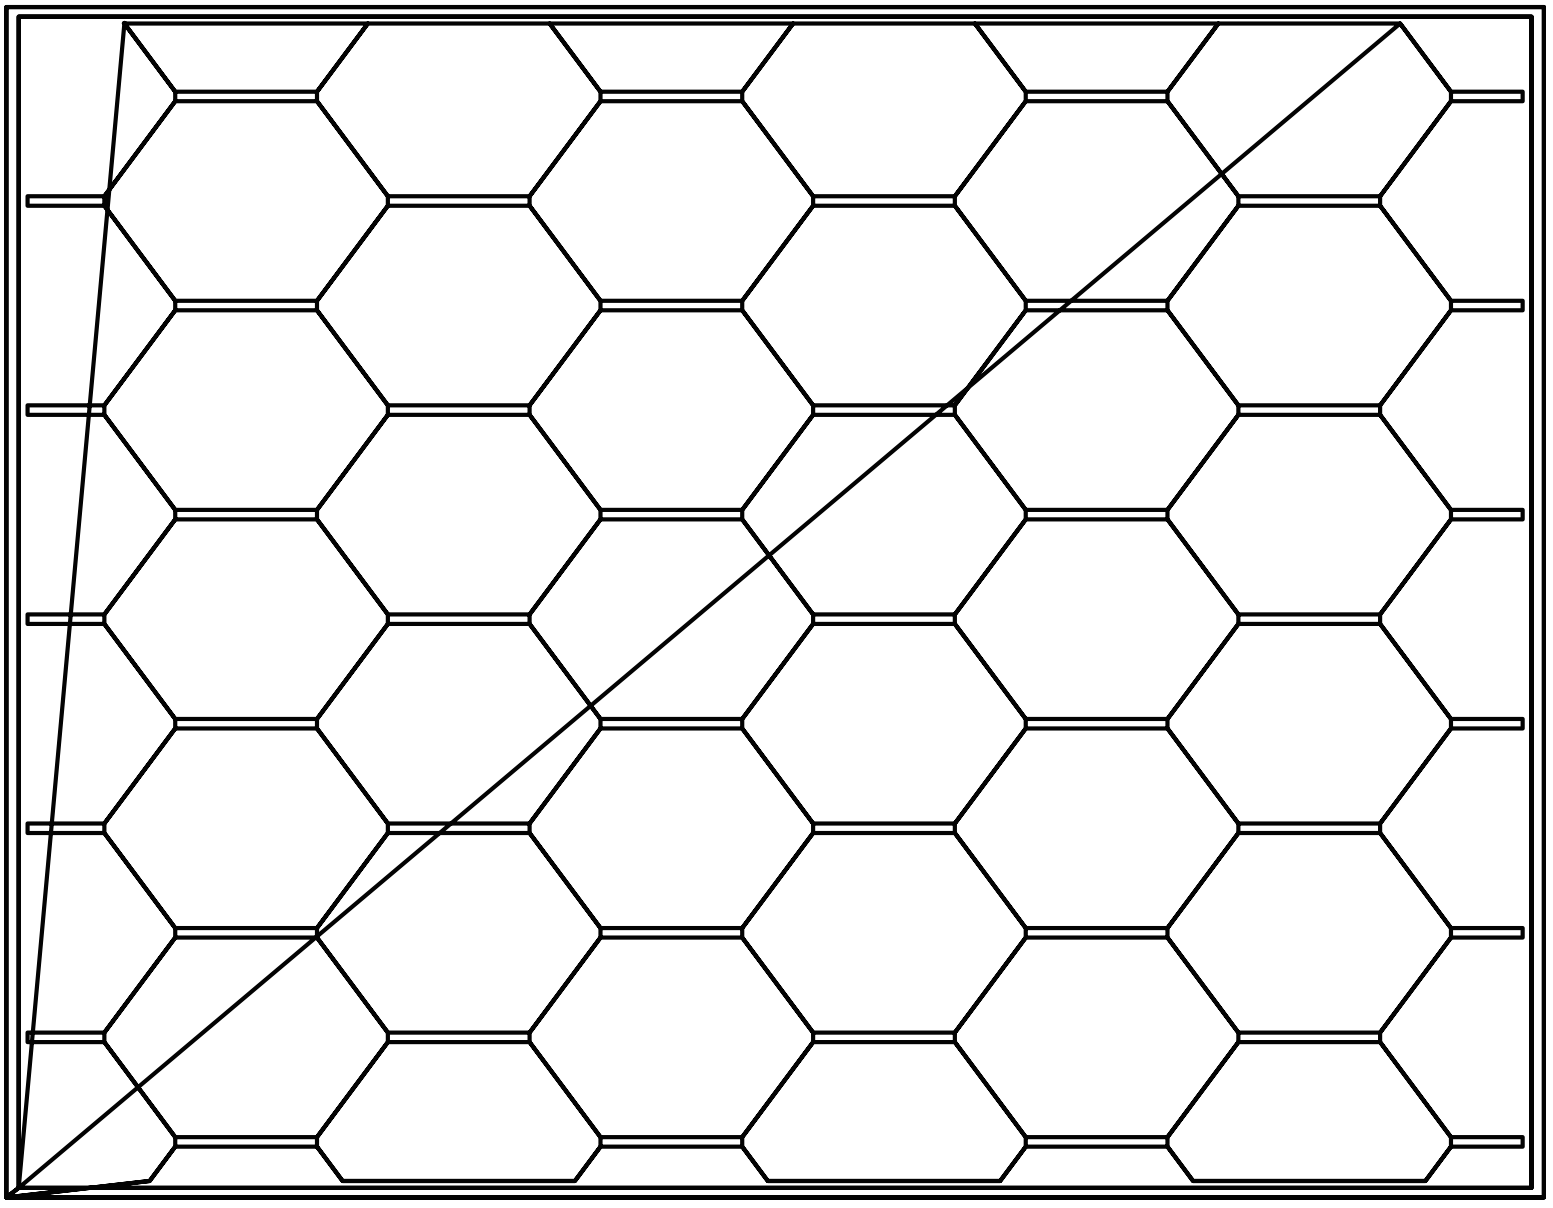
\includegraphics[width=0.18\textwidth]{07_design_for_x/makerbot_infill_strategy_square_hexagonal.png}
  \label{}
  }
  &
  \subfloat[Moroccan Star]
  {
  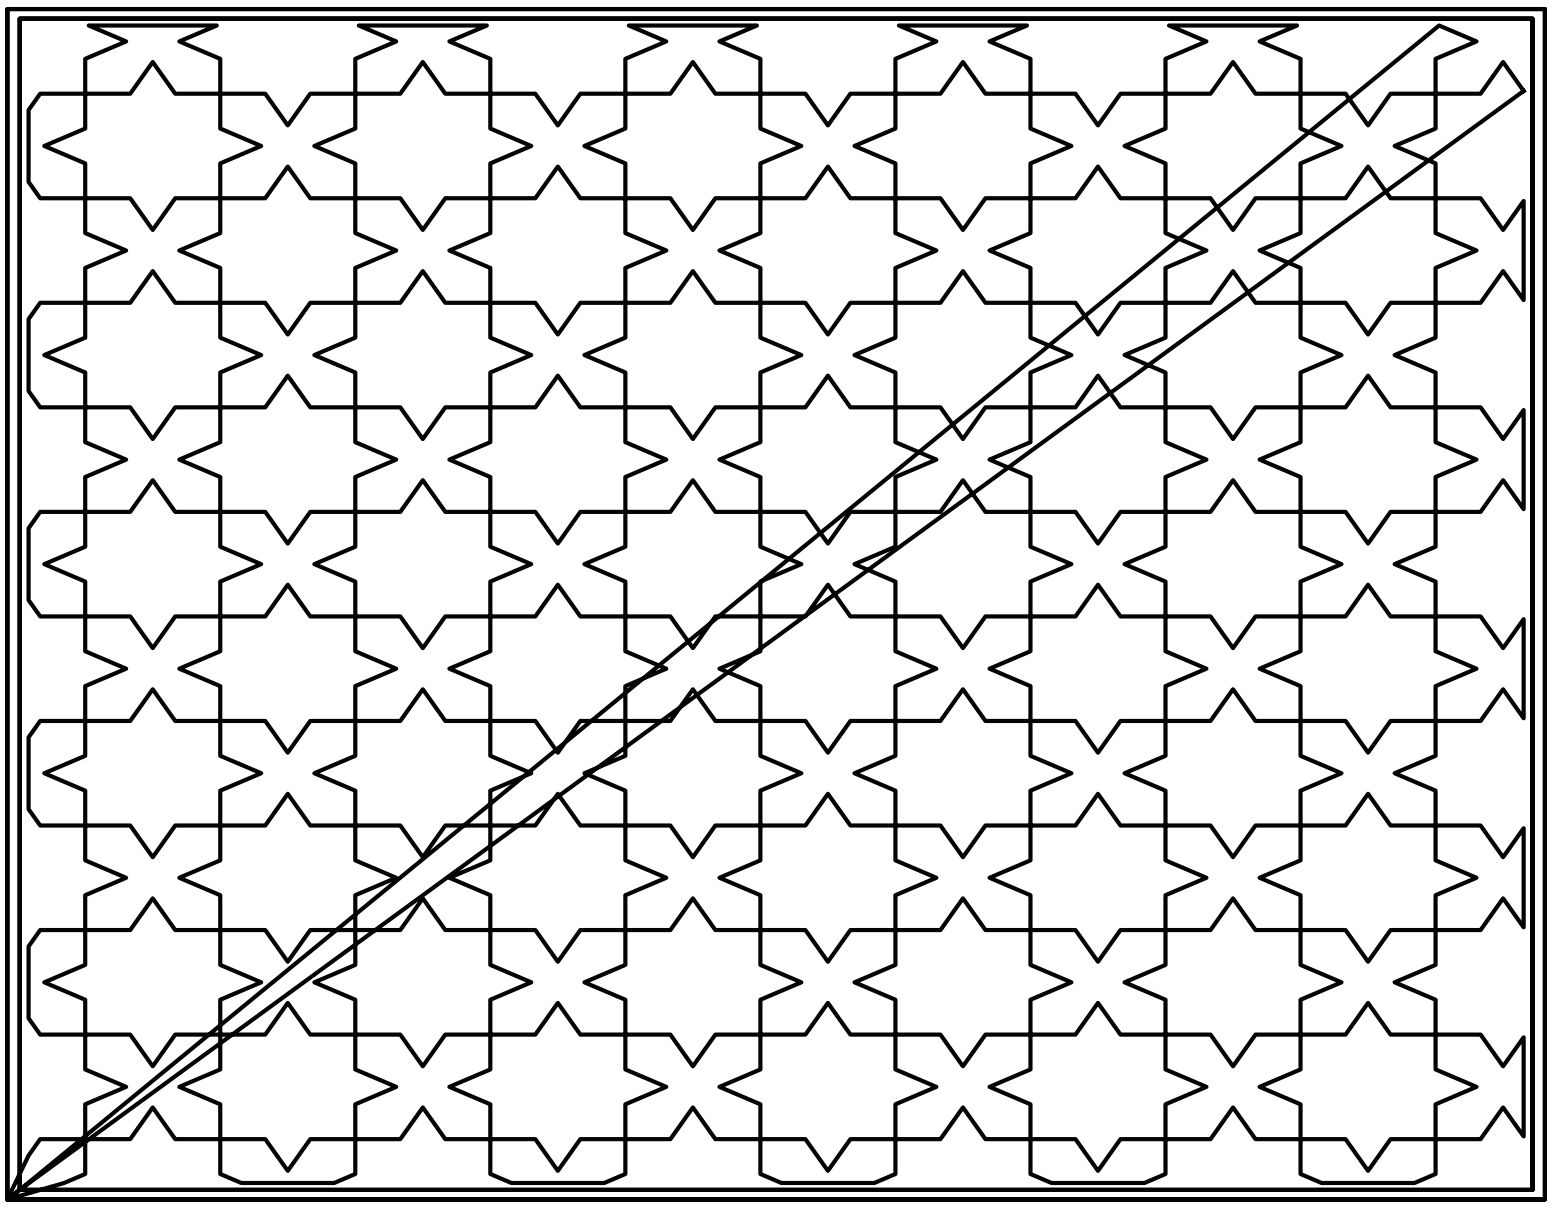
\includegraphics[width=0.18\textwidth]{07_design_for_x/makerbot_infill_strategy_square_moroccanstar.png}
  \label{}
  }
  &
  \subfloat[Catsfill]
  {
  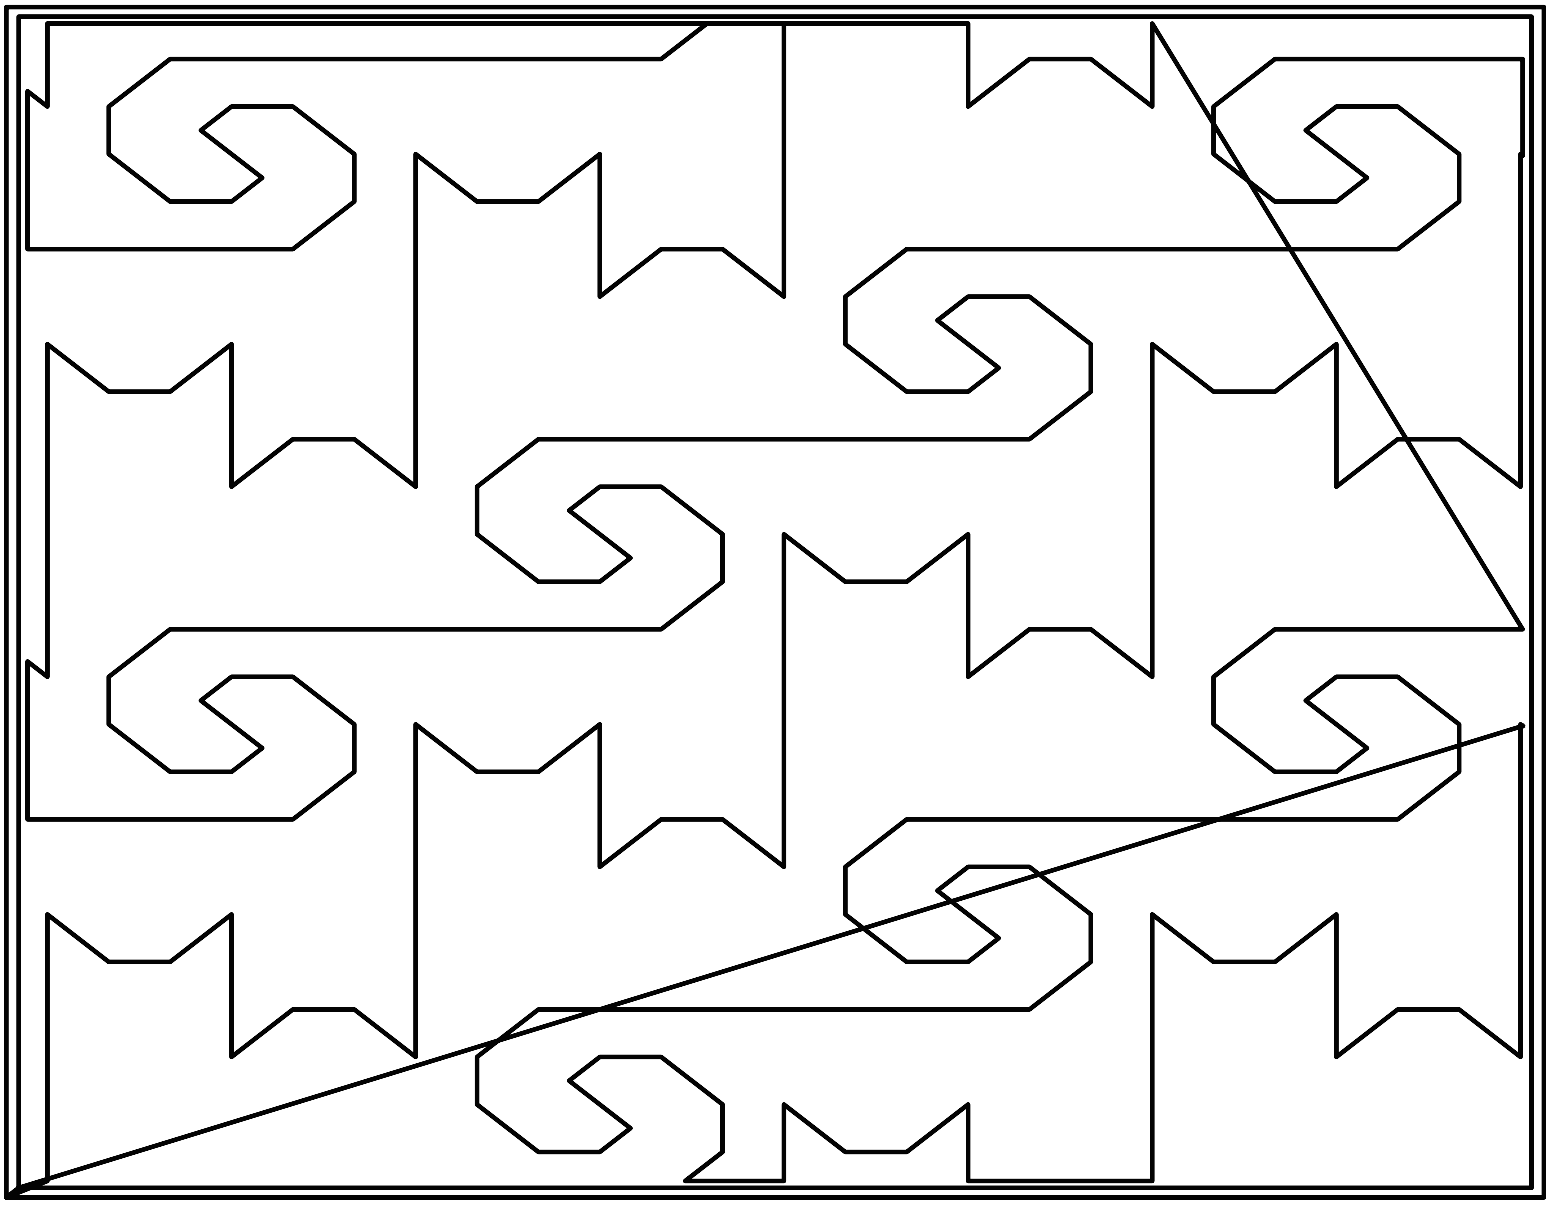
\includegraphics[width=0.18\textwidth]{07_design_for_x/makerbot_infill_strategy_square_catfill.png}
  \label{}
  }
  &
  \subfloat[Sharkfill]
  {
  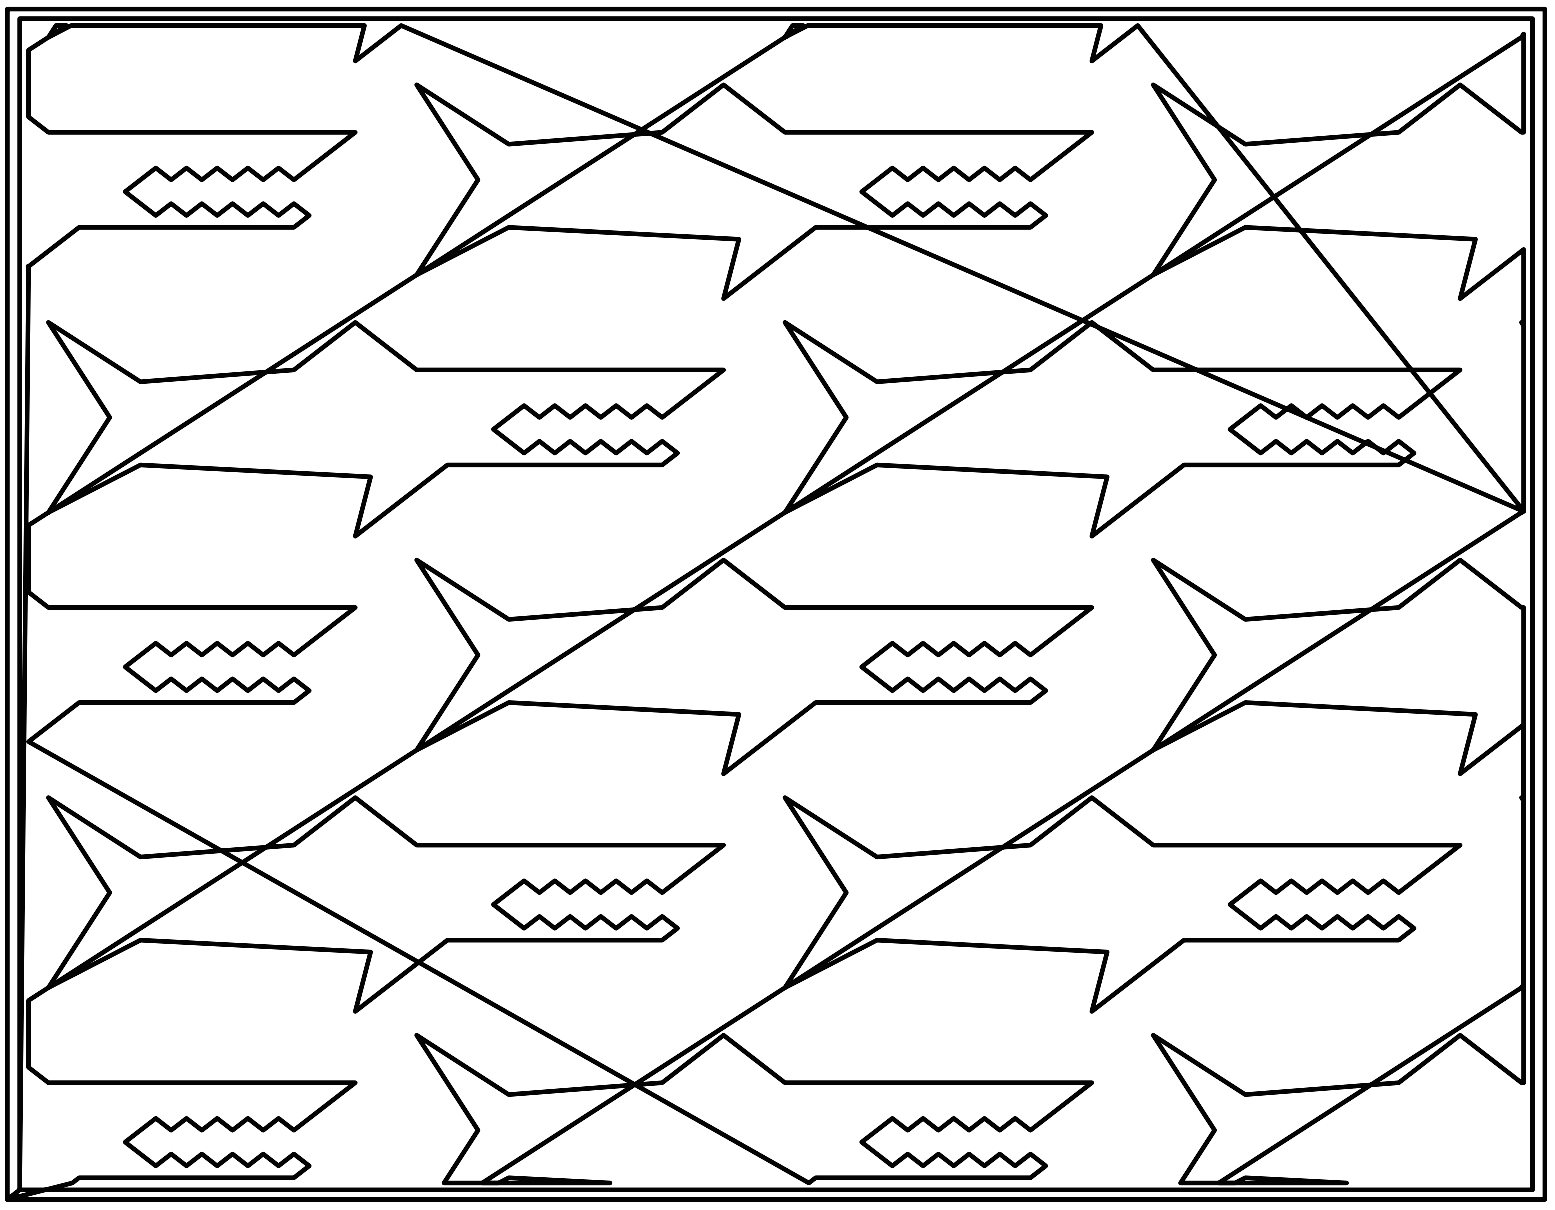
\includegraphics[width=0.18\textwidth]{07_design_for_x/makerbot_infill_strategy_square_sharkfill.png}
  \label{}
  }
  \\

  \subfloat[Line]
  {
  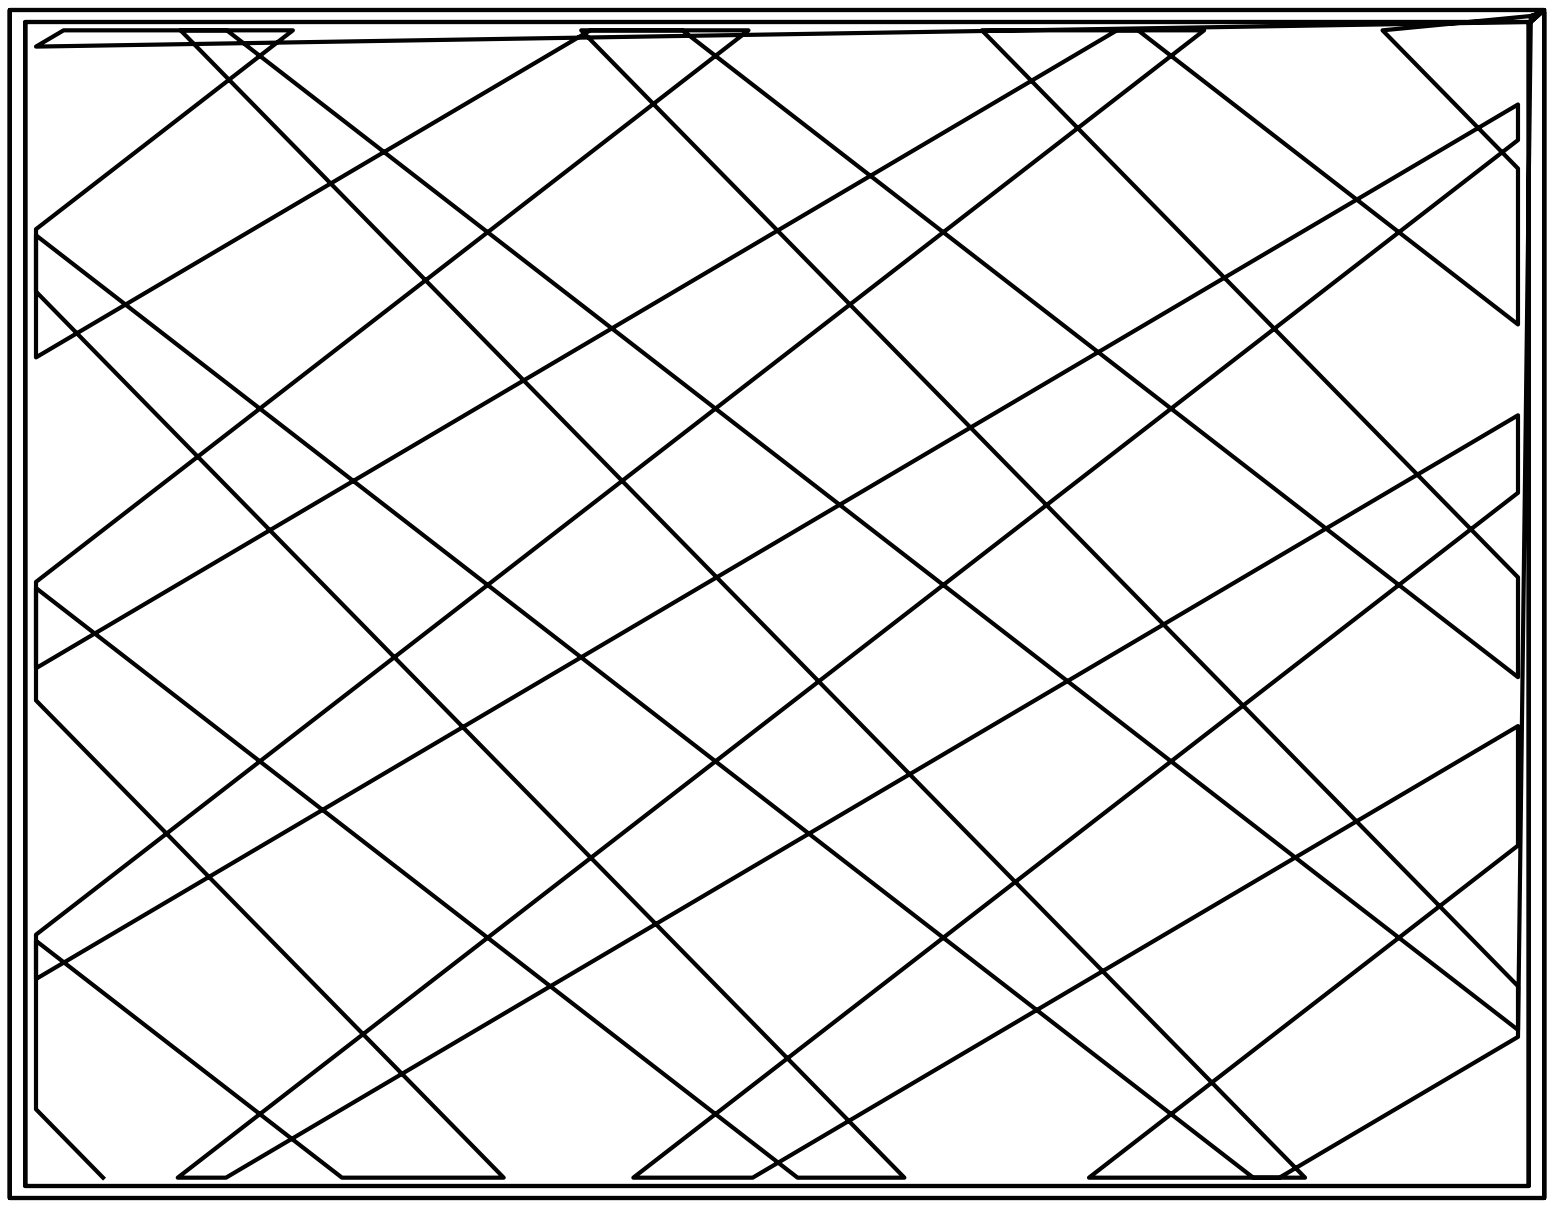
\includegraphics[width=0.18\textwidth]{07_design_for_x/slic3r_plate_line.png}
  \label{}
  }
  &
  \subfloat[Rectilinear]
  {
  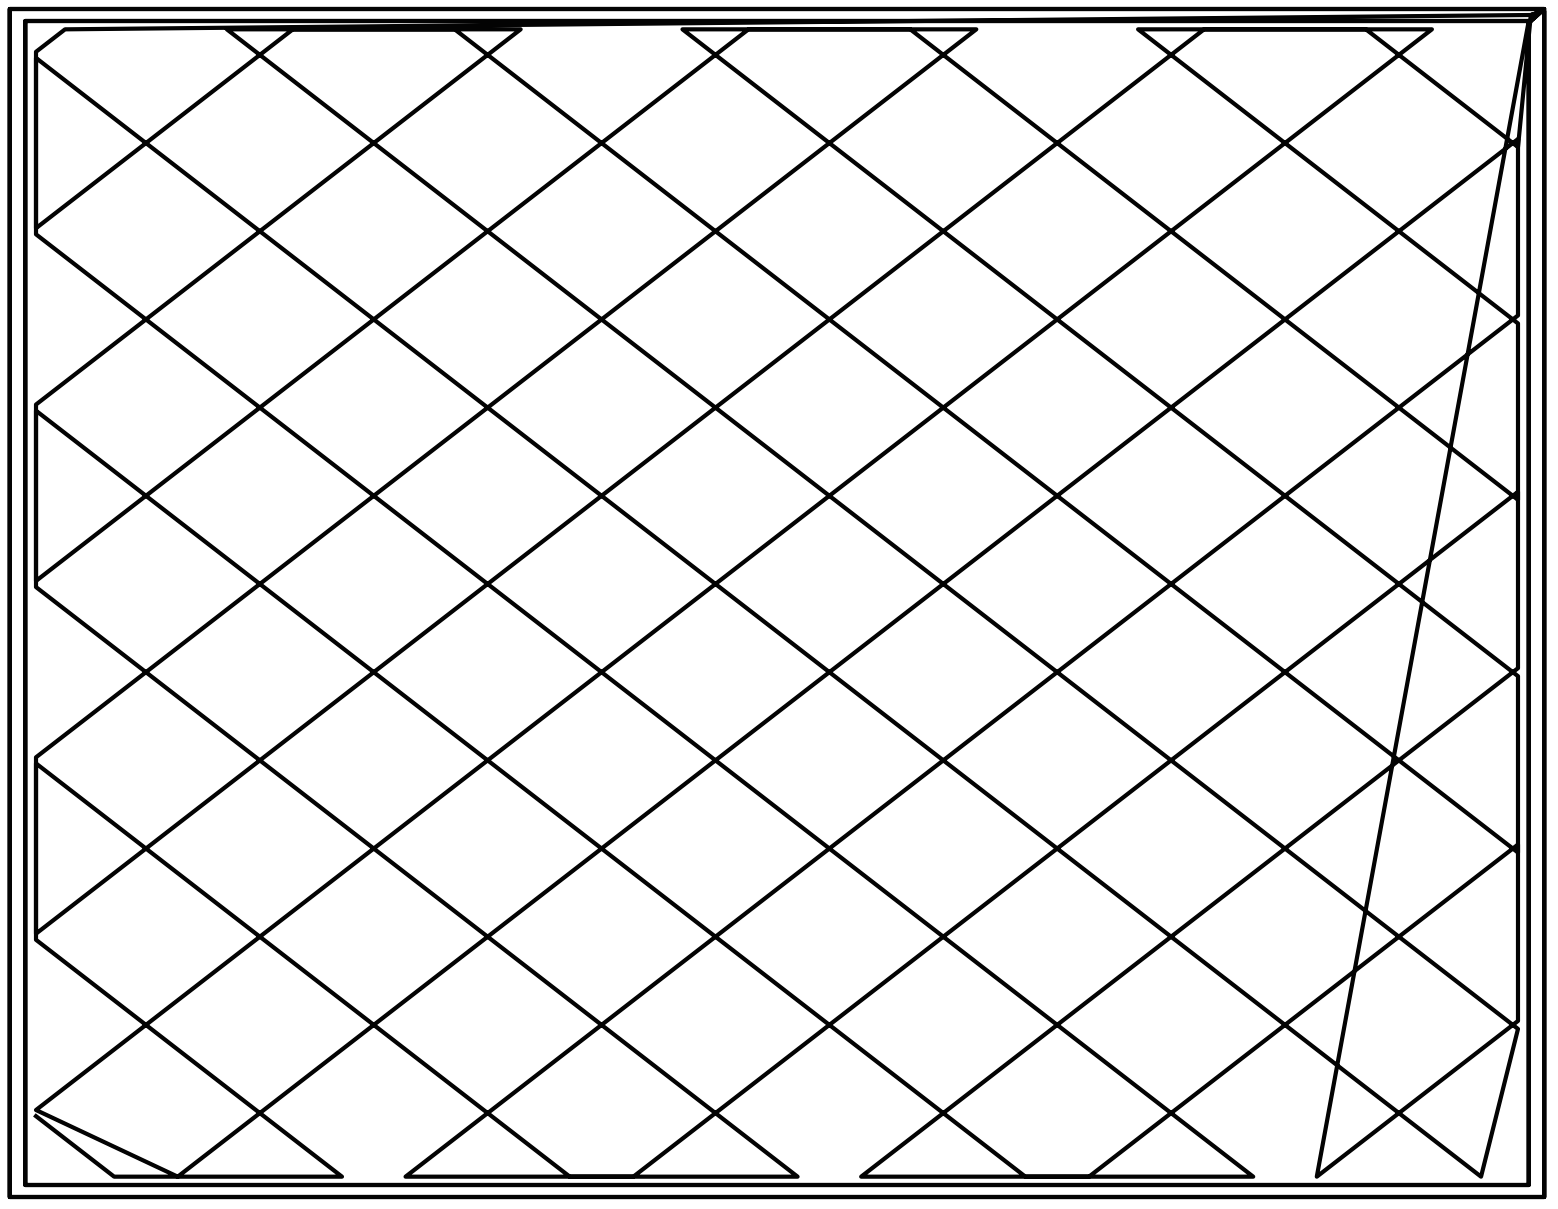
\includegraphics[width=0.18\textwidth]{07_design_for_x/slic3r_plate_rectilinear.png}
  \label{}
  }
  &
  \subfloat[Concentric]
  {
  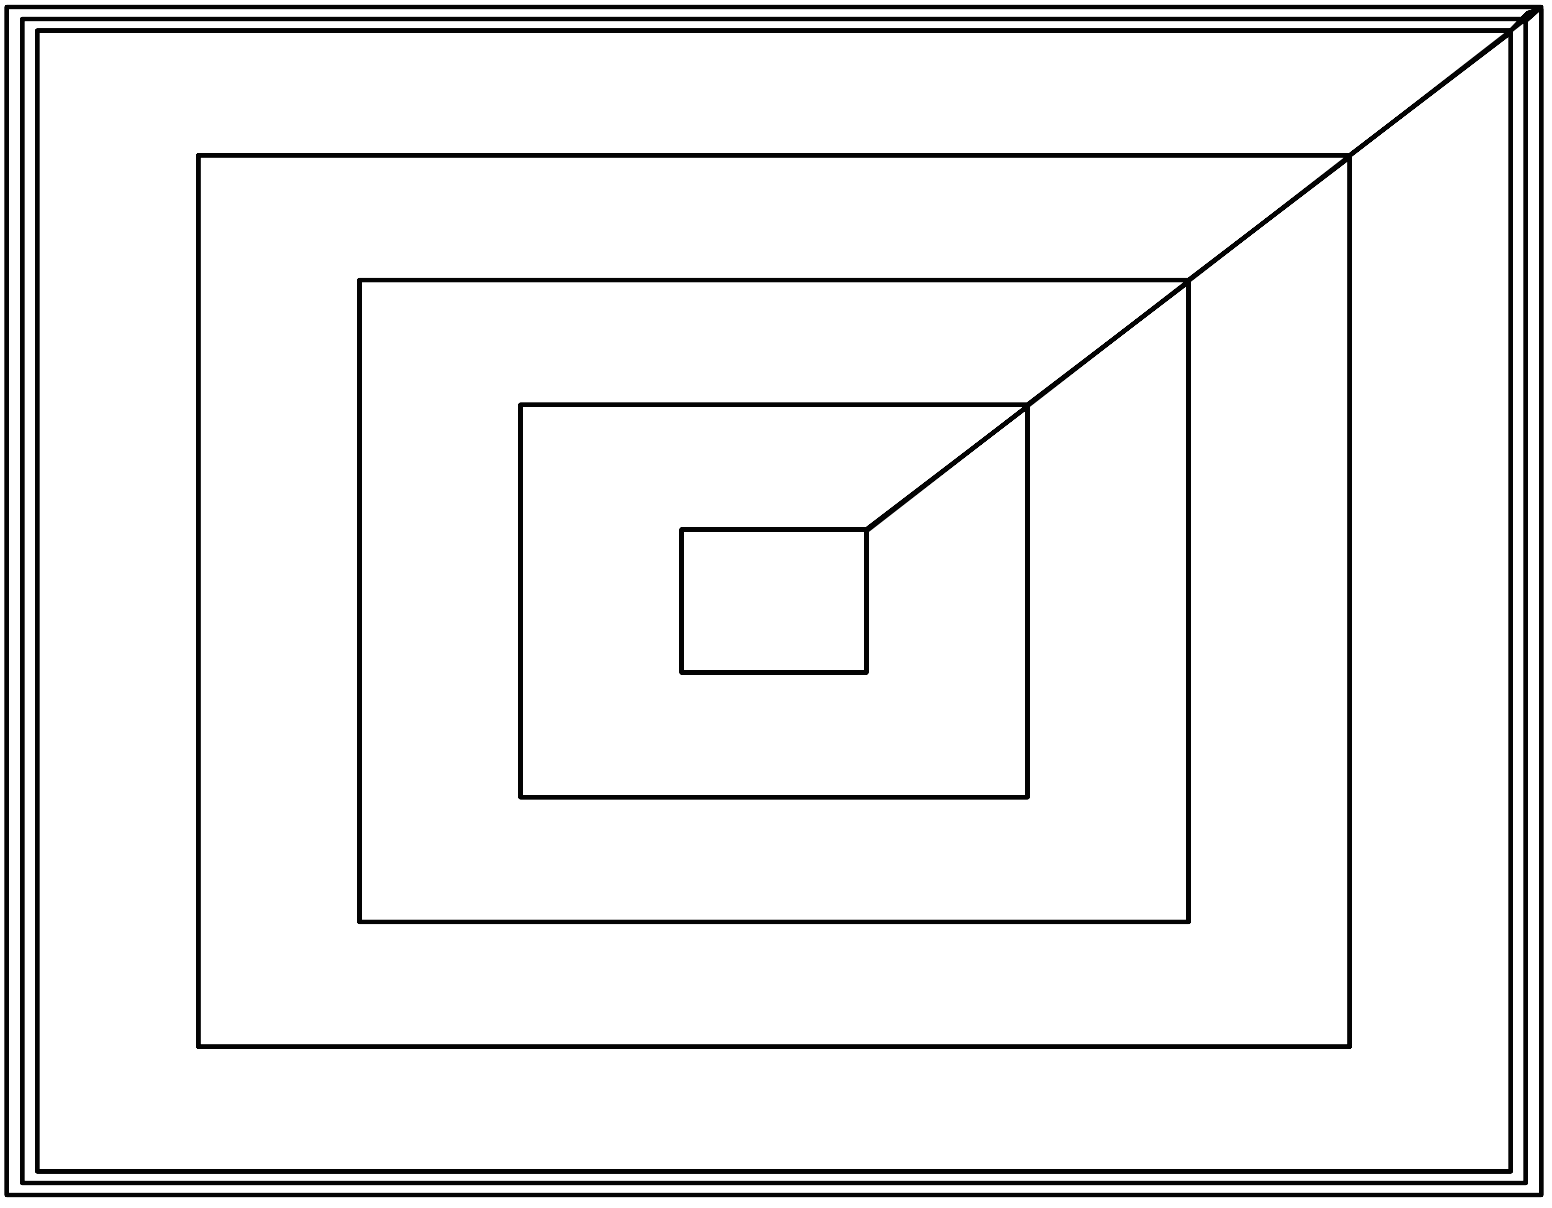
\includegraphics[width=0.18\textwidth]{07_design_for_x/slic3r_plate_concentric.png}
  \label{}
  }
  &
  \subfloat[Hilbert Curve]
  {
  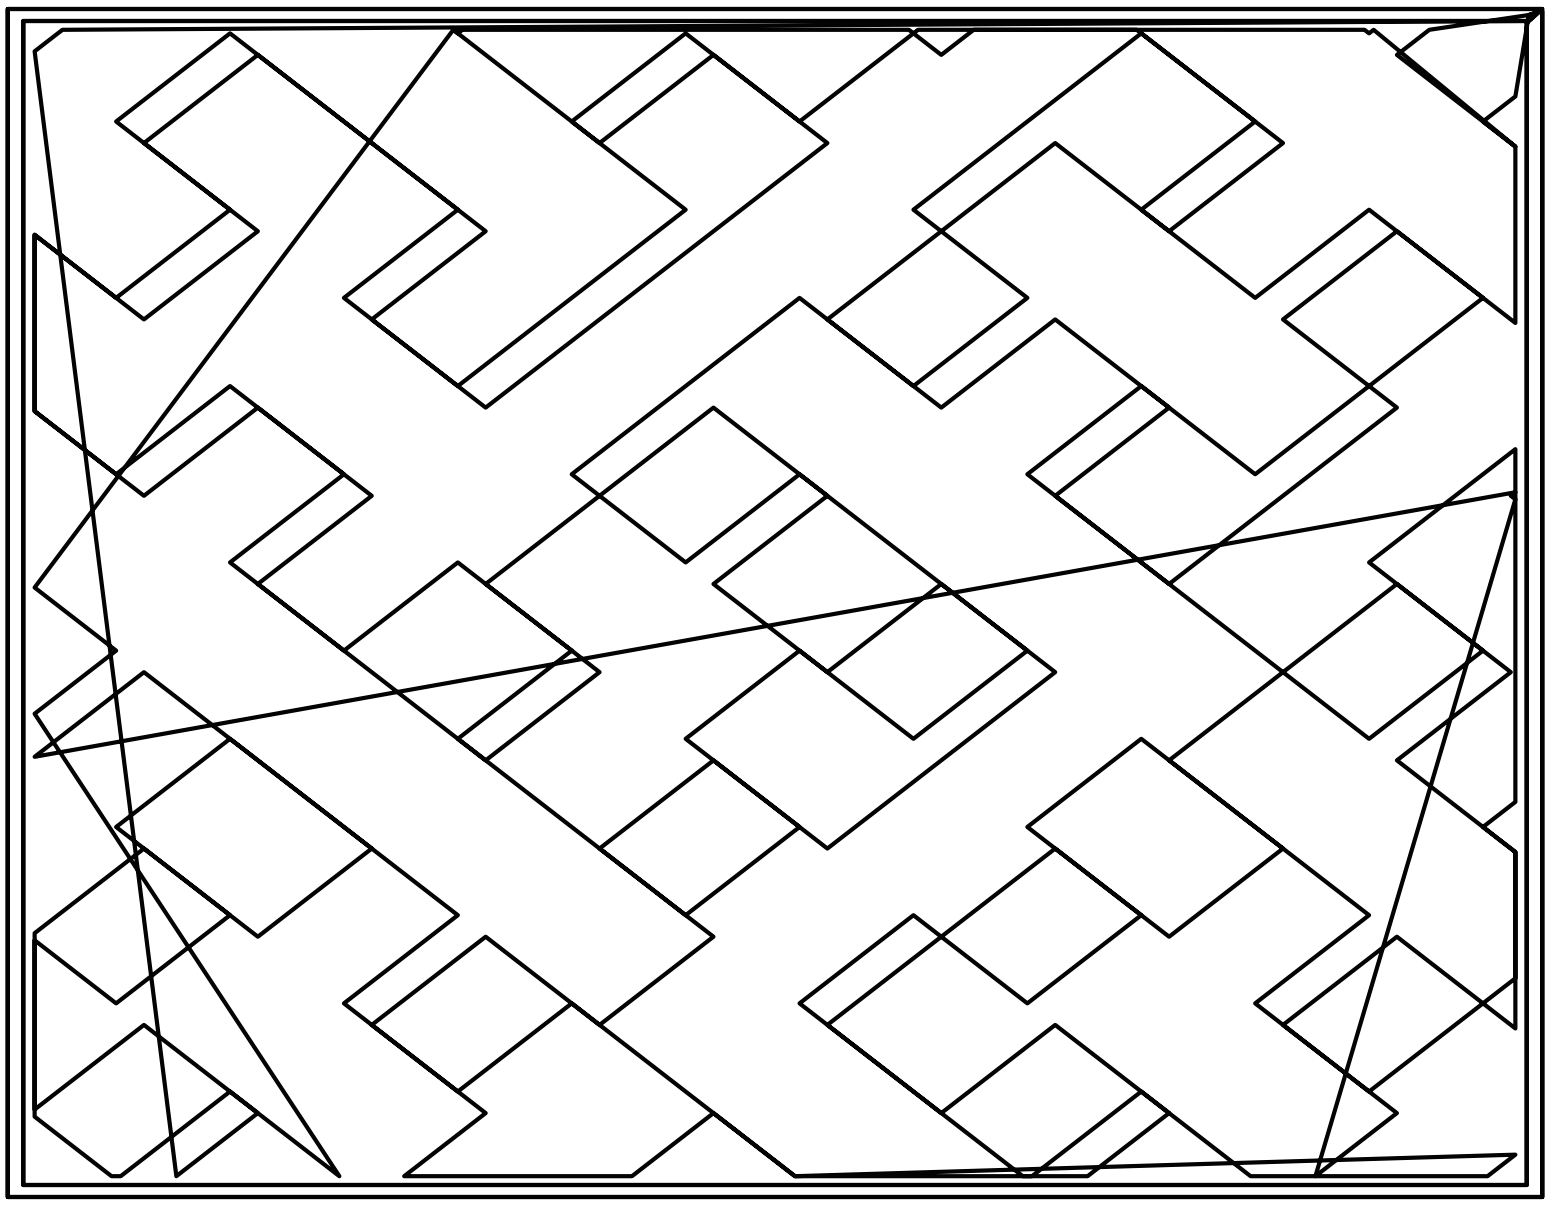
\includegraphics[width=0.18\textwidth]{07_design_for_x/slic3r_plate_hilbertcurve.png}
  \label{}
  }
  &
  \subfloat[Archimedean Chords]
  {
  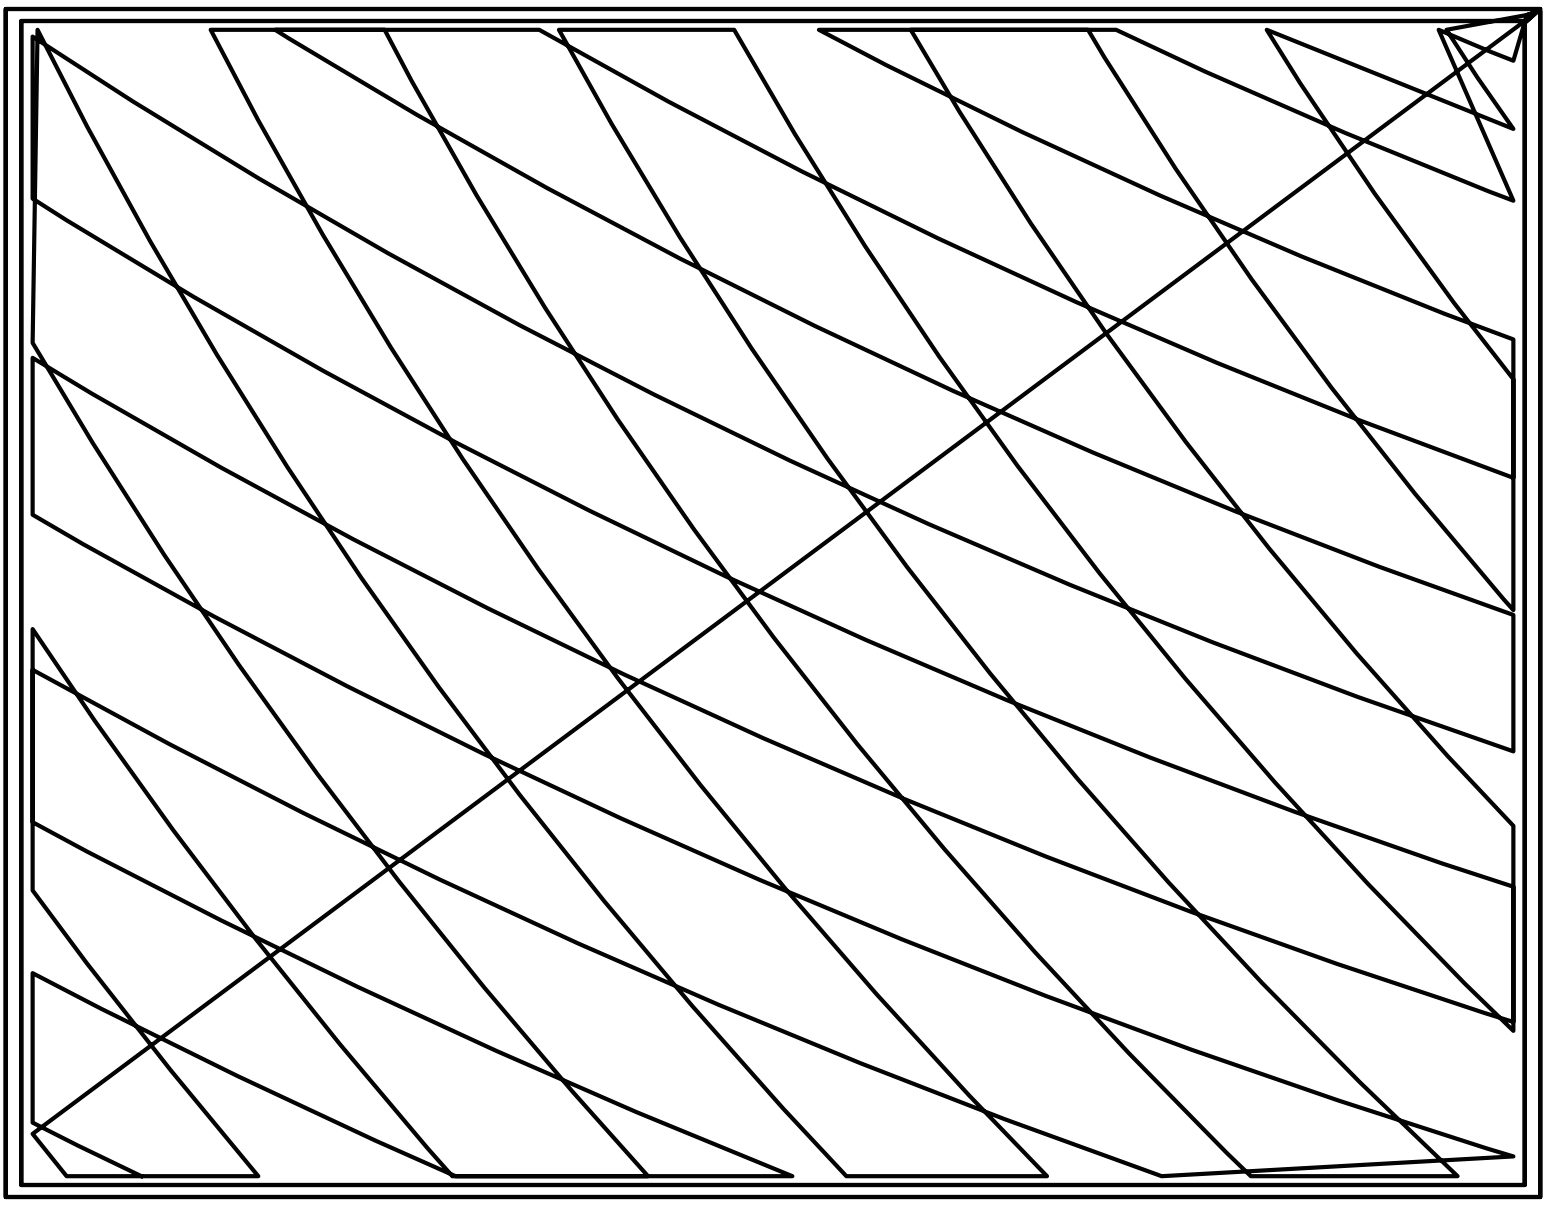
\includegraphics[width=0.18\textwidth]{07_design_for_x/slic3r_plate_archimedeanchords.png}
  \label{}
  }
  \\

  \end{tabular}
  \vspace{1em}
  \caption{Infill Strategies from MakerWare (a-e) \& Slic3r (f-j) Software}
\label{fig-infills}
\end{figure*}

Rafts\marginnote{Rafts} are printed onto the print bed ahead of the part being printed. This provides an adhesive layer for the part to be printed on and reduces the chance of the print warping and/or separation from the print bed occurring.

Supports\marginnote{Supports} can be selected to help with parts that contain overhangs or features that require bridging. This enables more complex geometries to be produced but at the cost of additional post-processing and finishing of parts.

The level of support can be reduced considerably if you try different orientations of a part on the print bed. In addition, new multi-head printers allow for the printing of soluble support material, which can be dissolved by placing the printed part in water.

Layer height\marginnote[-2em]{Layer Height} is typically measured in \si{\milli\metre}. The larger the height, the quicker the print and coarser the finish. It is often best to leave this parameter at its default setting. Although, there is research looking into adaptive layer heights where the slicing tool will automatically reduce the layer height when the slicer identifies complex areas of geometry.\cite[-6em]{pandey2003}\cite[-1em]{sabourin1996}

The\marginnote{G-Code} language used to communicate motor movements and deposition of the filament.


\subsubsection{Slicing Process} 

Slicing is the process of generating the GCode for a 3D Model. In this section, we will go through the process of slicing a simple rectangular block where we do not have to consider the addition of rafts and supports. Although you will be using a slicing program to automatically do this, it is good to know what is going one behind the scenes. You never know when you may want to generate your own custom GCode for a 3D printer to use. The main steps are:

\begin{enumerate}
    \item Identifying the perimeter geometry
    \item Creating shells
    \item Creating the internal linear mesh
    \item Determining the printer travel path
    \item Creating the GCode printer file
\end{enumerate}

\begin{figure}[h!]
    \centering
    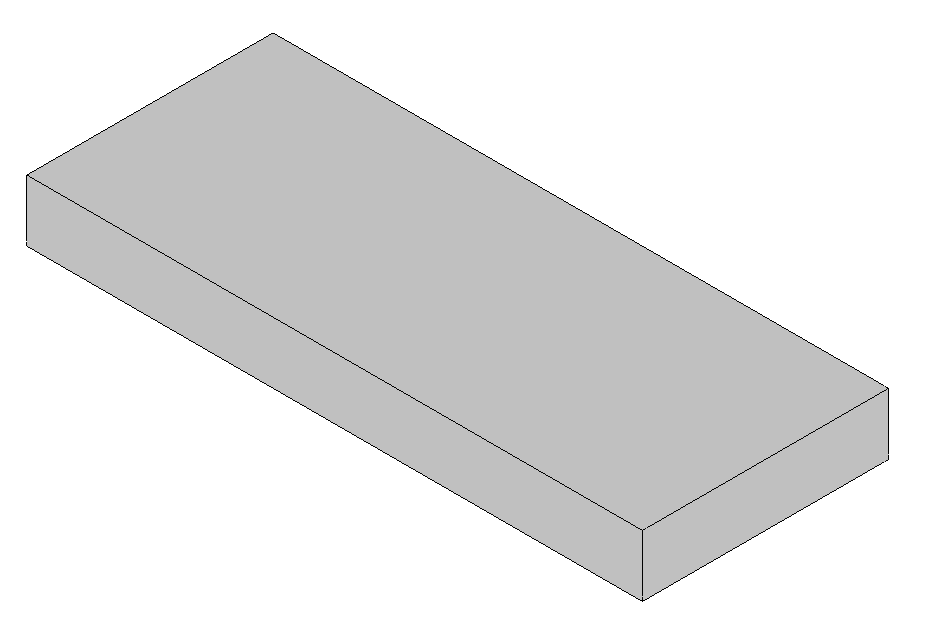
\includegraphics[width=0.7\textwidth]{07_design_for_x/beam_stl.png}
    \caption{Rectangular block to be sliced}\label{fig-block}
\end{figure}


We\marginnote{Perimeter Identification} will now go through the procedure for one slice of the rectangular block (\cref{fig-block}). The first step is to identify for the perimeter on the plane at which we wish to slice. To achieve this, a slicing plane is generated and the intersections between the plane and the \ac{STL} model are identified \pref{fig-intersection}.
A set of lines is then generated from where the plane intersects the individual polygons of the \ac{STL} file. It is then the case of identifying the connecting path between the lines. This is achieved by taking a single line and identifying the neighbouring line by finding the end points that match. The process then continues to the end of the next line and repeats until the sequences of lines returns to the starting line. This forms a perimeter polygon for the part. There is then a check to see whether any lines remain that do not form part of the chain. If so, a new chain is generated with the remaining lines. This cycle repeats until all the lines are associated to a chain. This enables the identification of complex geometry with multiple perimeters such as a part containing holes and/or cut-outs.

\begin{figure}[h!]
  \center
  \tdplotsetmaincoords{45}{135}
  \begin{tikzpicture}[scale=0.5, tdplot_main_coords]
    \coordinate (O) at (0,0,0);
    \draw[thick] (0, 0, 0) -- (0, 10, 0) -- (4, 10, 0) -- (4, 0, 0) -- (0, 0, 0);
    \draw[thick] (0, 0, 2) -- (0, 10, 2) -- (4, 10, 2) -- (4, 0, 2) -- (0, 0, 2);

    \draw[thick] (0,0,0) -- (0,0,2);
    \draw[thick] (0,10,0) -- (0,10,2);
    \draw[thick] (4,10,0) -- (4,10,2);
    \draw[thick] (4,0,0) -- (4,0,2);

    \draw[fill=gray, fill opacity=0.2] (-0.5, -0.5, 0.6) -- (-0.5, 10.5, 0.6) -- (4.5, 10.5, 0.6) -- (4.5, -0.5, 0.6) -- (-0.5, -0.5, 0.6);
    \draw[dashed] (0, 0, 0.6) -- (0, 10, 0.6) -- (4, 10, 0.6) -- (4, 0, 0.6) -- (0, 0, 0.6);

    \draw[->] (7,5,0) -- (7,6,0) node[right]{x};
    \draw[->] (7,5,0) -- (6,5,0) node[right]{y};
    \draw[->] (7,5,0) -- (7,5,1) node[anchor=south]{z};

  \end{tikzpicture}
  \caption{Cutting planes through the beam STL}
  \label{fig-intersection}
\end{figure}


With\marginnote{Shells} the perimeter identified, one can perform a transform on the perimeter polygon that has an offset applied to create a duplicate perimeter within a filament width of the previous polygon. The number of times this is performed is determined by the number of shells you wish to have for your model.


\begin{figure}[h!]
  \centering
    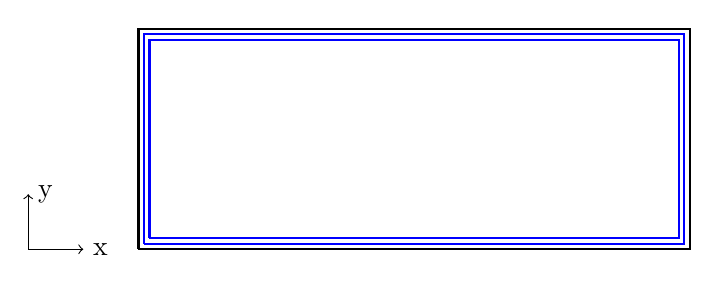
\begin{tikzpicture}[scale=0.7]
      \draw[thick] (0,0) -- (10,0) -- (10,4) -- (0,4) -- (0,0);
      \draw[thick, blue] (0.1,0.1) -- (9.9,0.1) -- (9.9,3.9) -- (0.1,3.9) -- (0.1,0.1);
      \draw[thick, blue] (0.2,0.2) -- (9.8,0.2) -- (9.8,3.8) -- (0.2,3.8) -- (0.2,0.2);
      \draw[->] (-2,0) -- (-1,0) node[right]{x};
      \draw[->] (-2,0) -- (-2,1) node[right]{y};
    \end{tikzpicture}
    \caption{Creating shells from the perimeter polygon}\label{fig-shells}
\end{figure}

The\marginnote{Linear Mesh Generation} third step of the process involves the generation of a set of uniformly distributed vertical and horizontal lines to form the linear infill design for the part. The linear infill width sizing is derived from the infill density perimeter that is set in the software. The process then generates rays along the x \& y axes for the given layer height, and identifies the intersections of rays against the \ac{STL} model of the part (Figures~\ref{fig-shells}a \& \ref{fig-shells}b). For complex geometries, the rays have the potential to intersect the model multiple times and thus, the lines of interest are determined by pairing intersecting points as the ray passes through the model (i.e. points 1 and 2 will form a path and the same goes for 3-4, 5-6, etc\ldots).

\begin{figure*}[h!]
    \centering
    \begin{tabular}{c c}
      \subfloat[Infill ray casting]{
        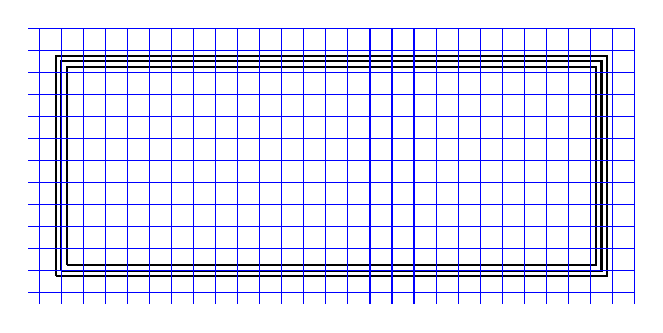
\begin{tikzpicture}[scale=0.7]
        \draw[thick] (0,0) -- (10,0) -- (10,4) -- (0,4) -- (0,0);
        \draw[thick] (0.1,0.1) -- (9.9,0.1) -- (9.9,3.9) -- (0.1,3.9) -- (0.1,0.1);
        \draw[thick] (0.2,0.2) -- (9.8,0.2) -- (9.8,3.8) -- (0.2,3.8) -- (0.2,0.2);
        
        \foreach \y in {-0.3, 0.1, 0.5, ..., 4.5}
          \draw[blue] (-0.5,\y) -- (10.5,\y);
        \foreach \x in {-0.3, 0.1, 0.5, ..., 10.5}
          \draw[blue] (\x,-0.5) -- (\x,4.5);

        %\draw[->] (0,5) -- (1,5) node[right]{x};
        %\draw[->] (0,5) -- (0,6) node[right]{y};
      \end{tikzpicture}
      } &
      \subfloat[Linear Mesh]{
        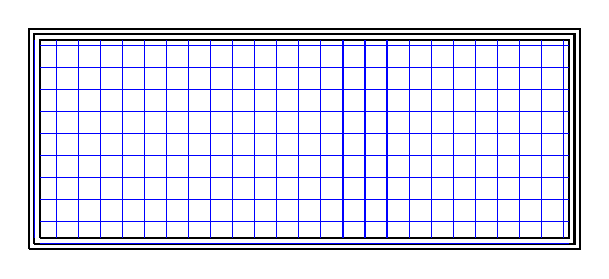
\begin{tikzpicture}[scale=0.7]
        \draw[thick] (0,0) -- (10,0) -- (10,4) -- (0,4) -- (0,0);
        \draw[thick] (0.1,0.1) -- (9.9,0.1) -- (9.9,3.9) -- (0.1,3.9) -- (0.1,0.1);
        \draw[thick] (0.2,0.2) -- (9.8,0.2) -- (9.8,3.8) -- (0.2,3.8) -- (0.2,0.2);
        \foreach \y in {0.1, 0.5, ..., 4}
          \draw[blue] (0.2,\y) -- (9.8,\y);
        \foreach \x in {0.1, 0.5, ..., 10}
          \draw[blue] (\x,0.2) -- (\x,3.8);
      \end{tikzpicture}
      }
    \end{tabular}
    \vspace{1em}
    \caption{Creating shells from the perimeter polygon}\label{fig-shells}
\end{figure*}


With\marginnote[1em]{Printer Travel Path} all the deposition lines defined for the slice, Step 4 creates the path the printer will take to deposit the filament. The printer starts with the outer perimeter path and followed by the inner parameter paths. The process then takes the linear infill lines and increments back and forth for both the horizontal and vertical lines of the mesh so that the travel of the printer head between depositions is minimised.

\begin{figure}[h!]
  \centering
    \begin{tikzpicture}[scale=1, decoration={markings,mark=at position 0.5 with {\arrow{>}}}]
      \draw[thick,postaction={decorate},->] (0,0) -- (10,0); 
      \draw[thick,postaction={decorate},->] (10,0) -- (10,4); 
      \draw[thick,postaction={decorate},->] (10,4) -- (0,4); 
      \draw[thick,postaction={decorate},->] (0,4) -- (0,0); 

      \draw[thick,postaction={decorate},->] (0.1,0.1) -- (9.9,0.1); 
      \draw[thick,postaction={decorate},->] (9.9,0.1) -- (9.9,3.9); 
      \draw[thick,postaction={decorate},->] (9.9,3.9) -- (0.1,3.9); 
      \draw[thick,postaction={decorate},->] (0.1,3.9) -- (0.1,0.1);

      \draw[thick,postaction={decorate},->] (0.2,0.2) -- (9.8,0.2); 
      \draw[thick,postaction={decorate},->] (9.8,0.2) -- (9.8,3.8); 
      \draw[thick,postaction={decorate},->] (9.8,3.8) -- (0.2,3.8); 
      \draw[thick,postaction={decorate},->] (0.2,3.8) -- (0.2,0.2);

      \foreach \y in {1.0, 2.0, 3.0, 4}
        \draw[thick,blue,postaction={decorate},->] (9.8,\y) --(0.2,\y);

      \foreach \y in {0.5, 1.5, 2.5, 3.5}
        \draw[thick,blue,postaction={decorate},->] (0.2,\y) -- (9.8,\y);
        
      \foreach \x in {0.5, 1.5, 2.5, 3.5, 4.5, 5.5, 6.5, 7.5, 8.5, 9.5}
        \draw[thick,blue,postaction={decorate},->]  (\x,3.8) -- (\x,0.2);

      \foreach \x in {1, 2, 3, 4, 5, 6, 7, 8, 9, 10}
        \draw[thick,blue,postaction={decorate},->] (\x,0.2) -- (\x,3.8);

      \draw[thick,red,->] (0,0) -- (0.1,0.1);
      \draw[thick,red,->] (0.1,0.1) -- (0.2,0.2);

      \draw[thick,red,->] (0.2,0.2) -- (0.2,0.5); 
      \draw[thick,red,->] (0.2,1.0) -- (0.2,1.5);
      \draw[thick,red,->] (0.2,2.0) -- (0.2,2.5);
      \draw[thick,red,->] (0.2,3.0) -- (0.2,3.5);

      \draw[thick,red,->] (9.8,0.5) -- (9.8,1.0); 
      \draw[thick,red,->] (9.8,1.5) -- (9.8,2.0);
      \draw[thick,red,->] (9.8,2.5) -- (9.8,3.0);

      \draw[thick,red,->] (9.8,3.5) -- (9.5,3.8); % top right diagonal

      \draw[very thick,black] (0,4.4) -- (0.2,4.4) node[pos=1.0,anchor=west] {Shell Line};
      \draw[very thick,blue] (3,4.4) -- (3.2,4.4) node[pos=1.0,anchor=west,black] {Infill Line};
      \draw[very thick,red] (6,4.4) -- (6.2,4.4) node[pos=1.0,anchor=west,black] {Travel Line};

      % [To Finish]
    \end{tikzpicture}
    \caption{Generated printer path}\label{fig-printer-path}
\end{figure}

Stage 5\marginnote{G-Code} then generates the GCode file containing the printer head movements. Before the commands are placed in the GCode, there is a pre-amble section that provides the initial settings and parameters for the printer. The co-ordinates are then translated into GCode commands that contain both the co-ordinates and feed rates for the printer filament. A post-amble is then appended to the document, which tells the printer to return to its initial state and cool down.


\subsubsection{Strengths}

One\marginnote{Convenience} of the main strengths of 3D printing is its convenience. The parts are typically a fraction of the cost compared to other prototyping methods and the process if very quick. Parts are often printed in hours enabling you to view and amend models quickly, making the design process more fluid. The process is also very simple and easy to use requiring little knowledge to get up and running. 

3D\marginnote{Structure} Printing is also incredibly flexible in the geometry that it can print and is good for small, unusual and awkwardly shaped components. It is also very good for free-form surfaces and is often used in producing casings for products. It also has a limited capability to produce some functional items including screw threads, dowels and holes, spacers and the material can also be tapped.

\subsubsection{Weaknesses}

However\marginnote{Quality and Finish}, 3D Printing is not the answer to all of your prototyping and manufacturing needs. 3D Printers still find it a challenge with features that require high tolerances. In particular, cylindricity, parallel and perpendicularity is often challenging due to the nature of printing in layers and the level of accuracy the printers can attain with the stepper motors. 

Surface quality is generally good for prototypes but post-processing is required for a truly smooth surface. Small bumps and deviations can appear on the surface as the filament cools. In addition, there is a lack of consistency in the print quality and accuracy for the same print instructions.


\subsubsection{Guidelines}

Always\marginnote{Evaluate Different Orientations} double check whether the model has been placed in its optimum position for printing. Re-orienting the model within the slicing software can significantly reduce number of supports that may be required.

Even-though\marginnote{Avoid Overhangs} 3D printing can deal with overhangs by using supports, significant reductions in manufacturing time can be achieved by generating geometry that does not require the use of supports. This reduces manufacturing time as supports do not need to be printed, a reduction in material use and post-processing time owing to the need to remove them from the structure.

The\marginnote{Keep to Low Infill Densities} process is also less suitable for large parts and parts, which require 100\% infill. This is due to the time it takes and the greater likelihood of the print failing due to printer operating for a long time.

Although\marginnote{Place Prints near the Centre of the Bed} the printers are regularly calibrated, it is still good practice to place the component near the centre of the bed. And even-though the printers can handle the printing of multiple parts at once, this introduces issues in the filament maintaining adhesion between layers as the component will cool whilst the printer head is busy on a different component.

\section{Project Management Essentials}

Managing engineering projects is not an easy task. There is potential for requirement scope creep and given the lead-times in a products design, there is a lot of staff churn and unforeseen issues that might arise. In this section, we will be introducing you to a set of essential project management tools and methods that are used in industry. These are:

\begin{itemize}
    \item Action Tracking;
    \item \acf{BOM};
    \item \acf{PERT};
    \item Risk Mitigation; and,
    \item Cost/Resource Modelling
\end{itemize}


\subsection{Action Tracking}

Action tracking is the activity of assigning and monitoring of actions amongst team members within a project. Typically performed at meetings, actions are recorded and then assigned an owner whose responsible for getting the action completed. This does not necessarily mean doing the action themselves and subsequent delegation and/or teamwork may be required to support the owner in completing the action. Many companies employ action tracking to ensure project progression and maintaining balanced workloads amongst their employees.

Action trackers can come in many forms but a typical set-up is to use a spreadsheet as shown in \cref{tab:action-tracker}.

\begin{table*}[h]
    \centering
    \resizebox{\textwidth}{!}{
    \begin{tabular}{r l l r r r r r}
        \toprule
            \# & Action & Owner & Date Created & Date Completed & Hours Allocated & Hours Accrued & Status \\
        \midrule
            1 & An example action & EG & 01/01/1980 & 10/01/1980 & 2.00 & 3.00 & Completed \\
            2 & Another example & EG & 03/01/1980 & 20/01/1980 & 3.00 & 3.00 & Incomplete \\
        \bottomrule
    \end{tabular}
    }
    \caption{Example Action Tracker}
    \label{tab:action-tracker}
\end{table*}

\subsection{Bill of Materials}

A \acf{BOM} is a list of the raw materials, sub-assemblies, intermediate assemblies, sub-components, parts and the quantities of each needed to manufacture an end product. This often comes in the form of a spreadsheet but it is more and more common to have the \ac{BOM} generated by the \acf{CAD}/\acf{PLM} systems used by the company. The key benefit is that that \ac{BOM} will automatically update to include any design changes that are made by the engineers.


\subsection{Project Evaluation and Review Techniques (PERT)} 

\acf{PERT} are methods of analysing the tasks involved in completing a given project, especially the time needed to complete each task, to identify the minimum time needed to complete the project\cite{vanhoucke2012}. 
It can be considered to be a sub-section of graph theory where the aim is to identify the critical paths between tasks.

It incorporates uncertainty by making it possible to schedule a project while not knowing precisely the details and durations of all the activities. It is more of an event-oriented technique rather than start/completion -oriented, and is used more in projects where time is the major factor rather than cost. It has been applied to many large-scale, one-time, complex, non-routine infrastructure and Research \& Development projects.

\ac{PERT} involves the generation of a graph where the vertices refer to tasks and the edges represent dependencies between the tasks. In contrast to \acf{CPM}, where the edges would be weighted by a single metric, \ac{PERT} applies three metrics for the time it will take for an activity to complete. \ac{PERT} defines four types of time relating to an activity.

\begin{table}
  \small
  \begin{tabular}{r p{0.7\textwidth}}
    Optimistic & The minimum possible time required to accomplish an activity ($o$) or a path ($O$), assuming everything proceeds better than is normally expected. \\
    Pessimistic & The maximum possible time required to accomplish an activity ($p$) or a path ($P$), assuming everything goes wrong (but excluding major catastrophes). \\
    Most Likely Time & The best estimate of the time required to accomplish an activity ($m$) or a path ($M$), assuming everything proceeds as normal. \\
    Expected Time & The best estimate of the time required to accomplish an activity ($e$) or a path ($E$), which is derived from the previous time estimates using \cref{equ-time}.
  \end{tabular}
\end{table}

\begin{equation}
  e = \frac{o+4m+p}{6}
  \label{equ-time}
\end{equation}

One can also calculate the standard deviation for the expected time based on $o$ and $p$.

\begin{equation}
  \sigma_e = \frac{p-o}{6}
\end{equation}

With these metrics and the activity graph, we are then able to determine:

\begin{table}
  \small
  \begin{tabular}{r p{0.7\textwidth}}
    Float (Slack) & This a measure of the excess time and resources available to complete a task. It is the amount of time that a project task can be delayed without causing a delay in any subsequent tasks (free float) or the whole project (total float). Positive float would indicate ahead of schedule; negative float would indicate behind schedule; and zero float would indicate on schedule. \\
    Critical Path & The longest possible continuous pathway taken from the initial event to the terminal event. It determines the total calendar time required for the project; and, therefore, any time delays along the critical path will delay the reaching of the terminal event by at least the same amount. \\
    Critical Activity & An activity that has total float equal to zero. An activity with zero float is not necessarily on the critical path since its path may not be the longest. \\
    Lead time & The time by which a predecessor event must be completed in order to allow sufficient time for the activities that must elapse before a specific \ac{PERT} event reaches completion. \\
    Lag time & The earliest time by which a successor event can follow a specific \ac{PERT} event. \\
    Fast Tracking & Performing critical activities in parallel. \\
    Crashing Critical Path & Shortening duration of critical activities. \\
  \end{tabular}
\end{table}


\cref{tbl-project}\marginnote{Example} contains seven tasks that represent the work that needs to be performed for a project. Some tasks have dependencies on others whilst some tasks can be performed concurrently. The time estimates for the tasks have been provided for each of the tasks. In your case, these tasks would represent the manufacture, handling and assembly times for your Design \& Make.

\begin{table}[h!]
  \centering
  \begin{tabular}{l l r r r r}
  \toprule
    Activity & Predecessor & \multicolumn{4}{c}{Time Estimates} \\
    & & $o$ & $m$ & $p$ & $e$ \\
  \midrule
    A & -- & 2 & 4 & 6 & 4.00 \\
    B & -- & 3 & 5 & 9 & 5.33 \\
    C & A & 4 & 5 & 7 & 5.17 \\
    D & A & 4 & 6 & 10 & 6.33 \\
    E & B, C & 4 & 5 & 7 & 5.17 \\
    F & D & 3 & 4 & 8 & 4.50 \\
    G & E & 3 & 5 & 8 & 5.17 \\
  \bottomrule
  \end{tabular}
  \caption{Example project}\label{tbl-project}
\end{table}

From this information, we can generate a graph showing how the tasks are connected with one another (Figure~\ref{fig-pert-graph}). Each vertex in the graph contains:

\begin{itemize}
  \item Task name
  \item Expected Time ($e$)
  \item Early start time (ES)
  \item Early finish time (EF)
  \item Late start time (LS)
  \item Late finish time (LF)
  \item Float
\end{itemize}

To calculate these values, the process is as follows:

\begin{description}
  \item[Step 1] Calculate the Early Start ($ES$) and Early Finish ($EF$) times for each vertex.
  \item[Step 2] Calculate the Late Start ($LS$) and Late Finish ($LF$) times for each vertex.
  \item[Step 3] Calculate the float for each vertex and identify the critical path.
\end{description}

The results are this process is shown in Figure~\ref{fig-pert-graph}

Step 1\marginnote{Step One} is to calculate the Early Start ($ES$) and Early Finish ($EF$) times for each vertex. $ES$ is defined as the maximum $EF$ of all predecessor activities, unless the activity in question is the first activity, for which $ES=0$. EF is ES plus the expected task duration ($e$).

\begin{equation}
  EF = ES + e
\end{equation}

If\marginnote{Step Two} everything runs smoothly, the project should take 19.51 work days to complete. With this information, we can work backwards to determine the Late Start ($LS$) and Late Finish ($LF$) times for each task. $LF$ is defined as the minimum $LS$ of all successor activities, unless the activity is the last activity, for which the $LF=EF$. The $LS$ is the $LF$ minus the task duration.

\begin{figure*}[t!]
    \centering
    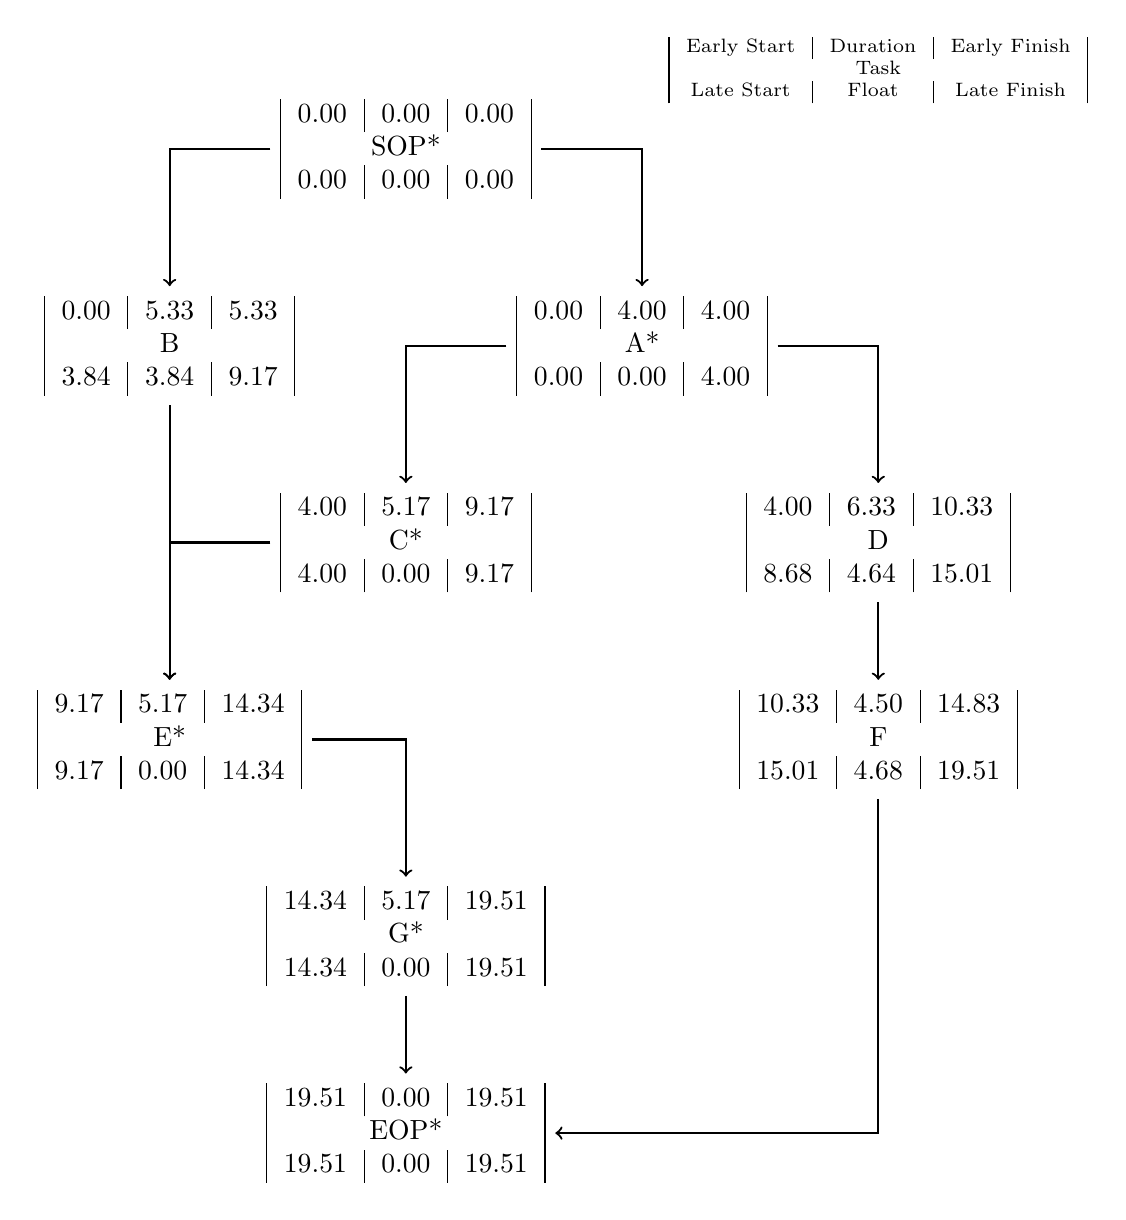
\begin{tikzpicture}

    \node[] (SOP) at (0,0) {
      \begin{tabular}{|c|c|c|}
        \midrule
          0.00 & 0.00 & 0.00 \\
        \midrule
          \multicolumn{3}{|c|}{SOP*} \\
        \midrule
          0.00 & 0.00 & 0.00 \\
        \midrule
      \end{tabular}
    };

    \node[] (A) at (3,-2.5) {
      \begin{tabular}{|c|c|c|}
        \midrule
          0.00 & 4.00 & 4.00 \\
        \midrule
          \multicolumn{3}{|c|}{A*} \\
        \midrule
          0.00 & 0.00 & 4.00 \\
        \midrule
      \end{tabular}
    };

    \node[] (B) at (-3,-2.5) {
      \begin{tabular}{|c|c|c|}
        \midrule
          0.00 & 5.33 & 5.33 \\
        \midrule
          \multicolumn{3}{|c|}{B} \\
        \midrule
          3.84 & 3.84 & 9.17 \\
        \midrule
      \end{tabular}
    };

    \node[] (D) at (6,-5) {
      \begin{tabular}{|c|c|c|}
        \midrule
          4.00 & 6.33 & 10.33 \\
        \midrule
          \multicolumn{3}{|c|}{D} \\
        \midrule
          8.68 & 4.64 & 15.01 \\
        \midrule
      \end{tabular}
    };

    \node[] (C) at (0,-5) {
      \begin{tabular}{|c|c|c|}
        \midrule
          4.00 & 5.17 & 9.17 \\
        \midrule
          \multicolumn{3}{|c|}{C*} \\
        \midrule
          4.00 & 0.00 & 9.17 \\
        \midrule
      \end{tabular}
    };

    \node[] (F) at (6,-7.5) {
      \begin{tabular}{|c|c|c|}
        \midrule
          10.33 & 4.50 & 14.83 \\
        \midrule
          \multicolumn{3}{|c|}{F} \\
        \midrule
          15.01 & 4.68 & 19.51 \\
        \midrule
      \end{tabular}
    };

    \node[] (E) at (-3,-7.5) {
      \begin{tabular}{|c|c|c|}
        \midrule
          9.17 & 5.17 & 14.34 \\
        \midrule
          \multicolumn{3}{|c|}{E*} \\
        \midrule
          9.17 & 0.00 & 14.34 \\
        \midrule
      \end{tabular}
    };

    \node[] (G) at (0,-10) {
      \begin{tabular}{|c|c|c|}
        \midrule
          14.34 & 5.17 & 19.51 \\
        \midrule
          \multicolumn{3}{|c|}{G*} \\
        \midrule
          14.34 & 0.00 & 19.51 \\
        \midrule
      \end{tabular}
    };

    \node[] (EOP) at (0,-12.5) {
      \begin{tabular}{|c|c|c|}
        \midrule
          19.51 & 0.00 & 19.51 \\
        \midrule
          \multicolumn{3}{|c|}{EOP*} \\
        \midrule
          19.51 & 0.00 & 19.51 \\
        \midrule
      \end{tabular}
    };

    \node[] (Index) at (6,1) {
      \scriptsize
      \begin{tabular}{|c|c|c|}
        \midrule
          Early Start & Duration & Early Finish \\
        \midrule
          \multicolumn{3}{|c|}{Task} \\
        \midrule
          Late Start & Float & Late Finish \\
        \midrule
      \end{tabular}
    };

    \draw[thick, ->] (SOP) -| (A);
    \draw[thick, ->] (SOP) -| (B);
    \draw[thick, ->] (A) -| (C);
    \draw[thick, ->] (A) -| (D);
    \draw[thick, ->] (B) -- (E);
    \draw[thick, ->] (C) -| (E);
    \draw[thick, ->] (D) -- (F);
    \draw[thick, ->] (E) -| (G);
    \draw[thick, ->] (F) |- (EOP);
    \draw[thick, ->] (G) -- (EOP);

    \end{tikzpicture}
    \vspace{1em}
    \caption{Project task graph}\label{fig-pert-graph}
\end{figure*}


\begin{equation}
  LS = LF - e
\end{equation}

Having\marginnote{Step Three} calculated $LS$ and $LF$ for each task, we can calculate the float for each activity. Float is equal to $LF - EF$ or $LS - ES$ as these are equivalent. This enables us to identify the critical path activities, which are indicated by the task having zero float.

%\marginlabel{Gantt Chart}

This\marginnote{Further Analysis} is as far as we will go with \ac{PERT} analysis for the Design \& Make exercise however, there is much more analysis that can be performed using this graph to provide organisations more information on the potential risk within the project. One example is the ability to automate the generation of these values so that you can perform a Monte-Carlo simulation based on the time distributions (known as \ac{PERT}-beta distributions). This analysis can provide insights in the potential variance in the critical path and the likelihood of the path changing depending on the task times\cite{davis2008}.

More advanced \ac{PERT} analysis also enables the inclusion of resource constraints, which limit the number of concurrent tasks. This could be due to a limitation in the availability of labour, machines and/or costed time.

A Python Notebook of the \ac{PERT} analysis procedure is available at: \\ \url{https://tinyurl.com/y72kjxfo}


\subsection{Risk Mitigation} 

All engineering projects carry risks and it is important to capture and monitor the potential risks as a project progresses. It is the duty of engineers to communicate risks clearly and effectively, and to propose solutions that will aid in mitigating risks to a project. In fact, we have already started to look at risks by using PERT to analyse and map out the plan of tasks for the project.

One\marginnote{Risk Register} method of capturing and monitoring risks within an engineering project is through the development of a risk register (\cref{tbl-risk}).

\begin{table}[h!]
  \centering
  \caption{Example Risk Register}
  \label{tbl-risk}
  \begin{tabular}{l l l l l l}
    \toprule
      No. & Risk & Impact & Chance & Owner & Mitigation \\
    \midrule
      1 \\
      2 \\
      3 \\
      \ldots \\
    \bottomrule
  \end{tabular}
\end{table}

An\marginnote{Example Risk} example in the Design \& Make project would be that a manufacturing machine (e.g\ Laser Cutter) for the manufacture of a gear is offline and requires maintenance. The impact of this is that a component will not be manufactured in time. The chance of this occurring is often attained through analysis of historical project data and analysis of the reliability of the machine. The owner may be the project manager but ideally risks should be equally shared amongst the team. So in this case, it may be best to give this risk to the engineer who designed and analysed the manufacturability of the product. We then have to come up with a strategy to mitigate the impact of this risk to the project. For this example, suggestions could be to have a alternative manufacturing strategy such as 3D printing or to purchase a gear from a supplier at an additional cost to the project.

Risks cover as many potential issues that the project could encounter. You should also be including issues where one of the team may be absent during the week that you intend to manufacture \& assemble the product.

This register will be very important during 2nd semester and during the presentation of your prototype, we would like you to reflect on the production of the product and whether you encountered any of these risks as well as any other issues that may have not been identified.

\subsection{Cost/Resource Modelling}

There are numerous sources that impact the cost and level of resource required for a project. In this exercise, we want to broaden your understanding of what cost means to a project and where it might come from.

During\marginnote{suppliers} your design work, you have been looking at supplier catalogues for potential sources of components. In this exercise, you will be solely focusing on the price of the components they offer but in a large organisation there are additional costs incurred such as contracts, stakeholder engagement, logistics and the resolving of issues if components are not to specification. 

For\marginnote{raw materials} each component you will be manufacturing in-house, there is a cost associated with the raw materials that you will be purchasing. As with the stock market, raw materials prices can change on a regular basis based on supply and demand at the time. Thus, large organisations often have to hedge and buy material in advance to have security that the material will be available to them but this also comes at an additional cost.

This\marginnote{machining} is the cost of manufacturing the components that you have designed. In this project, you have looked at the time to machine a single prototype component but in production projects there are additional costs such as those relating to the maintenance of the machines, cost of tooling (drill bits, dies, coolant) and energy/facility use.

In\marginnote{assembly} addition to machining, there is the cost of assembly, which you have been analysing during the design of your product. Again, there would be additional costs in the facilities required for this assembly line to function and the need to store components before and after assembly.

Then\marginnote{human resources} there is the human resource involved in the project and this is covers all the time spent designing, manufacturing and the cost of the personnel that need to be involved, which features pay scales, national insurance contributions, holiday entitlements and pensions to name a few. All these are factored into an engineers' hourly rate when being costed to projects.

In\marginnote{currency exchange rates} large organisations, the currency exchange rates can play a huge factor in to revenue and cost modelling of projects. This is where companies have order books looking ahead 20 years and predictions have to be made on the price the quote and the future cost. One example of the consequence of exchanges rates is Rolls-Royce having to write-down \textsterling2bn after the brexit vote due to the dip in the pound.\cite{tovey2016}

The list could continue and include:

\begin{itemize}
  \item Waste handling
  \item End-of-life recycling
  \item Logistics
  \item Offices
  \item Administrative services
  \item Maintenance \& service agreements
\end{itemize}


\RaggedRight
\bibliography{citations}
\bibliographystyle{plainnat}

\end{document}